\documentclass[a4paper, 12pt]{article}
\usepackage[francais]{babel}
\usepackage{fontspec}
\usepackage{enumitem}
\usepackage{authblk}
\usepackage{pdfpages}
\usepackage{minted}
\definecolor{bg}{RGB}{246,248,250}
\newminted{rust}{fontsize=\footnotesize,tabsize=4,frame=single,linenos}
\newminted{shell}{tabsize=4}
\usepackage{dirtree}
\usepackage{amsmath}
\usepackage{hyperref}
\usepackage{tabularx}
\usepackage{multirow}
\usepackage{multicol}
\usepackage{wrapfig}
\newcolumntype{C}[1]{>{\centering\arraybackslash}p{#1}}
\setlength{\parindent}{0pt}
\usepackage{hyperref}
\hypersetup{
    colorlinks,
    citecolor=black,
    filecolor=black,
    linkcolor=black,
    urlcolor=blue
}
\usepackage{caption}
\newenvironment{code}{\captionsetup{type=listing,skip=-10pt}}{}
\usepackage{etoolbox}
\patchcmd{\thebibliography}{\section*{\refname}}{}{}{}
\usepackage[left=2.5cm,top=2.5cm,right=2.5cm,bottom=2.5cm]{geometry}
\usepackage{glossaries}
	\let\oldnewacronym\newacronym
	\newcommand*{\provideacronym}[3]{%
	  \ifglsentryexists{#1}{%
	  }{%
	    \oldnewacronym{#1}{#2}{#3}%
	  }%
	}
\makeglossaries

%%%%%%%%%%%%%%%%%%%%%%%%%%%%%%%%%%%%%%%%%%%%%%%%%%%%%%%%%%%%%%%%%%
%%%%%%%%%%%%%%%%%%%%%%%%%%%%%%%%%%%%%%%%%%%%%%%%%%%%%%%%%%%%%%%%%%

\begin{document}
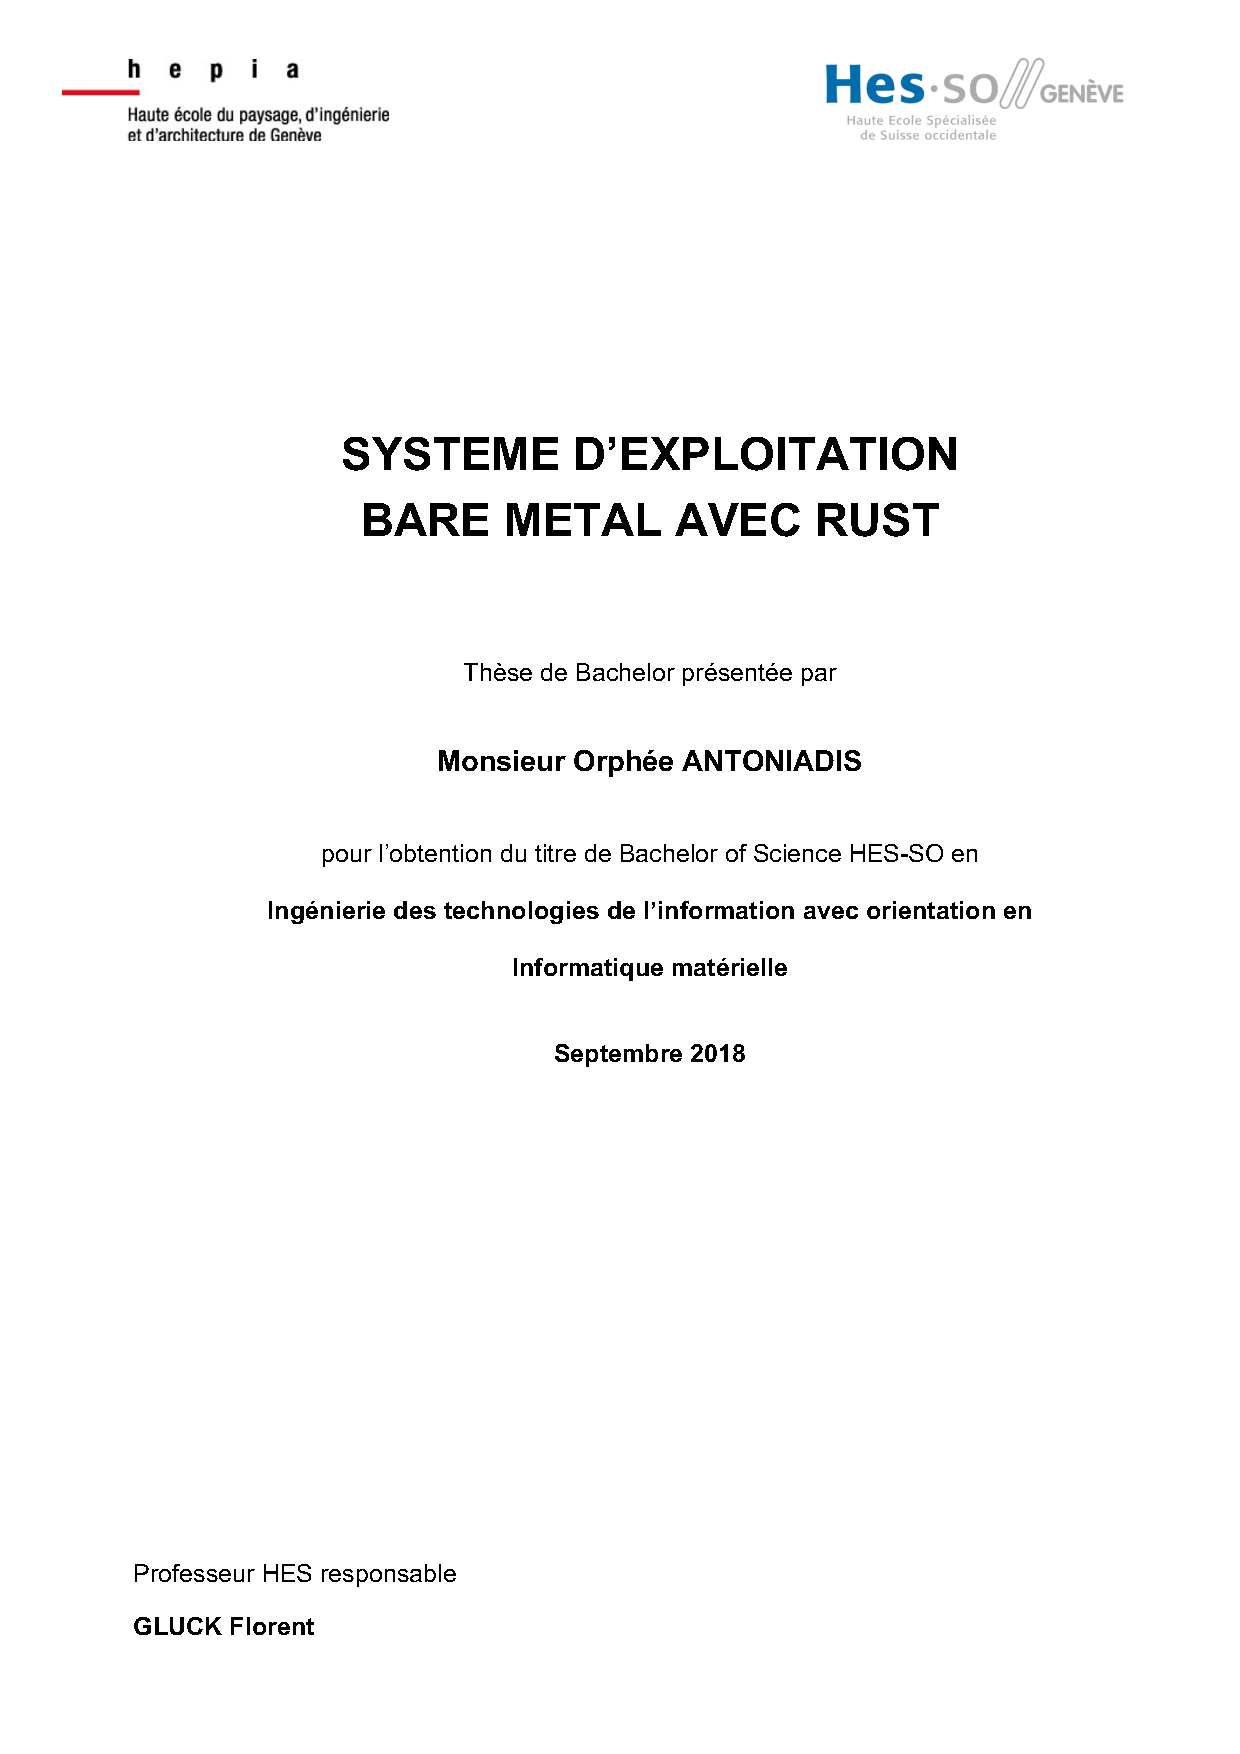
\includepdf[pages=1]{../ITI_masque_couverture.pdf}

\newpage
\thispagestyle{empty}
\clearpage\mbox{}\clearpage
\pagenumbering{arabic}

%%%%%%%%%%%%%%%%%%%%%%%%%%%%%%%%%%%%%%%%%%%%%%%%%%%%%%%%%%%%%%%%%%
%%%%%%%%%%%%%%%%%%%%%%%%%%%%%%%%%%%%%%%%%%%%%%%%%%%%%%%%%%%%%%%%%%

\addcontentsline{toc}{section}{Descriptif}
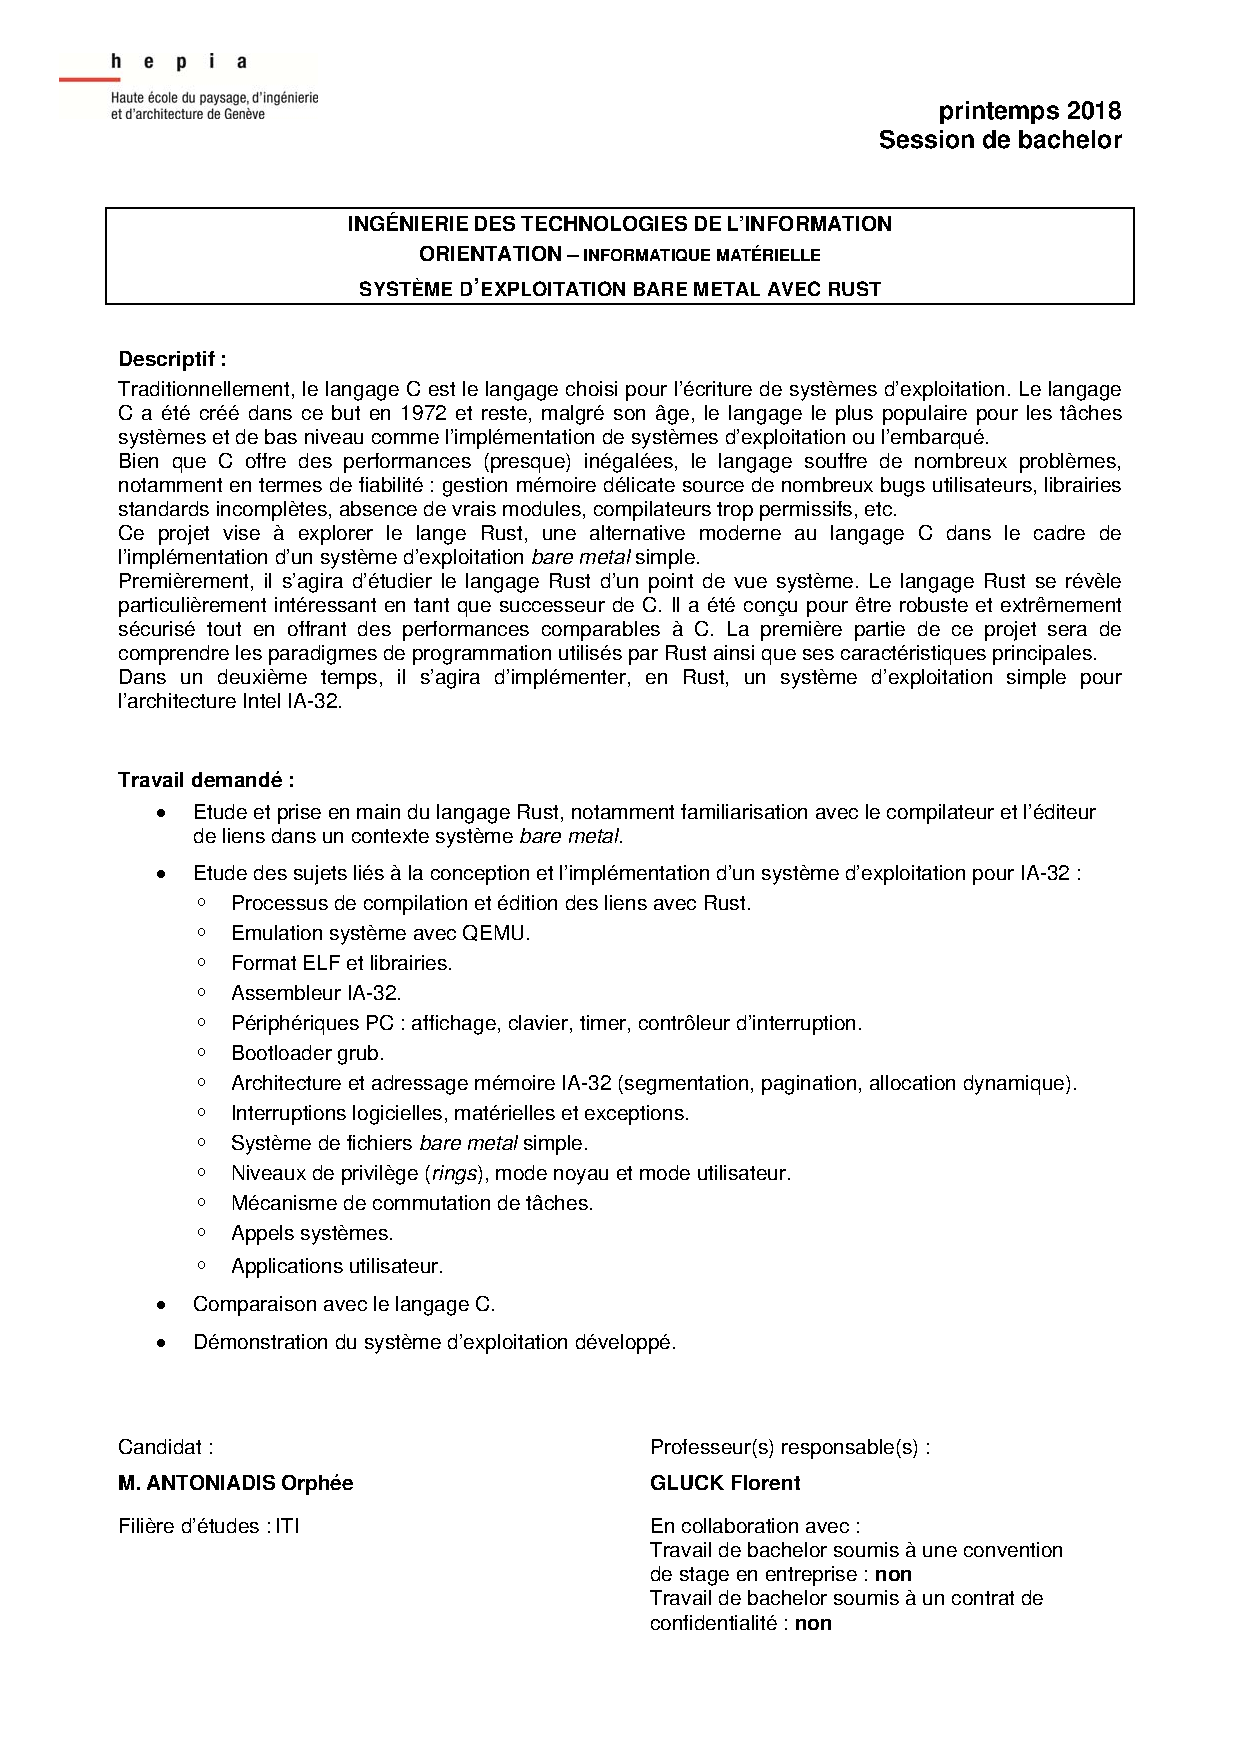
\includepdf[pages=1]{../ITI_MAT_jour_enonce_diplome_Antoniadis_Gluck_2018.pdf}

\newpage
\thispagestyle{empty}
\clearpage\mbox{}\clearpage

%%%%%%%%%%%%%%%%%%%%%%%%%%%%%%%%%%%%%%%%%%%%%%%%%%%%%%%%%%%%%%%%%%
%%%%%%%%%%%%%%%%%%%%%%%%%%%%%%%%%%%%%%%%%%%%%%%%%%%%%%%%%%%%%%%%%%

\addcontentsline{toc}{section}{Résumé}
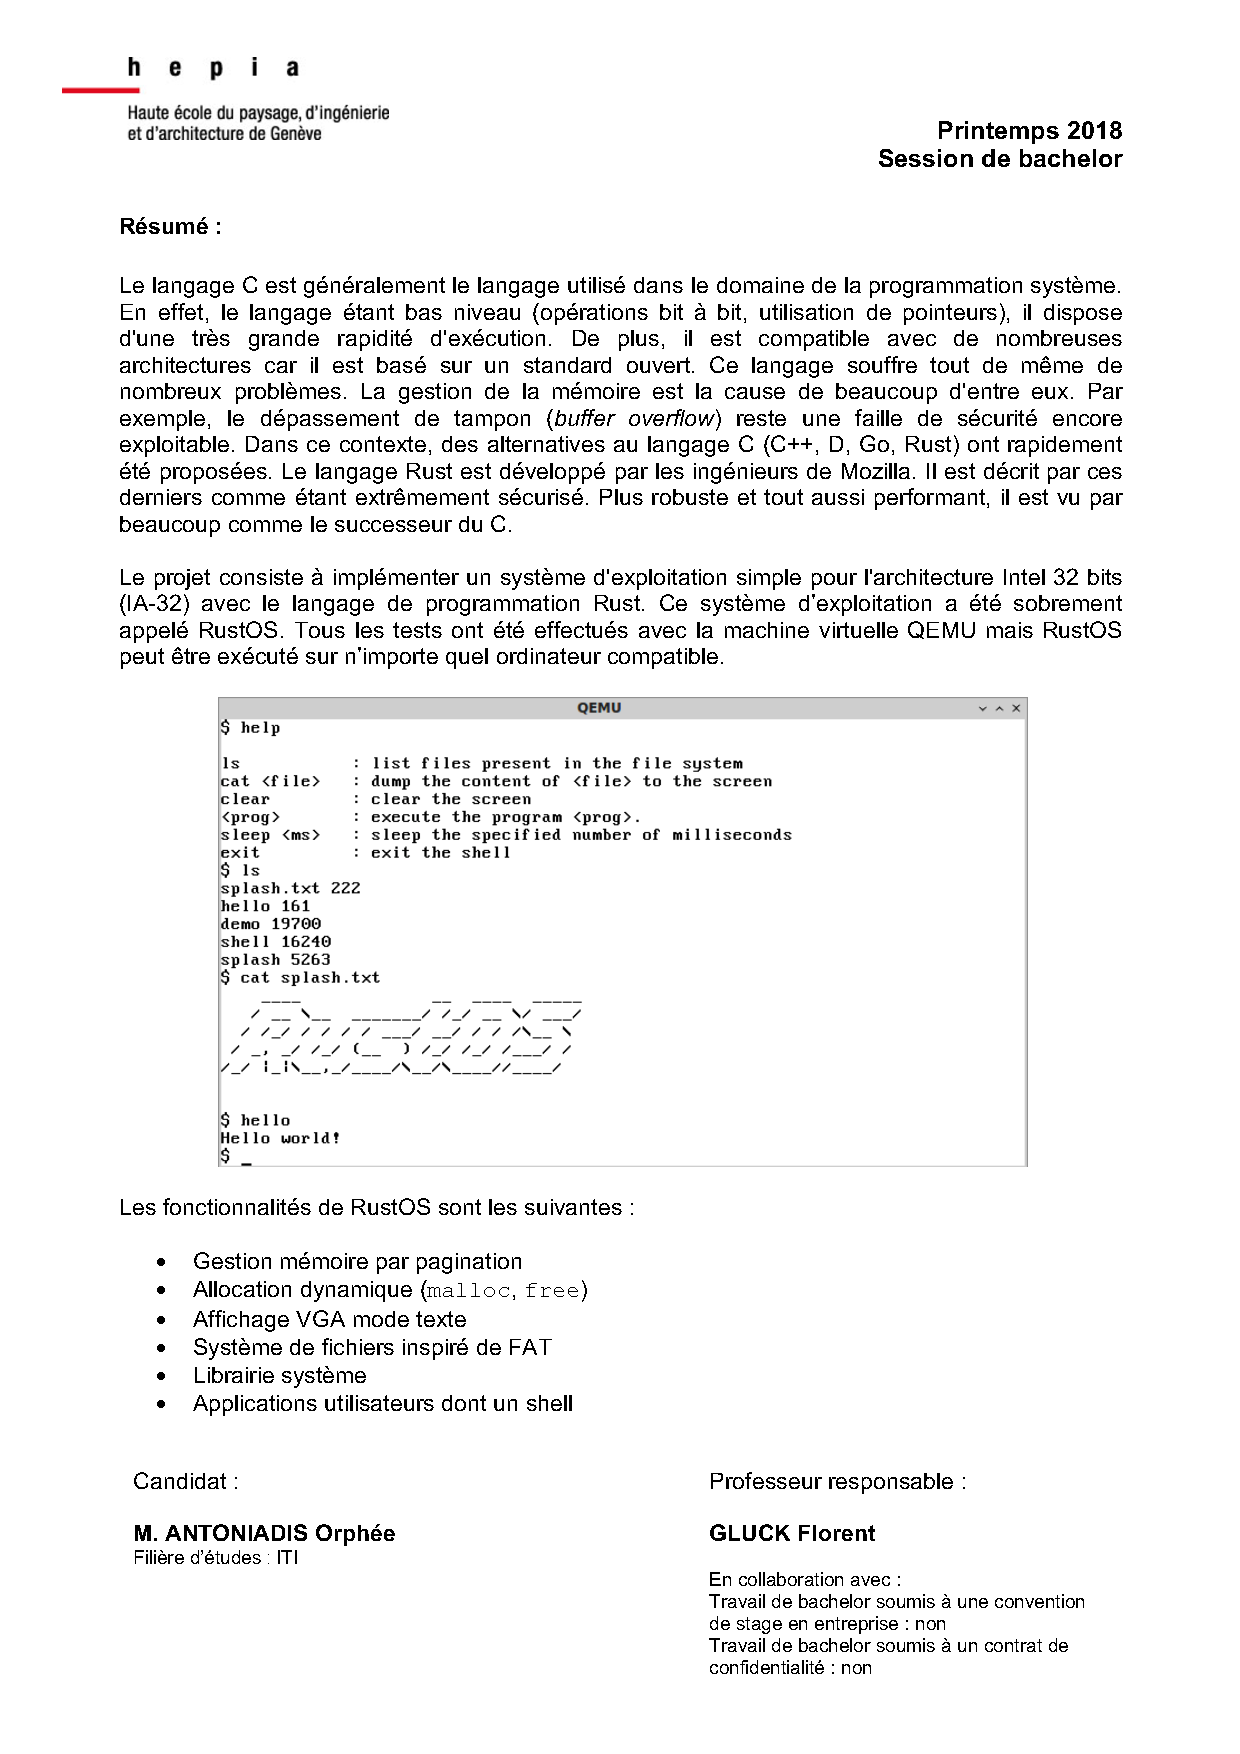
\includepdf[pages=1]{../ITI_masque_resume_diplome_2018.pdf}

\newpage
\thispagestyle{empty}
\clearpage\mbox{}\clearpage

%%%%%%%%%%%%%%%%%%%%%%%%%%%%%%%%%%%%%%%%%%%%%%%%%%%%%%%%%%%%%%%%%%
%%%%%%%%%%%%%%%%%%%%%%%%%%%%%%%%%%%%%%%%%%%%%%%%%%%%%%%%%%%%%%%%%%

\newpage
\setcounter{tocdepth}{2}
\addcontentsline{toc}{section}{Table des matières}
\tableofcontents

%%%%%%%%%%%%%%%%%%%%%%%%%%%%%%%%%%%%%%%%%%%%%%%%%%%%%%%%%%%%%%%%%%
%%%%%%%%%%%%%%%%%%%%%%%%%%%%%%%%%%%%%%%%%%%%%%%%%%%%%%%%%%%%%%%%%%

\newpage
\addcontentsline{toc}{section}{Table des figures}
\listoffigures

%%%%%%%%%%%%%%%%%%%%%%%%%%%%%%%%%%%%%%%%%%%%%%%%%%%%%%%%%%%%%%%%%%
%%%%%%%%%%%%%%%%%%%%%%%%%%%%%%%%%%%%%%%%%%%%%%%%%%%%%%%%%%%%%%%%%%

\newpage
\addcontentsline{toc}{section}{Table des tables}
\renewcommand{\listtablename}{Table des tables}
\listoftables

%%%%%%%%%%%%%%%%%%%%%%%%%%%%%%%%%%%%%%%%%%%%%%%%%%%%%%%%%%%%%%%%%%
%%%%%%%%%%%%%%%%%%%%%%%%%%%%%%%%%%%%%%%%%%%%%%%%%%%%%%%%%%%%%%%%%%

\newpage
\addcontentsline{toc}{section}{Table des \textit{listings} de code}
\renewcommand\listoflistingscaption{Table des \textit{listings} de code}
\listoflistings

%%%%%%%%%%%%%%%%%%%%%%%%%%%%%%%%%%%%%%%%%%%%%%%%%%%%%%%%%%%%%%%%%%
%%%%%%%%%%%%%%%%%%%%%%%%%%%%%%%%%%%%%%%%%%%%%%%%%%%%%%%%%%%%%%%%%%

\newpage
\addcontentsline{toc}{section}{Acronymes}
\newacronym{os}{OS}{\textit{Operating System}}
\newacronym{elf}{ELF}{\textit{Executable and Linkable Format}}
\newacronym{gcc}{GCC}{\textit{GNU Compiler Collection}}
\newacronym{iso}{ISO}{\textit{International Organization for Standardization}}
\newacronym{vram}{VRAM}{\textit{Video Random Access Memory}}
\newacronym{grub}{GRUB}{\textit{GRand Unified Bootloader}}
\newacronym{bios}{BIOS}{\textit{Basic Input Output System}}
\newacronym{pc}{PC}{\textit{Personal Computer}}
\newacronym{mbr}{MBR}{\textit{Master Boot Record}}
\newacronym{gdt}{GDT}{\textit{Global Descriptor Table}}
\newacronym{idt}{IDT}{\textit{Interrupt Descriptor Table}}
\newacronym{vga}{VGA}{\textit{Video Graphics Array}}
\newacronym{pio}{PIO}{\textit{Port Input/Output}}
\newacronym{cpu}{CPU}{\textit{Central Processing Unit}}
\newacronym{IA-32}{IA-32}{\textit{Intel Architecture 32 bits}}
\newacronym{ram}{RAM}{\textit{Random Access Memory}}
\newacronym{mmu}{MMU}{\textit{Memory Management Unit}}
\newacronym{ldt}{LDT}{\textit{Local Descriptor Table}}
\newacronym{mmio}{MMIO}{\textit{Memory Mapped Input/Output}}
\newacronym{nmi}{NMI}{\textit{Non Maskable Interrupt}}
\newacronym{irq}{IRQ}{\textit{Interrupt Request}}
\newacronym{isr}{ISR}{\textit{Interrupt Service Routine}}
\newacronym{pic}{PIC}{\textit{Programmable Interrupt Controller}}
\newacronym{crtc}{CRTC}{\textit{Cathode Ray Tube Controller}}
\newacronym{pit}{PIT}{\textit{Programmable Interval Timer}}
\newacronym{tss}{TSS}{\textit{Task State Segment}}
\newacronym{fat}{FAT}{\textit{File Allocation Table}}
\newacronym{api}{API}{\textit{Application Programming Interface}}
\newacronym{posix}{POSIX}{\textit{Portable Operating System Interface}}
\newacronym{toml}{TOML}{\textit{Tom’s Obvious, Minimal Language}}
\newacronym{abi}{ABI}{\textit{Application Binary Interface}}
\newacronym{json}{JSON}{\textit{JavaScript Object Notation}}
\newacronym{nasm}{NASM}{\textit{Netwide Assembler}}
\printglossary[type=\acronymtype,title={Acronymes}]

%%%%%%%%%%%%%%%%%%%%%%%%%%%%%%%%%%%%%%%%%%%%%%%%%%%%%%%%%%%%%%%%%%
%%%%%%%%%%%%%%%%%%%%%%%%%%%%%%%%%%%%%%%%%%%%%%%%%%%%%%%%%%%%%%%%%%

\newpage
\section*{Avant-propos}
\addcontentsline{toc}{section}{Avant-propos}

\subsection*{Présentation}
Ce mémoire constitue l'aboutissement de 11 semaines de travail dans le cadre de
l'obtention du titre de Bachelor en Ingénierie des Technologies de l'Information,
orientation informatique matérielle, à hepia. Le projet consiste à implémenter
un système d'exploitation simple pour l'architecture \acrshort{IA-32} avec le langage
de programmation Rust. Ce document commence par introduire le sujet en rappelant
les objectifs et en décrivant l'architecture du système. Les caractéristiques principales
du langage Rust sont ensuite détaillées. L'implémentation du sysème d'exploitation
est expliquée en plusieurs parties. Nous nous intéressons en premier lieu à la
compilation et à l'exécution du système. Nous voyons ensuite les différentes techniques
de gestion mémoire utilisées (segmentation, pagination, allocation dynamique).
Après cela, nous nous intéressons à la manière dont un processeur Intel 32 bits
permet de communiquer avec ses périphériques (ports d'entrées/sorties, interruptions).
Le système de fichiers développé pour notre système est ensuite présenté. Enfin,
nous expliquons le fonctionnement du mode utilisateur et les différents mécanismes
permettant à une application utilisateur de communiquer avec le \textit{kernel}.
Ce rapport se termine par une présentation des résultats, une partie de discussions
au sujet des problèmes rencontrés, des améliorations possibles et des différences
entre le Rust et le C avant de conclure sur le bilan du travail accompli.

\subsection*{Conventions typographiques}
Lors de la rédaction de ce document, les conventions typographiques ci-dessous ont
été adoptées.
\begin{itemize}[label=\textbullet]
	\item Tous les mots empruntés à la langue anglaise sont écrits en \textit{italique}
	\item Toute référence à un nom de fichier (ou dossier), un chemin d’accès, une 
    utilisation de paramètre, variable, ou commande utilisable par l’utilisateur, 
    est écrite avec la police d’écriture \mintinline{rust}{Courier New}.
	\item Tout extrait de fichier ou de code est écrit selon le format suivant:
\begin{rustcode}
fn main() {
    println!("Hello, world!");
}
\end{rustcode}
    \item Toute commande importante dans le cadre du projet est écrite selon le
    format suivant:
\begin{shellcode}
$ echo Hello world!
\end{shellcode}
\end{itemize}

\subsection*{Remerciements}
J'aimerais remercier l'équipe enseignante pour la qualité de leurs enseignements,
leur implication et leur pédagogie que j'ai pu apprécier au long de ces trois
années passées à hepia. Merci à M. Glück, qui m'a suivi tout le long de ce travail
de Bachelor, pour son aide et ses conseils. Merci à ma famille et à mes proches
d'avoir été présents pendant toutes mes études. Pour finir, merci à Camille pour la
relecture de ce mémoire mais surtout pour m'avoir soutenu et supporté durant ces
11 semaines.

%%%%%%%%%%%%%%%%%%%%%%%%%%%%%%%%%%%%%%%%%%%%%%%%%%%%%%%%%%%%%%%%%%
%%%%%%%%%%%%%%%%%%%%%%%%%%%%%%%%%%%%%%%%%%%%%%%%%%%%%%%%%%%%%%%%%%

\newpage
\section{Introduction}
\subsection{Contexte}
Le langage C est généralement le langage utilisé dans le domaine de la programmation
système. En effet, le langage étant bas niveau (opérations bit à bit, utilisation
de pointeurs), il dispose d'une très grande rapidité d'exécution. De plus, il est
compatible avec de nombreuses architectures car il est basé sur un standard ouvert.
Ce langage souffre tout de même de nombreux problèmes. La gestion de la mémoire
est la cause de beaucoup d'entre eux. Par exemple, le dépassement de tampon
(\textit{buffer overflow}) reste une faille de sécurité encore exploitable.
Dans ce contexte, des alternatives au langage C (C++, D, Go, Rust) ont rapidement
été proposées. Le langage Rust est développé par les ingénieurs de Mozilla. Il
est décrit par ces derniers comme étant extrêmement sécurisé. Plus robuste et tout
aussi performant, il est vu par beaucoup comme le successeur du C.

%%%%%%%%%%%%%%%%%%%%%%%%%%%%%%%%%%%%%%%%%%%%%%%%%%%%%%%%%%%%%%%%%%

\subsection{Objectifs}
L'objectif principal de ce projet est d'implémenter un système d'exploitation
avec le langage Rust. Une première partie a donc été un travail de recherche
sur le langage. Le but était de comprendre le fonctionnement de Rust, ses caractéristiques
principales ainsi que ses spécificités. De plus, il a fallu étudier son utilisation
dans le cadre de la programmation système et plus précisémment dans le développement
d'un système d'exploitation \textit{bare metal}. La seconde partie a été l'implémentation
du système d'exploitation en question pour l'architecture \acrshort{IA-32}. Une étude
des sujets liés à la conception d'\acrshort{os} pour cette architecture a été faite.
Le deuxième objectif de ce projet est de comparer le langage Rust au langage C.
On a vu que le Rust est considéré comme étant le successeur du C. La programmation
d'\acrshort{os} est un bon contexte pour les comparer étant donnée qu'actuellement,
la majorité des systèmes d'exploitation sont en C. Pour résumer, ce travail de
Bachelor a suivi les étapes suivantes : \\

\begin{itemize}[label=\textbullet]
	\item Etude du langage de programmation Rust dans le cadre de la conception
    d'un système d'exploitation \textit{bare metal} 
	\item Etude des sujets liés à la conception d'un système d'exploitation pour
    l'architecture \acrshort{IA-32}
	\item Implémentation en Rust d'un système d'exploitation simple
    \item Comparaison entre le langage Rust et le langage C
\end{itemize}

%%%%%%%%%%%%%%%%%%%%%%%%%%%%%%%%%%%%%%%%%%%%%%%%%%%%%%%%%%%%%%%%%%
%%%%%%%%%%%%%%%%%%%%%%%%%%%%%%%%%%%%%%%%%%%%%%%%%%%%%%%%%%%%%%%%%%

\newpage
\section{Architecture globale}
%%%%%%%%%%%%%%%%%%%%%%%%%%%%%%%%%%%%%%%%%%%%%%%%%%%%%%%%%%%%%%%%%%
%%%%%%%%%%%%%%%%%%%%%%%%%%%%%%%%%%%%%%%%%%%%%%%%%%%%%%%%%%%%%%%%%%

\subsection{Architecture de l'\acrshort{os}}
Notre système d'exploitation a été conçu pour être utilisé sur un ordinateur
disposant d'un proceseur Intel de la famille x86. L'architecture x86 regroupe
plusieurs modes de fonctionnement. Les plus notables sont le \textit{real mode}
(16 bits), le \textit{protected mode} (32 bits) et le \textit{long mode} (64 bits).
Le mode réel n'est aujourd'hui plus utilisé mais tous les processeurs de la
famille x86, même modernes, démarrent dans ce mode avant de changer de mode.
Le système d'exploitation développé utilise le mode protégé. Cette architecture
se nomme \acrshort{IA-32} (Intel Architecture 32 bits). Le jeu d'instructions
x86 est donc utilisé. \\

Le mode protégé offre deux mécanismes de gestion mémoire.
Ces mécanismes sont la segmentation et la pagination. Ils sont tous deux gérés
par l'\acrshort{os}. La gestion de la mémoire est traitée dans le chapitre \ref{memory}.
Un processeur Intel 32 bits peut aussi communiquer avec de nombreux périphériques.
Ceci se fait grâce à divers mécanismes comme les ports d'entrée/sortie ou
les interruptions matérielles. Un de ces périphériques est le disque dur de
l'ordinateur. Le disque dur doit avoir un système de fichiers pour être correctement
utilisable par l'\acrshort{os}. Par exemple, le système de fichiers utilisé
par Linux est ext2. Les périphériques et le système de fichiers sont décrits
dans les chapitres \ref{peripherals} et \ref{fs}. Enfin, le mode protégé fournit
un mécanisme de protection par niveau de privilèges. Ce mécanisme permet d'exécuter
du code destiné à l'utilisateur et de garantir la sûreté du système. Le chapitre
\ref{user} donne plus d'informations sur le mode utilisateur. Tous ces éléments
sont gérés par le noyau (\textit{kernel} en anglais) du système d'exploitation.

\begin{figure}[!h]
    \centering
    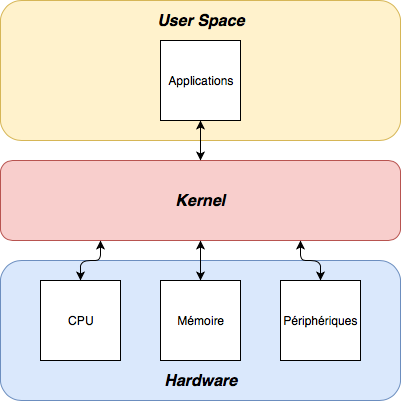
\includegraphics[scale=0.75]{images/kernel.png}
    \caption{Architecture du système d'exploitation}
    \label{os_arch}
\end{figure}

%%%%%%%%%%%%%%%%%%%%%%%%%%%%%%%%%%%%%%%%%%%%%%%%%%%%%%%%%%%%%%%%%%
%%%%%%%%%%%%%%%%%%%%%%%%%%%%%%%%%%%%%%%%%%%%%%%%%%%%%%%%%%%%%%%%%%

\subsection{Environnement de développement}
La machine utilisée pour le développement du projet est un MacBook Pro avec un
processeur Intel à 3 GHz. Il a quand même fallut utiliser une machine virtuelle
(VMware) utilisant Linux (Ubuntu 16.04.4 LTS) pour la compilation. Ce choix a été
fait car il existe beaucoup plus de documentation sur l'implémentation de systèmes
d'exploitation sur Linux que sur Mac. Bien que Mac \acrshort{os} soit un système
UNIX, les exécutables générés sur cet environnement n'ont pas le même format que
ceux générés sur Linux qui sont au format \acrshort{elf}. Ceci rend le développement
d'\acrshort{os} légèrement différent sur Mac \acrshort{os}. Linux est donc utilisé
pour la compilation et l'exécution du système d'exploitation. \\

Le code doit être compilé pour être exécutable sous une architecture \acrshort{IA-32}.
La compilation du code Rust est expliquée dans le chapitre \ref{rust_compil}. Certaines
parties du code du \textit{kernel} ont été écrites en assembleur car étant trop bas niveau
pour Rust. Nasm a été  utilisé pour compiler le code assembleur x86 en \acrshort{elf}
32 bits. Nasm produit des fichiers objets pouvant être liés à d'autres fichiers
objets (comme ceux générés par Rust) afin de créer un exécutable. Tout le mécanisme
de génération d'un \textit{kernel} exécutable est décrit en détail dans le chapitre
\ref{execution}. Pour ce projet, une machine virtuelle est utilisée pour démarrer
sur notre système d'exploitation. Cette machine virtuelle est QEMU. Elle peut
émuler plusieurs architectures dont l'architecture i386 qui nous intéresse ici.
QEMU peut démarrer un système d'exploitation depuis un fichier \acrshort{iso}
ou bien directement depuis un exécutable au format \acrshort{elf}. Dans notre
cas, un fichier \acrshort{iso} contenant le \textit{kernel} est généré.

\begin{figure}[!h]
    \centering
    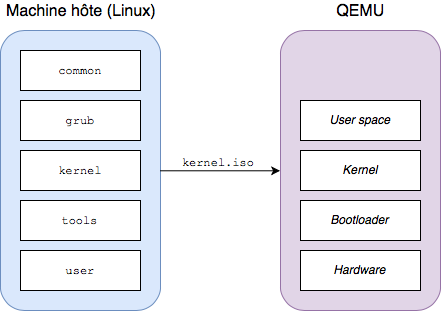
\includegraphics[scale=0.75]{images/global_arch.png}
    \caption{Architecture globale du projet}
    \label{os_arch}
\end{figure}

%%%%%%%%%%%%%%%%%%%%%%%%%%%%%%%%%%%%%%%%%%%%%%%%%%%%%%%%%%%%%%%%%%
%%%%%%%%%%%%%%%%%%%%%%%%%%%%%%%%%%%%%%%%%%%%%%%%%%%%%%%%%%%%%%%%%%

\newpage
\section{Langage Rust}
%%%%%%%%%%%%%%%%%%%%%%%%%%%%%%%%%%%%%%%%%%%%%%%%%%%%%%%%%%%%%%%%%%
%%%%%%%%%%%%%%%%%%%%%%%%%%%%%%%%%%%%%%%%%%%%%%%%%%%%%%%%%%%%%%%%%%

\subsection{Introduction}
Rust est un langage de programmation système développé par Mozilla et conçu pour
être sécurisé. Le but de Rust est de remplacer les autres langages système comme
le C ou le C++. Les trois caractéristiques mises en valeur par l'équipe de Rust
sont la rapidité, la sécurité (prévient des erreurs de segmentation) et la concurrence
(garantit la sûreté entre \textit{threads}) \cite{ref27}. La première version
de Rust est sortie en janvier 2012 \cite{ref28}. Ce langage est donc très récent
et emprunte beaucoup de concepts de programmation d'autres langages. Une première
partie de ce projet a été un travail de recherche afin d'apprendre ce langage.
Beaucoup de documentation est disponible sur le site de Rust dont le livre
de Rust, \textit{The Rust Programming Language}, sorti en deux éditions différentes
(\href{https://doc.rust-lang.org/book/first-edition}{\textit{First Edition}} et
\href{https://doc.rust-lang.org/book/second-edition}{\textit{Second Edition}}).
Ce livre est disponible en ligne et est une très bonne introduction au langage.
Il donne beaucoup d'exemples et permet rapidement de comprendre le fonctionnement de
Rust.

%%%%%%%%%%%%%%%%%%%%%%%%%%%%%%%%%%%%%%%%%%%%%%%%%%%%%%%%%%%%%%%%%%
%%%%%%%%%%%%%%%%%%%%%%%%%%%%%%%%%%%%%%%%%%%%%%%%%%%%%%%%%%%%%%%%%%

\subsection{Installation et compilation}
\subsubsection{Installation de Rust}
Rust est distribué sous trois versions différentes. La version \textit{stable},
la version \textit{beta} et la version \textit{nightly}. La version \textit{nightly}
possède plus de fonctionnalités mais sa stabilité n'est pas garantie. Cette version
a été utilisée pendant le développement du projet. Rustup est un gestionnaire de
version du langage Rust. Pour installer Rust ainsi que cet utilitaire, il faut
exécuter la commande suivante \cite{ref2}.

\begin{shellcode}
$ curl https://sh.rustup.rs -sSf | sh
\end{shellcode}

Le gestionnaire de version rustup peut maintenant être utilisé pour changer la
version de Rust. Notre système d'exploitation utilise la version \textit{nightly}
de Rust, la commande suivante doit donc être exécutée.

\begin{shellcode}
$ rustup override add nightly
\end{shellcode}

%%%%%%%%%%%%%%%%%%%%%%%%%%%%%%%%%%%%%%%%%%%%%%%%%%%%%%%%%%%%%%%%%%

\subsubsection{Compilation d'un programme en Rust}
\label{rust_compil}
Le compilateur de Rust est rustc. Il est installé automatiquement lors de
l'installation de Rust. Prenons le programme ci-dessous qui est contenu
dans le fichier \mintinline{text}{hello.rs}.

\begin{code}
\begin{rustcode}
fn main() {
    let hello = "Hello world!";
    println!("{}", hello);
}
\end{rustcode}
\caption{Premier programme en Rust}
\label{lst:rust:hello}
\end{code} \bigbreak

Le mot-clé \mintinline{rust}{let} indique qu'une variable est déclarée. On remarque
qu'aucun type n'est donné dans la déclaration. L'inférence de types est un des
nombreux concepts utilisés par Rust. L'équivalent en C serait
\mintinline{c}{char hello[] = "Hello world!"}. Le programme affiche ensuite cette
variable sur la sortie standard en utilisant la macro \mintinline{rust}{println!}.
Les macros seront vues plus en détail dans la suite de ce document. On peut les
distinguer des fonctions par la manière dont elles sont appelées. L'appel d'une
macro se fait avec son nom suivi d'un '!'. Ce programme affiche donc "Hello world!"
sur la sortie standard. Pour générer un exécutable à partir de ce code, le compilateur
de Rust, rustc peut être utilisé avec la commande \mintinline{shell}{rustc hello.rs}.
Cette méthode marche bien lorsqu'on ne veut compiler qu'un seul fichier
comme dans cet exemple. Cela devient vite compliqué lorsqu'il faut gérer des dépendences
entre plusieurs fichiers et utiiser des librairies externes. Heureusement,
une solution existe pour résoudre ce problème. Rust fournie un gestionnaire
de paquets nommé Cargo.

%%%%%%%%%%%%%%%%%%%%%%%%%%%%%%%%%%%%%%%%%%%%%%%%%%%%%%%%%%%%%%%%%%

\subsubsection{Cargo}
Le gestionnaire de paquets de Rust, Cargo, peut non seulement gérer les dépendences
d'un projet mais s'occupe aussi de sa compilation \cite{ref3}. Cargo est installé
en même temps que Rust, il n'y a donc pas de manipulations supplémentaires à faire
pour l'utiliser. Cargo fonctionne à l'aide d'un fichier de configuration du projet
au format \acrshort{toml}. Ce fichier doit être appelé \mintinline{text}{Cargo.toml}.
Le contenu du fichier \mintinline{text}{Cargo.toml} ressemble généralement
au code dans le \textit{listing} \ref{lst:rust:cargotoml} \cite{ref2}.

\begin{code}
\begin{minted}[fontsize=\footnotesize,tabsize=4,frame=single,linenos]{text}
[package]
name = "hello"
version = "0.1.0"
authors = ["Your Name <you@example.com>"]

[dependencies]
\end{minted}
\caption{Contenu du fichier \mintinline{text}{Cargo.toml}}
\label{lst:rust:cargotoml}
\end{code} \bigbreak

Cargo compile et gère automatiquement les dépendences de tous les fichiers contenus
dans le répertoire \mintinline{text}{src}. Si on reprend l'exemple du \textit{listing}
\ref{lst:rust:hello}, un projet utilisant Cargo aurait l'arborescence suivante. \\

\dirtree{%
.1 \mintinline{text}{hello}.
.2 \mintinline{text}{Cargo.toml}.
.2 \mintinline{text}{src}.
.3 \mintinline{text}{main.rs}.
} \bigbreak

Des dépendences externes (appelées \textit{crates}) peuvent être utilisées dans
le projet en les ajoutant dans le fichier \acrshort{toml}, sous la section \textit{dependencies}.
Une \textit{crate} peut être en local sur la machine hôte ou être disponible en ligne
sur \href{https://crates.io}{Crate.io}. Ce site sert de registre pour toutes les
librairies Rust développées par la communauté. Cargo télécharge automatiquement
les dépendences depuis \href{https://crates.io}{Crate.io} \cite{ref2}. Pour compiler un projet,
rustc n'a plus a être utilisé. Cargo fait appelle au compilateur
de rust lui même. Pour demander à cargo de compiler le projet il faut exécuter
la commande \mintinline{shell}{cargo build}. Si le projet est un exécutable,
il est lancé avec la commande \mintinline{shell}{cargo run}. Notre système
d'exploitation utilise un gestionnaire de paquets basé sur Cargo. Celui-ci
se nomme Xargo. Il peut être installé directement depuis Cargo en utilisant
la commande \mintinline{shell}{cargo install xargo}. Xargo est fait pour compiler
un projet Rust dans un environnement \textit{bare metal}. Dans ce type d'environnement
il n'y a aucune librairie système étant donné que nous créons nous même le système.
Le code doit donc être compilé sans dépendences à la librairie standard. Rust a tout
de même besoin d'une base pour être compilé. Cette base est fournie par la librairie
\mintinline{rust}{core}. Xargo lie la librairie \mintinline{rust}{core} au projet
automatiquement contrairement à Cargo \cite{ref8}.

%%%%%%%%%%%%%%%%%%%%%%%%%%%%%%%%%%%%%%%%%%%%%%%%%%%%%%%%%%%%%%%%%%

\subsubsection{Compilation croisée}
Dans le cadre du projet, le code Rust a du être compilé pour une architecture
Intel 32-bits (\acrshort{IA-32}). On parle ici de compilation croisée
car une machine hôte (le \textit{host} en anglais) compile du code pour une
machine cible (la \textit{target} en anglais). Quand on fait de la compilation
croisée, on se réfère à des caractèristiques nommées \textit{triple}. Un \textit{triple}
a généralement le format architecture-vendeur-système-\acrshort{abi}. Par exemple
pour \textit{cross-compiler} pour une machine Apple, le format du \textit{triple}
est x86$\_$64-apple-darwin. A noter que l'\acrshort{abi} n'est pas spécifiée.
Rust propose un système natif de compilation croisée pour de nombreuses cibles.
Ceci peut se faire avec le compilateur rustc ou bien avec Cargo en spécifiant
la machine cible avec l'option \mintinline{shell}{--target=} suivie du
\textit{target triple}. Il est possible de configurer son propre \textit{target triple}
dans un fichier \acrshort{json} placé à la racine du projet. Dans ce cas, il
faut donner le nom du fichier (sans l'extension .json) à l'option de Cargo.
Dans notre \acrshort{os}, le nom du fichier est \mintinline{text}{i386-rust_os.json}.
Notre projet a donc l'arborescence suivante. \\

\dirtree{%
.1 \mintinline{text}{kernel}.
.2 \mintinline{text}{Cargo.toml}.
.2 \mintinline{text}{i386-rust_os.json}
.2 \mintinline{text}{src}.
.3 \mintinline{text}{kernel.rs}.
} \bigbreak

Le fichier \mintinline{text}{i386-rust_os.json} configure la machine cible
sous architecture i386 (\acrshort{IA-32}) et sans système d'exploitation.
Ci-dessous, le contenu de ce fichier. \\

\begin{code}
\begin{minted}[fontsize=\footnotesize,tabsize=4,frame=single,linenos]{text}
{
  "llvm-target": "i386-unknown-none",
  "data-layout": "e-m:e-p:32:32-f64:32:64-f80:32-n8:16:32-S128",
  "linker-flavor": "gcc",
  "target-endian": "little",
  "target-pointer-width": "32",
  "target-c-int-width": "32",
  "arch": "x86",
  "os": "none",
  "disable-redzone": true,
  "features": "-mmx,-sse,+soft-float",
  "panic-strategy": "abort"
}
\end{minted}
\caption{Contenu du fichier \mintinline{text}{i386-rust_os.json}}
\label{lst:rust:target}
\end{code} \bigbreak

Tous les champs du \textit{target triple} sont décrits dans la documentation de
Rust \cite{ref4}. Le contenu de ce fichier est inspiré de plusieurs \textit{target triples}
trouvés sur le \textit{net}. L'un dans une \textit{issue} du \textit{repository}
de Rust sur GitHub \cite{ref5} et l'autre dans un blog parlant de l'écriture
d'un système d'exploitation en Rust \cite{ref8}. La compilation croisée de notre
\textit{kernel} peut maintenant se faire avec la commande
\mintinline{shell}{xargo build --target=i386-rust_os}. A noter qu'il existe un
\textit{bug} avec l'option \mintinline{text}{target} quand on utilise notre propre
\textit{target triple} \cite{ref7}. Pour ne pas qu'il se produise, il faut indiquer
le chemin d'accès au répertoire contenant le fichier \acrshort{json} en utilisant
la variable d'environnement \mintinline{shell}{RUST_TARGET_PATH}. La commande finale
pour compiler le projet est la suivante.

\begin{shellcode}
$ RUST_TARGET_PATH=$(pwd) xargo build --target i386-rust_os
\end{shellcode}

%%%%%%%%%%%%%%%%%%%%%%%%%%%%%%%%%%%%%%%%%%%%%%%%%%%%%%%%%%%%%%%%%%
%%%%%%%%%%%%%%%%%%%%%%%%%%%%%%%%%%%%%%%%%%%%%%%%%%%%%%%%%%%%%%%%%%

\subsection{Bases du langage}
\subsubsection{Commentaires}
Les commentaires en Rust ont la même syntaxe que les commentaires en C. Le \textit{listing}
\ref{lst:rust:comments} montre les différents types de commentaire.

\begin{code}
\begin{rustcode}
// Commentaire sur une seule ligne

/* Commentaire sur
   plusieurs lignes */
\end{rustcode}
\caption{Commentaires en Rust}
\label{lst:rust:comments}
\end{code} \bigbreak

%%%%%%%%%%%%%%%%%%%%%%%%%%%%%%%%%%%%%%%%%%%%%%%%%%%%%%%%%%%%%%%%%%

\subsubsection{Variables et mutabilité}
Les variables en Rust sont toutes constantes par défaut. Le code du \textit{listing}
\ref{lst:rust:var1} ne pourra pas compiler.

\begin{code}
\begin{rustcode}
let x = 0;
x += 1; // Erreur !
\end{rustcode}
\caption{Exemple de variable immutable}
\label{lst:rust:var1}
\end{code} \bigbreak

Pour rendre une variable mutable, le mot-clé \mintinline{rust}{mut} doit être utilisé.
Le code du \textit{listing} \ref{lst:rust:var2} corrige celui du \textit{listing}
\ref{lst:rust:var1}.

\begin{code}
\begin{rustcode}
let mut x = 0;
x += 1; // Plus d'erreur, la variable x est mutable
\end{rustcode}
\caption{Exemple de variable mutable}
\label{lst:rust:var2}
\end{code} \bigbreak

Une variable peut aussi être réécrite. On appelle ça le \textit{shadowing}.

\begin{code}
\begin{rustcode}
let x = 0;
let x = "zero";
\end{rustcode}
\caption{Exemple de \textit{shadowing}}
\label{lst:rust:var3}
\end{code} \bigbreak

Le mot-clé \mintinline{rust}{let} sans \mintinline{rust}{mut} peut faire penser
aux constantes en C. Rust permet aussi de déclarer des constantes avec le mot-clé
\mintinline{rust}{const}. Lors d'une déclaration de constante en Rust, le type
de la variable doit être donné ainsi que sa valeur qui doit être constante (valeur
fixée à la compilation et non au \textit{runtime}). Une constante est déclarée
globalement. Pour déclarer une variable globalement il faut utiliser le mot-clé
\mintinline{rust}{static}. Comme pour les constantes, quand une variable est déclarée
statiquement, son type et sa valeur doivent être déterminés à la compilation.

\begin{code}
\begin{rustcode}
const KHEAP_SIZE        : usize = 0x1000000;
static mut KHEAP_ADDR   : u32   = 0;
\end{rustcode}
\caption{Déclaration d'une constante et d'une variable statique}
\label{lst:rust:var4}
\end{code} \bigbreak

%%%%%%%%%%%%%%%%%%%%%%%%%%%%%%%%%%%%%%%%%%%%%%%%%%%%%%%%%%%%%%%%%%

\subsubsection{Fonctions et macros}
Les fonctions en Rust sont semblables aux fonctions en C. Leur déclaration se fait
avec le mot-clé \mintinline{rust}{fn}. Les macros de Rust reprennent le concept
des macros du langage C. La différence entre une macro et une fonction est qu'une
macro va être remplacée à la compilation par le code qu'elle contient. De plus,
le nombre d'arguments d'une macro n'est pas fixe. Une macro fonctionne par motifs.
Prenons pour exemple l'implémentation de la macro \mintinline{rust}{println!}. \\

\begin{code}
\begin{rustcode}
macro_rules! println {
    () => (print!("\n"));
    ($fmt:expr) => (print!(concat!($fmt, "\n")));
    ($fmt:expr, $($arg:tt)*) => (print!(concat!($fmt, "\n"), $($arg)*));
}
\end{rustcode}
\caption{Code source de la macro \mintinline{rust}{println!}}
\label{lst:rust:macro}
\end{code} \bigbreak

Cette macro a trois motifs différents. Si aucun argument est donné à la macro,
le premier motif va être utilsé. Nous pouvons voir qu'il affiche simplement
un saut de ligne avec la macro \mintinline{rust}{print!}. Dans une macro, la partie gauche
contient un ensemble de symboles et la partie droite l'action à effectuer avec
les symboles. Prenons maintenant la deuxième ligne de cette macro. Pour que
ce motif soit appelé, une expression doit être donnée à la macro. Le symbole
de cette expression est \mintinline{rust}{$fmt} (comme le nom d'un argument dans
une fonction, le symbole d'une macro est arbitraire). Ce \textit{pattern} est
appelé quand par exemple nous ne voulons afficher qu'une chaîne de caractères
non formatée (\mintinline{rust}{println!("Hello")}). La dernière ligne de cette
macro représente le cas où un ou plusieurs arguments suplémentaires sont donnés
à la macro. Dans cet exemple, c'est le cas où on veut formater la chaîne de caractères
comme dans le \textit{listing} \ref{lst:rust:hello}. Quand un symbole est suivi
d'un '*', cela veut dire qu'il peut être répété zéro ou plus de fois \cite{ref1}.

%%%%%%%%%%%%%%%%%%%%%%%%%%%%%%%%%%%%%%%%%%%%%%%%%%%%%%%%%%%%%%%%%%

\subsubsection{Structures de contrôle}
Le langage Rust propose les mêmes structures de contrôle que le langage C.
Une condition se fait avec l'expression \mintinline{rust}{if} et du code
peut être répété avec les expressions  \mintinline{rust}{for},  \mintinline{rust}{while}
et  \mintinline{rust}{loop}. Rust possède aussi une structure de contrôle pour
faire du \textit{pattern matching}. Elle est utilisée avec l'expression \mintinline{rust}{match}.
A noter qu'on parle ici d'expression. Une expression peut être utilisée dans la
déclaration d'une variable. Le code suivant est donc possible \cite{ref2}. \\

\begin{code}
\begin{rustcode}
let condition = true;
let number = if condition {
    5
} else {
    6
};
\end{rustcode}
\caption{Utiliser l'expression \mintinline{rust}{if} dans une déclaration de variable}
\label{lst:rust:if}
\end{code} \bigbreak

Dans cet exemple, la variable \mintinline{rust}{number} sera initialisée à la
valeur 5. \newpage

%%%%%%%%%%%%%%%%%%%%%%%%%%%%%%%%%%%%%%%%%%%%%%%%%%%%%%%%%%%%%%%%%%

\subsubsection{Structures de données}
Rust donne aussi accès à des structures de données, semblables aux structures
C dans leur déclaration mais tout de même différentes. Ces structures peuvent
implémenter des méthodes. On peut donc aussi les comparer aux classes en Java.
Ci-dessous, une structure implémentant deux méthodes.

\begin{code}
\begin{rustcode}
#[derive(Clone)]
#[repr(C, align(4096))]
pub struct PageTable {
    pub entries: [u32;0x400]
}
impl PageTable {
    fn null() -> PageTable {
        PageTable {
            entries: [0;0x400]
        }
    }
    pub fn as_ptr(&mut self) -> u32 {
        self as *const PageTable as u32
    }
}
\end{rustcode}
\caption{Exemple de structure en Rust}
\label{lst:rust:struct}
\end{code} \bigbreak

Ici, la structure \mintinline{rust}{PageTable} ne contient qu'un seul champs
mais il peut y en avoir plus. Les deux lignes commençant par un '\#' sont des attributs
appliqués à la structure \cite{ref2}. Le premier attributs permet d'inclure automatiquement
les fonctionnalités du trait \mintinline{rust}{Clone} à notre structure. Le deuxième attribut
indique que cette structure doit être représentée comme en C dans la mémoire et
être alignée sur 4096 octets. L'implémentation de méthodes pour une structure se
fait avec le mot-clé \mintinline{rust}{impl}. La première méthode est un constructeur
renvoyant simplement une structure initialisée avec des 0. La deuxième méthode peut
être appliquée à une structure, elle renvoie l'adresse de cette dernière. Le \textit{listing}
\ref{lst:rust:struct:methods} montre comment appeler ces méthodes.

\begin{code}
\begin{rustcode}
let table = PageTable::null();
let table_addr = table.as_ptr();
\end{rustcode}
\caption{Appels aux méthodes d'une structure}
\label{lst:rust:struct:methods}
\end{code} \bigbreak

A noter que le mot-clé \mintinline{rust}{pub} est utilisé à trois reprises dans
le \textit{listing} \ref{lst:rust:struct}. Ce mot-clé contrôle la visibilité de
la variable, la fonction, le champs ou la structure qui lui est associé. Il fait
le contraire du mot-clé \mintinline{java}{private} en Java (de base tout est privé
dans un fichier Rust) \cite{ref2}. En plus des structures, Rust propose aussi
les énumérations ou \mintinline{rust}{enum}. Un \mintinline{rust}{enum} permet
de définir un type en énumérant toutes ses valeurs possibles \cite{ref2}. Le
\textit{listing} \ref{lst:rust:enum} donne un exemple d'\mintinline{rust}{enum}
dont chaque valeur est sur huit bits.

\begin{code}
\begin{rustcode}
#[repr(u8)]
pub enum Color {
    Black = 0x0,
    White = 0xf
}
\end{rustcode}
\caption{Déclaration d'un \mintinline{rust}{enum}}
\label{lst:rust:enum}
\end{code} \bigbreak

%%%%%%%%%%%%%%%%%%%%%%%%%%%%%%%%%%%%%%%%%%%%%%%%%%%%%%%%%%%%%%%%%%
%%%%%%%%%%%%%%%%%%%%%%%%%%%%%%%%%%%%%%%%%%%%%%%%%%%%%%%%%%%%%%%%%%

\subsection{Spécificités du langage}
\subsubsection{\textit{Ownership} et références}
L'\textit{Ownership} est la fonctionnalité de Rust lui permettant de garantir la
sécurité au niveau de la mémoire. Elle est décrite dans le livre de Rust comme
la fonctionnalité fondamentale du langage. Chaque valeur en Rust est liée à une
variable qui est appelée son propriétaire (\textit{owner} en anglais). Une valeur
ne peut avoir qu'un seul propriétaire à la fois. Quand on sort de la portée de
la variable, la valeur n'est plus accessible \cite{ref2}. Prenons pour exemple
la structure \mintinline{rust}{PageTable} décrite plus haut. Le code suivant
provoquera une erreur.

\begin{code}
\begin{rustcode}
let table1 = PageTable::null();
let table2 = table1;              // table2 prend l'ownership de la valeur de table1
let table_addr = table1.as_ptr(); // Erreur ! table1 n'a plus de valeur
\end{rustcode}
\caption{Changement d'\textit{ownership}}
\label{lst:rust:ownership}
\end{code} \bigbreak

Pour corriger cette erreur, il faut copier la valeur de la variable \mintinline{rust}{table1}
dans \mintinline{rust}{table2} en utilisant la méthode \mintinline{rust}{clone()}.
C'est pour cette raison que nous avons spécifié l'utilisation des fonctionnalités
du trait \mintinline{rust}{Clone} lors de la déclaration de la structure dans
le \textit{listing} \ref{lst:rust:struct}. Notre variable peut être stockée sur
la pile car sa taille est connue à la compilation. Un autre trait
offert par Rust peut être utilisé ici pour copier sa valeur. C'est le trait
\mintinline{rust}{Copy}. Les fonctionnalités de ce trait
peuvent être rajouté à une structure stockée dans la pile en l'ajoutant à l'attribut
\mintinline{rust}{derive}. Grâce à ce trait, il n'y a pas besoin
d'appeler la méthode \mintinline{rust}{clone()} pour copier la valeur. La copie
est faite automatiquement. Pour ne pas perdre l'\textit{Ownership} lors du passage
d'une variable à une fonction, une référence à cette variable peut être donnée
à la place (opérateurs \mintinline{rust}{&} et \mintinline{rust}{&mut}) \cite{ref2}.

%%%%%%%%%%%%%%%%%%%%%%%%%%%%%%%%%%%%%%%%%%%%%%%%%%%%%%%%%%%%%%%%%%

\subsubsection{Traits}
Un trait en Rust ajoute des fonctionnalités à un type.
Ces fonctionnalités peuvent être partagées entre plusieurs types. Il existe des
traits déjà disponibles dans le code de Rust comme ceux
utilisés précédemment (\mintinline{rust}{Clone} et \mintinline{rust}{Copy}).
Un trait est déclaré avec le mot-clé \mintinline{rust}{trait}. Pour implémenter
un trait dans une structure, le mot-clé \mintinline{rust}{impl} peut aussi
être utilisé. Reprenons la structure \mintinline{rust}{PageTable} du \textit{listing}
\ref{lst:rust:struct}. Cette structure contient un tableau et il serait pratique
de pouvoir récupérer un élément de ce tableau directement en faisant
\mintinline{rust}{table[i]} avec \mintinline{rust}{i} contenant l'indice du tableau.
Actuellement, ce n'est pas possible, il faut faire \mintinline{rust}{table.entries[i]}.
Les traits \mintinline{rust}{Index} et \mintinline{rust}{IndexMut} permettent
ce comportement. Le \textit{listing} \ref{lst:rust:traits} montre comment implémenter
ces traits dans le cas de \mintinline{rust}{PageTable}.

\begin{code}
\begin{rustcode}
impl Index<usize> for PageTable {
    type Output = u32;
    fn index(&self, index: usize) -> &u32 {
        &self.entries[index]
    }
}
impl IndexMut<usize> for PageTable {
    fn index_mut(&mut self, index: usize) -> &mut u32 {
        &mut self.entries[index]
    }
}
\end{rustcode}
\caption{Implémentation de traits pour une structure}
\label{lst:rust:traits}
\end{code}

%%%%%%%%%%%%%%%%%%%%%%%%%%%%%%%%%%%%%%%%%%%%%%%%%%%%%%%%%%%%%%%%%%

\subsubsection{Gestion des erreurs}
Rust possède tout un mécanisme de gestion des erreurs. Les erreurs sont séparées
en deux catégories, les erreurs récupérables et non récupérables. Quand une erreur
est récupérable, le type \mintinline{rust}{Result<T, E>} est utilisé pour gérer
l'erreur (en général dans une expression \mintinline{rust}{match}). Dans le cas
contraire, la macro \mintinline{rust}{panic!} est appelée. Par défaut quand, un
programme panique, Rust réinitialise la pile et nettoie la mémoire avant de quitter.
Ce comportement peut être annulé en rajoutant la section du \textit{listing}
\ref{lst:rust:errors:abort} \cite{ref2}.

\begin{code}
\begin{minted}[fontsize=\footnotesize,tabsize=4,frame=single,linenos]{text}
[profile.release]
panic = 'abort'
\end{minted}
\caption{Section à ajouter au fichier \acrshort{toml}}
\label{lst:rust:errors:abort}
\end{code} \bigbreak

\subsubsection{Tests unitaires}
Rust offre tout un mécanisme des tests unitaires. Ce mécanimse est utilisé avec
Cargo en exécutant la commande \mintinline{shell}{cargo test}. Quand cette
commande est exécutée, Cargo cherche le module \mintinline{rust}{tests} du projet.
Un module en Rust contient des variables, des fonctions et des structures. Il permet
de diviser le code en plus petites parties. Un module peut être dans le fichier
principal du projet ou dans un fichier différent. Dans le cas des tests unitaires
un module basique ressemblerait à celui décrit dans le \textit{listing} suivant.

\begin{code}
\begin{rustcode}
#[cfg(test)]
mod tests {
    #[test]
    fn it_works() {
        assert_eq!(2 + 2, 4);
    }
}
\end{rustcode}
\caption{Module \mintinline{rust}{tests}}
\label{lst:rust:tests}
\end{code} \bigbreak

L'attribut \mintinline{rust}{#[cfg(test)]} dit à Rust de ne compiler le code
que si \mintinline{text}{cargo test} est exécuté. Lors de l'exécution des tests
unitaires, Cargo appelle toutes les fonctions préfixées de l'attribut \mintinline{rust}{test}
\cite{ref2}. Malheureusement, les tests unitaires n'ont pas pu être beaucoup utilisés
dans le cadre de ce projet car ils sont exécutés sur la machine hôte. Notre système
d'exploitation est compilé sur la machine hôte mais est exécuté sur une autre
machine (dans notre cas une machine virtuelle, QEMU). Il n'est donc pas possible
d'utiliser ce mécanisme de tests pour tester les différentes parties du système.

%%%%%%%%%%%%%%%%%%%%%%%%%%%%%%%%%%%%%%%%%%%%%%%%%%%%%%%%%%%%%%%%%%

\subsubsection{\textit{Unsafe} Rust}
Nous avons vu que Rust garantit la sécurité de la mémoire à la compilation.
Le compilateur ne nous laisse par exemple pas déréférencer un pointeur, modifier
une variable statique ou encore appeler du code d'un autre langage.
Le problème est que nous utilisons Rust dans le cadre de la programmation système.
Rust est utilisé dans ce projet pour créer un système d'exploitation. Il est nécéssaire
d'accéder à la mémoire sans restrictions et d'appeler du code assembleur. Rust donne
la possibilité de supprimer la protection du compilateur avec le mot-clé
\mintinline{rust}{unsafe}. Quand un code est \mintinline{rust}{unsafe}, plus aucune
protection n'est appliquée il est donc très déconseillé de l'utiliser. En effet,
en utilisant du code \mintinline{rust}{unsafe}, on perd beaucoup d'avantages de Rust
\cite{ref2}.

%%%%%%%%%%%%%%%%%%%%%%%%%%%%%%%%%%%%%%%%%%%%%%%%%%%%%%%%%%%%%%%%%%
%%%%%%%%%%%%%%%%%%%%%%%%%%%%%%%%%%%%%%%%%%%%%%%%%%%%%%%%%%%%%%%%%%

\newpage
\section{Exécution du \textit{kernel}}
%%%%%%%%%%%%%%%%%%%%%%%%%%%%%%%%%%%%%%%%%%%%%%%%%%%%%%%%%%%%%%%%%%
%%%%%%%%%%%%%%%%%%%%%%%%%%%%%%%%%%%%%%%%%%%%%%%%%%%%%%%%%%%%%%%%%%

\subsection{Compilation}
Quand on veut compiler un simple code C en utilisant \acrshort{gcc} par
exemple, le compilateur passe par plusieurs étapes. Le préprocesseur génère d'abord
un fichier C en fonction des directives de préprocesseur. Ce fichier C est ensuite
compilé en code assembleur qui est lui même compilé en code objet. Le \textit{linker}
permet ensuite de lier les différents fichiers objets et générer un exécutable.
Nous avons déjà eu un aperçu des différentes étapes de la compilation d'un \acrshort{os}
de type \textit{bare metal} dans la partie 3.2. A la différence de la compilation
d'un code C, nous avons d'un côté du code assembleur et de l'autre du code Rust.
Nasm et cargo permettent tous deux de générer des fichiers objets. Il n'y a donc
que la dernière étape à effectuer ce que \acrshort{gcc} permet de faire avec
la commande suivante.
\begin{minted}[tabsize=4]{shell}
gcc $(OBJS) -T $(LINKER) -static -m32 -ffreestanding -nostdlib -o $@ $(RUST)
\end{minted}
Ici, \mintinline{shell}{$(OBJS)} représente les fichiers objets générés par
\mintinline{rust}{nasm}, \mintinline{shell}{$(LINKER)} est un fichier permettant
de faire l'édition des liens et \mintinline{shell}{$(RUST)} représente les fichiers
objets générés par Rust.\cite{ref42}

%%%%%%%%%%%%%%%%%%%%%%%%%%%%%%%%%%%%%%%%%%%%%%%%%%%%%%%%%%%%%%%%%%
%%%%%%%%%%%%%%%%%%%%%%%%%%%%%%%%%%%%%%%%%%%%%%%%%%%%%%%%%%%%%%%%%%

\subsection{\textit{Linking}}
Nous avons vu dans la partie précédente que \acrshort{gcc} a besoin d'un fichier
pour faire l'édition des liens. Si ce fichier n'est pas donné, il en utilise un par
défaut. Le \textit{linker} permet de structurer le code par sections. Prenons
pour exemple le \textit{script} utilisé pour ce projet.

\begin{minted}[fontsize=\footnotesize,linenos,frame=single,tabsize=4]{c}
ENTRY(entrypoint)
SECTIONS {
  . = 1M;
  .boot ALIGN(4):
  {
    *(.multiboot)
  }
  .stack ALIGN(4):
  {
    *(.stack)
  }
  .text ALIGN(4K) :
  {
    *(.text*)
  }
  .rodata ALIGN(4K) :
  {
    *(.rodata*)
  }
  .data ALIGN(4K) :
  {
    *(.data*)
  }
  .bss ALIGN(4K) :
  {
    *(COMMON)
    *(.bss*)
  }
}
\end{minted}

L'appel à \mintinline{c}{ENTRY} permet de spécifier l'entrée du \textit{kernel}.
Pour un simple programme en C l'entrée serait le \textit{main}. Ici, ce sera
l'entrée de notre \textit{kernel} donc la première fonction exécutée au \textit{boot}.
\mintinline{text}{SECTION} va dire au linker où placer les parties du code. Par exemple, 
la section \mintinline{text}{.text} contiendra le code et la section \mintinline{text}{.data}
contiendra les variables initialisées \cite{ref42,ref9,ref10,ref11}. Voici donc la structure
du fichier \acrshort{elf} qui serait généré à l'aide de ce \textit{script}.

\begin{figure}[!h]
  \centering
  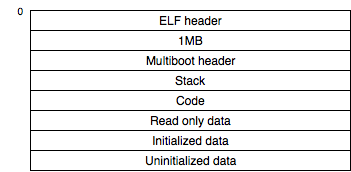
\includegraphics[scale=0.75]{images/elf_struct.png}
  \caption{Strucutre du fichier \acrshort{elf}}
\end{figure}

A noter que les sections commencent avec un \textit{offset} de 1MB. Nous avons eu
besoin de faire ça car les premiers 1MB dans un \acrshort{os} sont reservés \cite{ref42,ref13}.
La mémoire vidéo (\acrshort{vram}) se situe par exemple dans cette zone.

%%%%%%%%%%%%%%%%%%%%%%%%%%%%%%%%%%%%%%%%%%%%%%%%%%%%%%%%%%%%%%%%%%
%%%%%%%%%%%%%%%%%%%%%%%%%%%%%%%%%%%%%%%%%%%%%%%%%%%%%%%%%%%%%%%%%%

\subsection{\textit{Boot}}
\subsubsection{Principe général}
Quand un ordinateur est allumé, un signal est envoyé à la carte mère qui démarre
l'alimentation. Le processeur démarre alors en mode 16-bits. Le signal "Power Ok"
est envoyé au \acrshort{bios} qui est le \textit{firmware} du \acrshort{pc}
(localisé en mémoire flash de la carte mère). Le \acrshort{bios} initialise alors
la séquence POST (\textit{Power On Self Test}) qui vérifie que chaque périphérique
est alimenté et que la mémoire est ok puis initialise chaque périphérique et enfin
redonne la main au \acrshort{bios} qui continue le \textit{boot}. Le \acrshort{bios}
charge ensuite les 512 premiers bytes (\acrshort{mbr}) du premier disque qui doit
charger le \textit{kernel} en mémoire et l'exécuter. Pour résumer, le \textit{boot}
d'une machine à base de \acrshort{bios} se déroule de la manière ci-dessous.\cite{ref42}

\begin{figure}[!h]
  \centering
  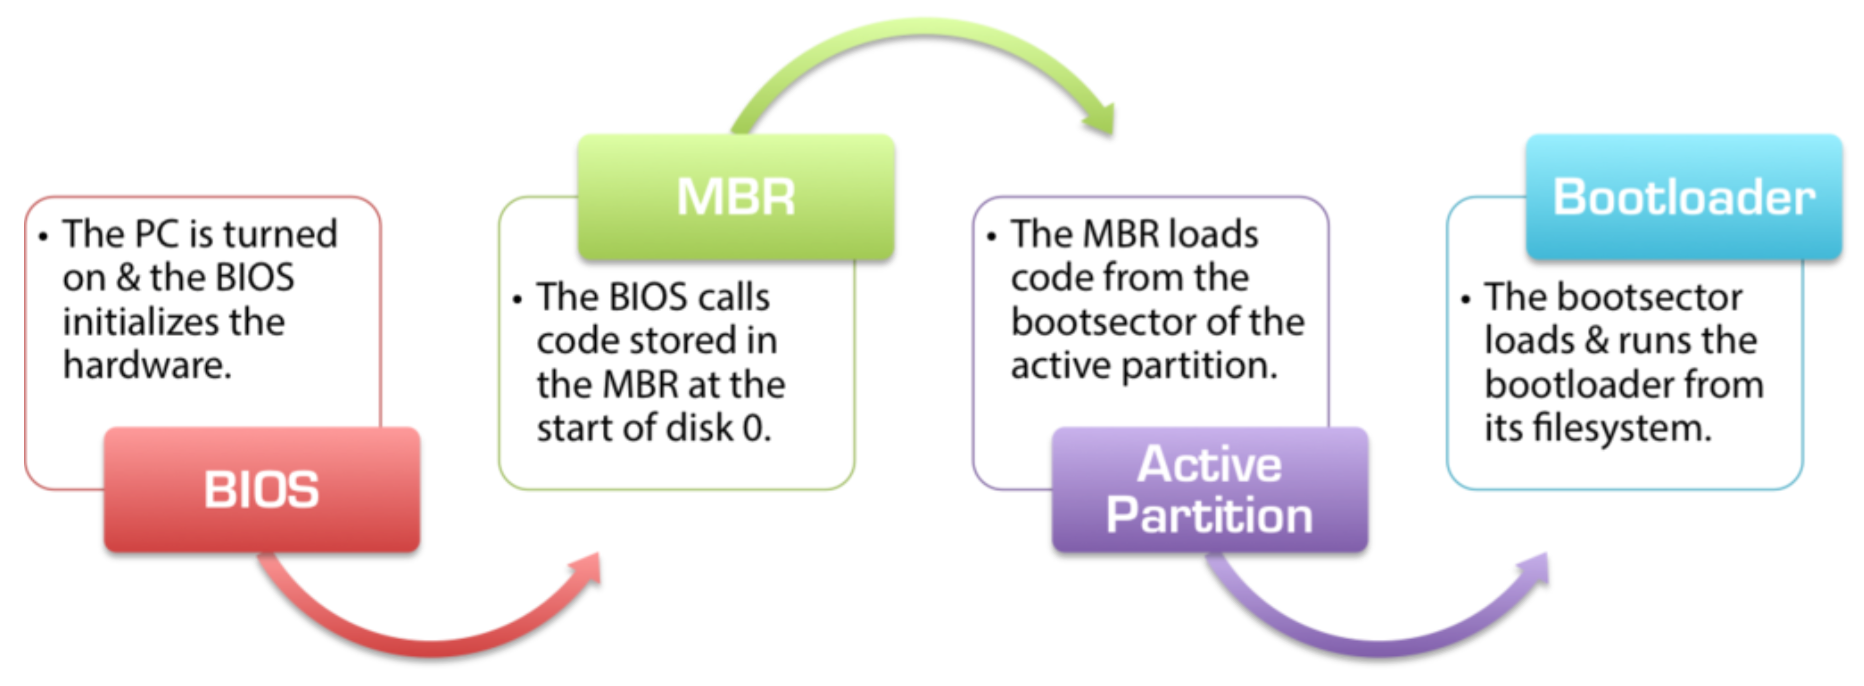
\includegraphics[scale=0.4]{images/bios_boot.png}
  \caption{\textit{Boot} d'une machine à base de \acrshort{bios}}
\end{figure}

%%%%%%%%%%%%%%%%%%%%%%%%%%%%%%%%%%%%%%%%%%%%%%%%%%%%%%%%%%%%%%%%%%

\subsubsection{\acrshort{grub}}
Le \acrshort{mbr} contient ce qui est appelé le \textit{bootloader}. Le \textit{bootloader}
est le morceau de code qui va charger le \textit{kernel} en mémoire et l'exécuter.
C'est ici qu'entre en scène \acrshort{grub}. \acrshort{grub} est un \textit{bootloader}
puissant et versatile permettant de charger n’importe quel type de système d’exploitation.
Son initialisation se fait par étapes.
\begin{itemize}[label=\textbullet]
	\item \textit{Stage} 1: Chargé en mémoire par le \acrshort{bios} depuis le
    \acrshort{mbr}, il contient le code pour charger le \textit{Stage} 1.5
	\item \textit{Stage} 1.5: Chargé en mémoire par le \textit{Stage} 1, il contient
    les drivers nécessaires à l'accès au système de fichiers par le \textit{Stage} 2
	\item \textit{Stage} 2: Chargé en mémoire par le \textit{Stage} 1.5, il affiche
    le menu de \acrshort{grub}. Il permet de sélectionner et charger un \acrshort{os}
\end{itemize}

\acrshort{grub} permet de charger n'importe quel type de système d'exploitation
grace au standard \textit{Multiboot}. Ce standard permet à tout \textit{bootloader}
de charger tout \acrshort{os} compatible \cite{ref42,ref12}.

\subsubsection{Image \acrshort{iso}}
Nous avons déjà pu voir que le \textit{boot} du \textit{kernel} se faisait à partie
d'une image \acrshort{iso} dans la partie 3.2.4. Pour qu'une image \acrshort{iso}
soit \textit{bootable}, il est nécessaire que \acrshort{grub} soit installé dans
les huit premiers KB du disque. Prenons l'arborescence suivante :

\begin{minted}[tabsize=4]{shell}
isofiles
└── boot
    └── grub
\end{minted}

Les fichiers \mintinline{text}{kernel.elf} (kernel sur lequel nous voulons
\textit{booter}), \mintinline{text}{menu.lst} (fichier de configuration de \acrshort{grub})
et \mintinline{text}{stage2_eltorito} doivent être copiés de manière à obtenir
l'arborescence suivante :

\begin{minted}[tabsize=4]{text}
isofiles
└── boot
    ├── grub
    │   ├── menu.lst
    │   └── stage2_eltorito
    └── kernel.elf
\end{minted}

Pour finir, il faut exécuter la commande :
\begin{minted}[tabsize=4]{shell}
genisoimage -R -b boot/grub/stage2_eltorito -input-charset utf8 -no-emul-boot \
-boot-info-table -o os.iso isofiles
\end{minted}
Cette commande génerera une image \acrshort{iso} \textit{bootable} nommée \mintinline{text}{os.iso}\cite{ref42}.

%%%%%%%%%%%%%%%%%%%%%%%%%%%%%%%%%%%%%%%%%%%%%%%%%%%%%%%%%%%%%%%%%%
%%%%%%%%%%%%%%%%%%%%%%%%%%%%%%%%%%%%%%%%%%%%%%%%%%%%%%%%%%%%%%%%%%

\newpage
\section{Gestion mémoire}
%%%%%%%%%%%%%%%%%%%%%%%%%%%%%%%%%%%%%%%%%%%%%%%%%%%%%%%%%%%%%%%%%%
%%%%%%%%%%%%%%%%%%%%%%%%%%%%%%%%%%%%%%%%%%%%%%%%%%%%%%%%%%%%%%%%%%

\subsection{Introduction}
Le système d'exploitation développé est exécuté sur une architecture \acrshort{IA-32}
(Intel 32-bits) aussi appelée i386. La mémoire est donc adressée sur 32 bits.
$2^{32}=4Go$, on peut en déduire que la taille totale de la mémoire adressable est
de 4Go dans notre système d'exploitation. Avoir un espace adressable de 4Go ne veut
pas forcément dire que la mémoire physique (\acrshort{ram}) est de 4Go aussi. En
réalité, la taille de la \acrshort{ram} dépend du \textit{hardware}. Dans notre
cas le matériel est émulé par QEMU. La taille de la mémoire physique de notre \acrshort{os}
dépend de la configuration de l'émulateur. Ces 4Go sont donc virtuels. Lorsqu'une
tache est exécutée, elle est chargée en mémoire et est définie par la paire base
et limite. La base est son adresse physique dans la \acrshort{ram} et la limite
est sa taille. La figure \ref{ex_base_limit} donne un exemple d'adressage de plusieurs
processus \cite{ref42}.

\begin{figure}[!h]
  \centering
  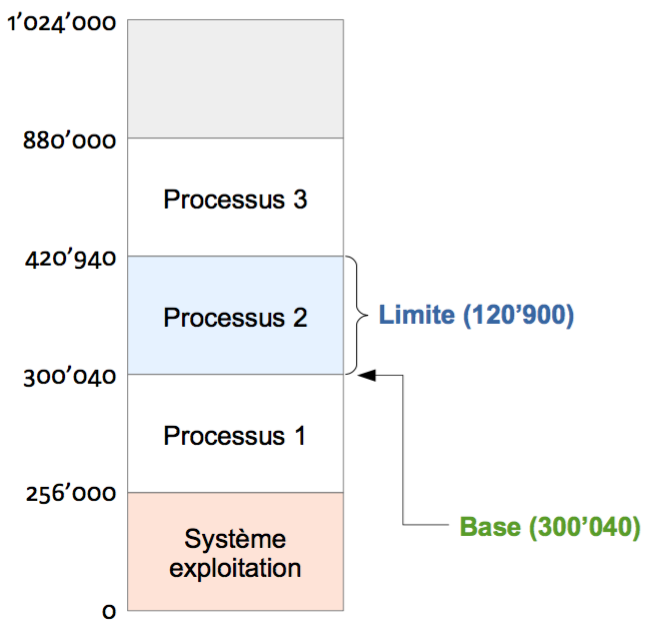
\includegraphics[scale=0.6]{images/ex_base_limit.png}
  \caption{Exemple d'adressage mémoire}
  \label{ex_base_limit}
\end{figure}

Une tache possède son propre espace d'adressage dit virtuel. Pour le processus 2
de la figure \ref{ex_base_limit}, l'adresse $0$ est en fait à l'adresse physique
$300040$. Il y a donc besoin de translater l'adresse virtuelle en adresse physique.
C'est là qu'entre en jeu le \acrshort{mmu} (Memory Mangement Unit). Le \acrshort{mmu}
est un dispositif matériel permettant de faire cette translation d'adresses. A chaque
référencement mémoire, il va convertir l'adresse virtuelle en adresse physique et
regarder si elle ne dépasse pas la limite du processus. Le \acrshort{mmu} permet donc
aussi de protéger la mémoire car il va empêcher toute référence à une zone extérieure
au processus (voir figure \ref{mmu}) \cite{ref42}.

\begin{figure}[!h]
  \centering
  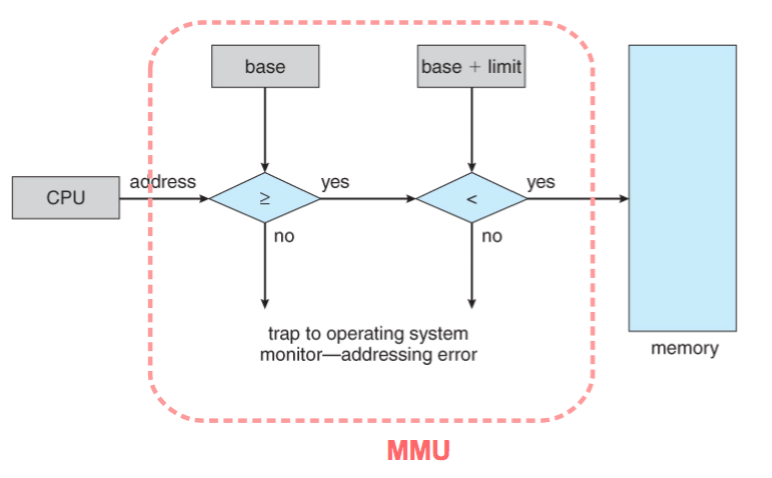
\includegraphics[scale=0.4]{images/mmu.png}
  \caption{Protection mémoire avec un \acrshort{mmu}}
  \label{mmu}
\end{figure}

Pour convertir une adresse virtuelle en adresse physique, le \acrshort{mmu} passe
par plusieurs étapes. Quand le \textit{kernel} veut lire une donnée dans la mémoire,
l'adresse de cette donnée est appelée adresse logique. Le \acrshort{mmu} va commencer
par convertir cette adresse en adresse linéaire. Une deuxième conversion est ensuite
effectuée afin d'obtenir une adresse physique. Le \acrshort{mmu} peut alors renvoyer
la bonne donnée au \textit{kernel}. Toutes ces étapes ne sont pas automatiques,
le \acrshort{mmu} utilise différentes techniques ayant besoin de certaines structures
implémentées par le \textit{kernel}. Ces techniques sont la segmentation et la
pagination.

\begin{figure}[!h]
  \centering
  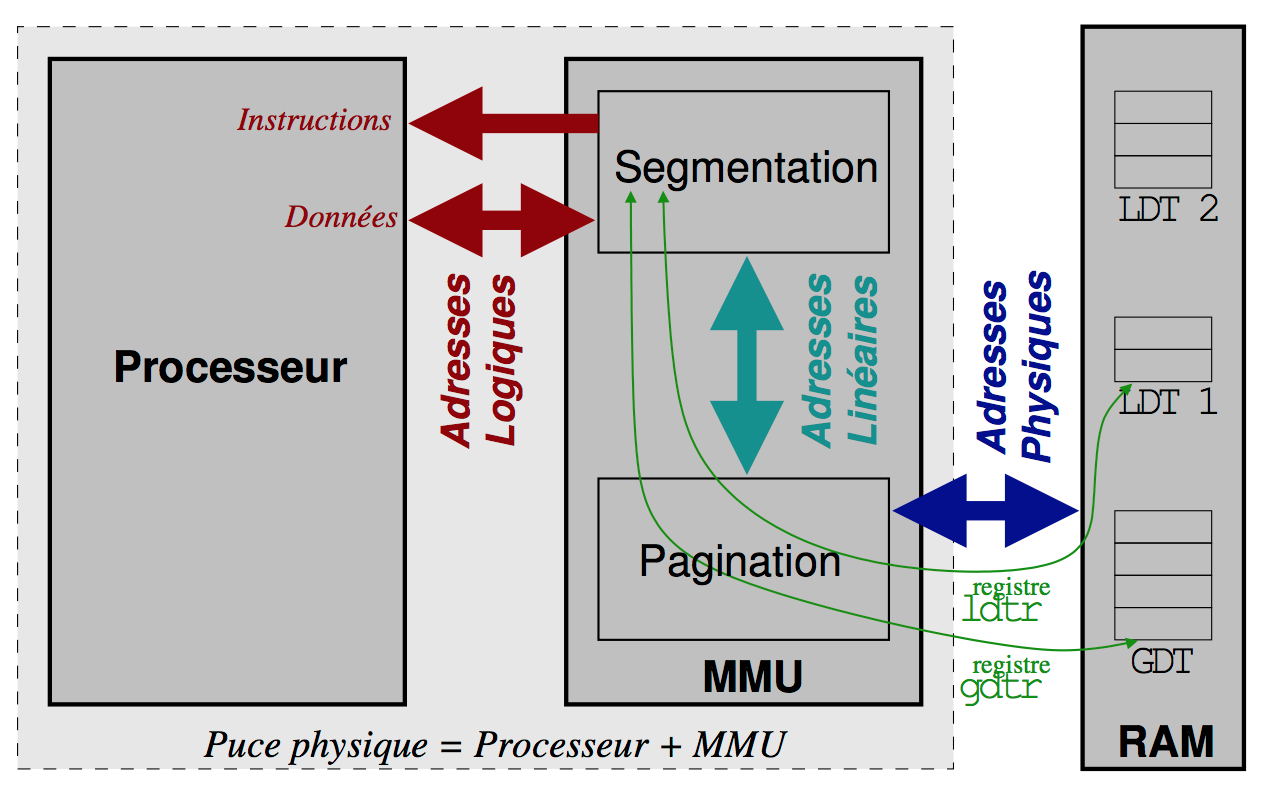
\includegraphics[scale=0.5]{images/addr_translation.png}
  \caption{Translation d'adresse}
  \label{addr_translation}
\end{figure}

La segmentation est une technique permettant de découper la mémoire en segments
de mémoire logique. Une adresse logique est convertie par le \acrshort{mmu} en
adresse linéaire en utilisant une table de descripteurs globale (\acrshort{gdt})
ou locale (\acrshort{ldt}). Si la pagination est activée, l'adresse linéaire est
convertie en adresse physique. Toute cette mécanique est décrite dans la figure
\ref{addr_translation}. A noter que la pagination n'est pas obligatoire et un
\acrshort{os} pourrait s'en passer contrairement à la segmentation qui est
indispensable en mode protégé (32-bits) \cite{ref17}.

%%%%%%%%%%%%%%%%%%%%%%%%%%%%%%%%%%%%%%%%%%%%%%%%%%%%%%%%%%%%%%%%%%
%%%%%%%%%%%%%%%%%%%%%%%%%%%%%%%%%%%%%%%%%%%%%%%%%%%%%%%%%%%%%%%%%%

\subsection{Segmentation}
\subsubsection{Principe général}
Comme expliqué précedemment, la segmentation est un mécanisme divisant l'espace
d'adressage du processeur en espaces d'adressage plus petits appelés des
segments. Un segment peut être utilisé pour contenir le code, les données ou la
pile d'un processus étant exécuté par le processeur. Un segment peut aussi être
utilisé pour contenir des structures de données tel qu'une \acrshort{ldt} ou
un \acrshort{tss} (structure contenant des informations à propos d'une tâche).
Les segments d'un système d'exploitation sont contenus dans l'espace d'adressage
linéaire. Pour lire l'octet d'un segment se trouvant dans l'espace d'adressage
linéaire, le \acrshort{mmu} utilise une adresse logique. L'adresse logique est
composée d'un sélecteur de segment et d'un \textit{offset}. Le sélecteur permet
de trouver le bon segment dans la mémoire linéaire et l'\textit{offset} permet
de trouver l'octet dans ce segment. Dans le cas où la segmentation est utilisée
seule (sans pagination), la mémoire linéaire est \textit{mappée} directement dans
la mémoire physique \cite{ref66}. \\

\begin{figure}[!h]
  \centering
  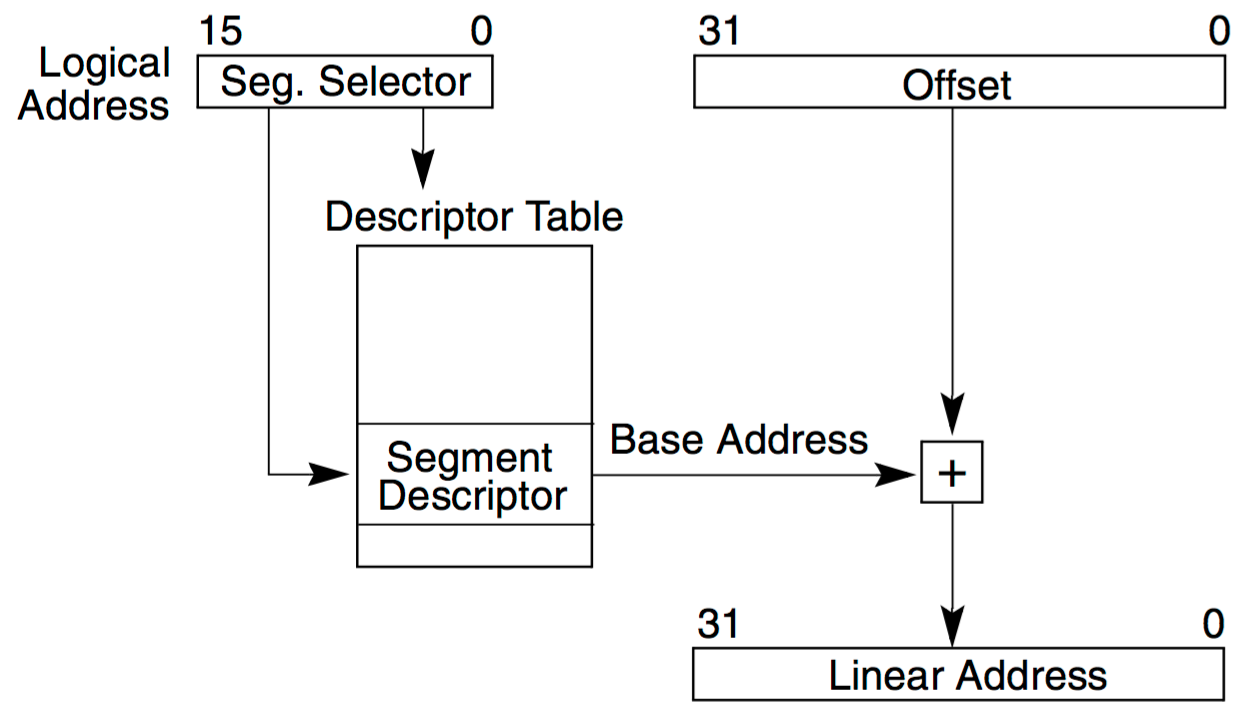
\includegraphics[scale=0.45]{images/logic_addr_conv.png}
  \caption{Conversion d'une adresse logique en adresse linéaire}
  \label{logic_addr_conv}
\end{figure}

La figure \ref{logic_addr_conv} résume bien la conversion d'adresse logique en
en adresse linéaire. On peut remarquer de plus que le sélecteur de segment passe
par une table de descripteurs (\acrshort{gdt} ou \acrshort{ldt}) afin de trouver
le bon segment dans la mémoire linéaire. En effet, Un sélecteur a une taille de
16 bits et contient l'index d'un descripteur dans une table, un bit indiquant si
le descripteur est dans la \acrshort{gdt} ou dans une \acrshort{ldt} et enfin son
niveau de privilège allant de 0 à 3 (figure \ref{seg_sel}) \cite{ref42}.

\begin{figure}[!h]
  \centering
  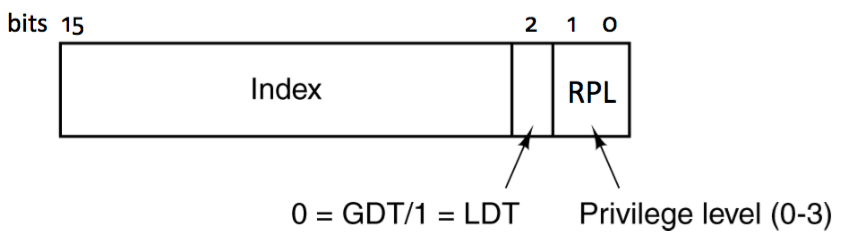
\includegraphics[scale=0.6]{images/seg_sel.png}
  \caption{Structure d'un sélecteur de segment}
  \label{seg_sel}
\end{figure}

La gestion de la segmentation par le \acrshort{cpu} se fait à l'aide de registres
spéciaux nommés registres de segment. Ces registres sont au nombre de six et ont
chacun une taille de 16 bits (même taille qu'un sélecteur de segment) \cite{ref42,ref18}.

\begin{center}
	\scalebox{.8}{
		\begin{tabular}{| C{5cm} | C{5cm} | }
			\hline
			Registre & Segment \\ \hline
			CS & \textit{Code Segment} \\ \hline
			DS & \textit{Data Segment} \\ \hline
			SS & \textit{Stack Segment} \\ \hline
			ES & \textit{Extra Segment} \\ \hline
			FS & \multirow{2}{*}{\textit{General Purpose Segments}} \\
            GS & \\ \hline
		\end{tabular}
	}
\end{center}

En mode protégé (32-bits), ces registres doivent pointer sur des descripteurs
de segment de la \acrshort{gdt}. Au minimum les trois premiers registres décrits
doivent être utilisé en mode protégé (CS, DS, et SS). Les opérations adressant
le code (décodage des instructons en mémoire, sauts, etc...) référencent le descripteur
de segment sur lequel pointe le registre CS. Les opérations adressant les données
(adressage de variables ou d'adresses mémoires) référencent le descripteur de segment
sur lequel pointe le registre DS. Les opérations adressant la pile (\mintinline{text}{push}
et \mintinline{text}{pop}) référencent le descripteur de segment sur lequel pointe
le registre SS. Ces registres pointent sur des descripteurs de segments par l'intermédiaire
de sélecteurs de segment. \\

\subsubsection{\acrshort{gdt} et \acrshort{ldt}}
\label{gdt_ldt}
Nous avons pu voir que pour translater une adresse logique, des sélecteurs de
segment sont utilisés. Ces sélecteurs pointent sur des entrées dans des tables
de descripteurs. La \acrshort{gdt} et la \acrshort{ldt} sont deux types de table 
de descripteurs différents. La \acrshort{gdt} est unique il ne peut y en avoir
qu'une seule dans le système. Elle contient toutes les données utilisables en mode
superviseur (\textit{ring} 0 ou niveau de privilège 0). Une \acrshort{ldt} est
contenue dans la \acrshort{gdt}. Elle peut être utilisée pour contenir le code
et les données d'une tâche utilisateur par exemple. Dans le cas où plusieurs tâches
sont exécutées en même temps, une \acrshort{ldt} peut être créée par tâche ce qui
permet en plus d'isoler le code de chaque processus. Une table de descipteurs
est composée, comme son nom l'indique, de descripteurs. Chaque descripteur décrit
une zone mémoire qui est défini par sa base (son adresse physique), sa limite (sa taille)
et un niveau de privilèges (allant de 0 à 3, le niveau 0 ayant le plus de privilèges
et le niveau 3 le moins). Ci dessous, la figure \ref{gdt} montre un exemple d'une
\acrshort{gdt} \cite{ref42}. Etant donné que les descripteurs de la \acrshort{gdt}
ont la même structure que les descripteurs de la \acrshort{ldt} nous allons nous
concentrer sur la \acrshort{gdt}. De plus, aucune \acrshort{ldt} n'est utilisé dans
la version actuelle de l'\acrshort{os}. \\

\begin{figure}[!h]
  \centering
  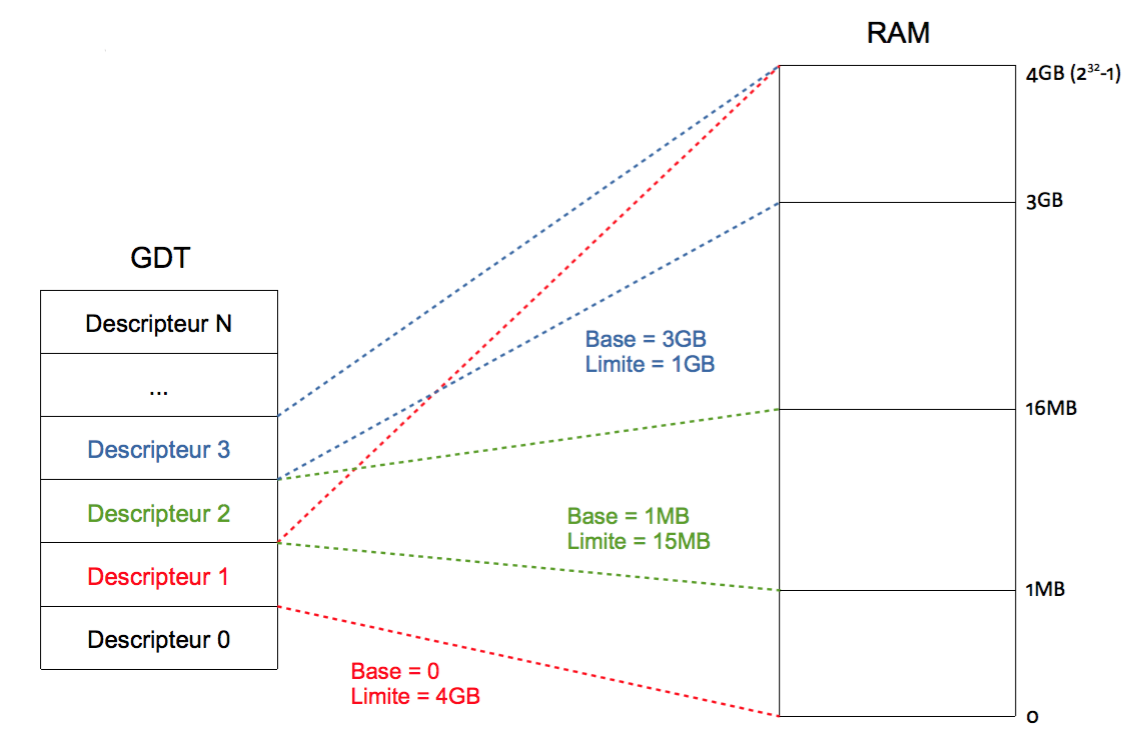
\includegraphics[scale=0.75]{images/gdt.png}
  \caption{Exemple d'une \acrshort{gdt}}
  \label{gdt}
\end{figure}

La \acrshort{gdt} est contenue en mémoire. Cette dernière doit être initialisée
par le \textit{kernel} avant d'être chargée et utilisée par le \acrshort{mmu}.
Pour initialiser la \acrshort{gdt} il faut construire ses entrées. Chaque entrée
(ou descripteur) de la table de descripteurs est sur 64 bit et décrit une zone
mémoire. L'adresse de cette zone mémoire est sur 32 bits et sa taille est sur 20
bits. Les bits restant sont des bits de contrôle pour l'accès aux données par
exemple (niveau de privilèfes, droit d'écriture/lecture, ...). Voir la figure
\ref{gdt_entry} pour plus de détails \cite{ref42,ref14}. \\

\begin{figure}[!h]
  \centering
  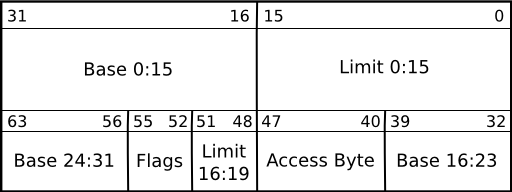
\includegraphics[scale=0.75]{images/gdt_entry.png}
  \caption{Structure d'une entrée dans la \acrshort{gdt}}
  \label{gdt_entry}
\end{figure}

L'\acrshort{os} développé a un adressage segmenté de type \textit{flat}, c'est-à-dire
que toute la mémoire est accédée de manière linéaire. Ce modèle de segmentation
est le plus simple car il permet d'ignorer le mécanisme de segmentation car
l'intégralité de la zone mémoire devient disponible. Dans un modèle de type \textit{flat},
les segments de code et de données se chevauchent sur l'intégralité de la mémoire
disponible. Ceci se fait en initialisant trois descripteurs dans la \acrshort{gdt}.
Un descripteur nul à l'index 0 (obligatoire dans touts les modèles de segmentation),
un segment de code couvrant toute la mémoire et un segment de données couvrant
aussi toute la mémoire. Les segments de code et de données adressent ainsi les mêmes
zones mémoire. On verra par la suite que d'autres entrées ont été aujoutées à la
\acrshort{gdt} pour la gestion des tâches. \\

\begin{figure}[!h]
  \centering
  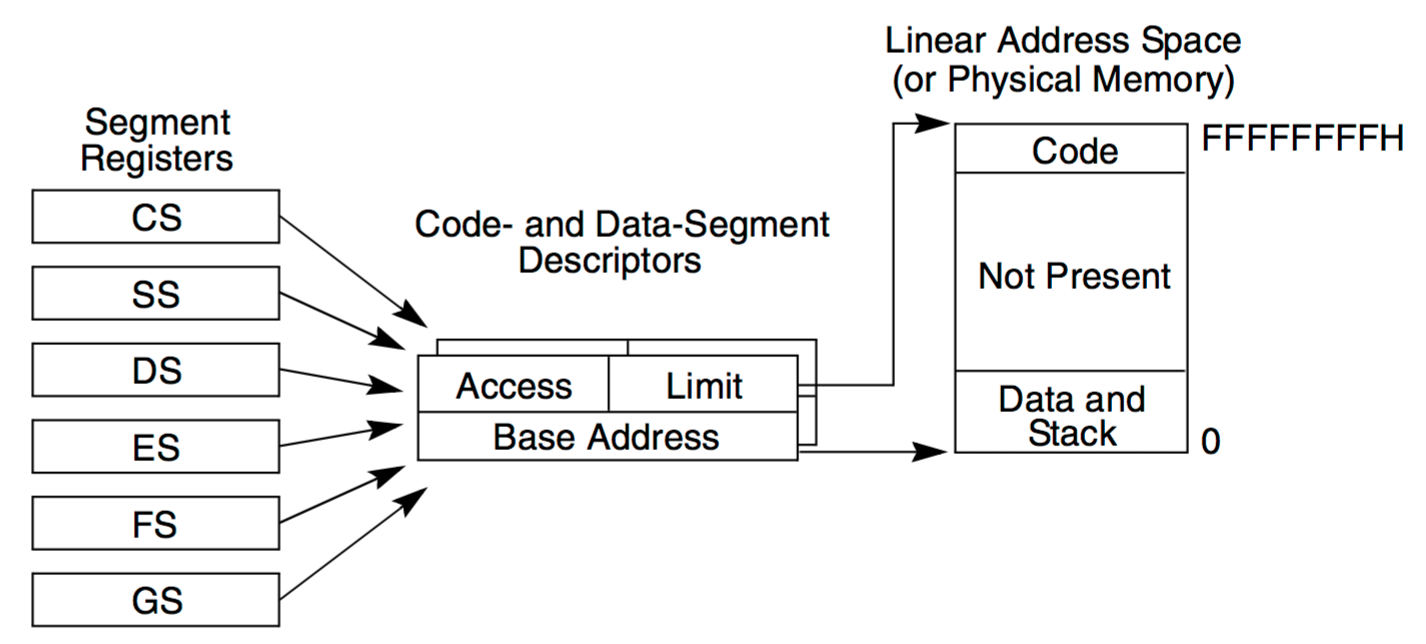
\includegraphics[scale=0.6]{images/flat.png}
  \caption{Modèle de segmentation de type \textit{flat}}
  \label{flat}
\end{figure}

Pour obtenir un  segment sur toute la mémoire disponible, il faut mettre le bit
de granularité à 1 pour avoir une limite en blocs de 4Ko. Ensuite, la limite doit
être mise à la valeur 0xFFFFF ce qui donne une limite réele de 0x100000 $\times$
0x1000 soit 4Go. Le niveau de privilège doit être laissé à 0 (\textit{ring} 0)
si on veut créer un segment pour le \textit{kernel} ou bien être mis à 3 (\textit{ring}
3) si on veut créer un segment pour le mode utilisateur. Ci-dessous un exemple de
code permettant de construire un segment de code et un segment de données. \\

\begin{minted}[fontsize=\footnotesize,tabsize=4,frame=single]{rust}
fn new(base: u32, limit: u32, type: u8, s: u8, d: u8, g: u8, dpl: u8) -> GdtEntry;

pub fn make_code_segment(base: u32, limit: u32, dpl: u8) -> GdtEntry {
    GdtEntry::new(base, limit, 0xB, 0x1, 0x1, 0x1, dpl)
}

pub fn make_data_segment(base: u32, limit: u32, dpl: u8) -> GdtEntry {
    GdtEntry::new(base, limit, 0x3, 0x1, 0x1, 0x1, dpl)
}
\end{minted}

Ici, \mintinline{rust}{new} est le prototype d'une méthode pour une structure 64
bits représentant une entrée dans la \acrshort{gdt}. le bit \mintinline{rust}{s}
est mis à 1 car on construit des segments de code et de données \cite{ref66}.
Le bit \mintinline{rust}{d} est mis à 1 car on veut un segment de 32 bits. Le bit
\mintinline{rust}{g} est mis à 1 pour avoir une granularité de 4Ko. L'octet 0xB
correspond au type $CODE\_EXEC\_READ$ et 0x3 correspond au type $DATA\_READ\_WRITE$
\cite{ref42}. Une fois la \acrshort{gdt} construite, il faut dans un premier temps
utiliser l'instruction \mintinline{text}{lgdt} pour la charger dans le registre
GDTR. Ce registre est utilisé par le processeur pour faire le lien entre le \acrshort{mmu}
et la \acrshort{gdt} créée \cite{ref66}. L'adresse du descripteur de la \acrshort{gdt}
doit donc être donnée en argument à l'instruction \mintinline{text}{lgdt}. Le
descripteur de \acrshort{gdt} est défini par la structure 48-bits décrite dans
la figure \ref{gdt_descriptor} \cite{ref14}.

\begin{figure}[!h]
  \centering
  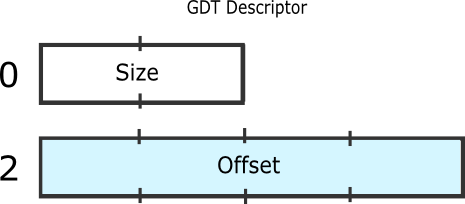
\includegraphics[scale=0.5]{images/gdt_descriptor.png}
  \caption{Descripteur de \acrshort{gdt}}
  \label{gdt_descriptor}
\end{figure}

Dans un descripteur de \acrshort{gdt} \textit{Size} est la limite sur 16 bits
(c'est à dire la taille de la \acrshort{gdt} - 1) et \textit{Offset} est l'adresse
physique de la \acrshort{gdt} sur 32 bits. Dans le cas de notre \acrshort{os},
la \acrshort{gdt} est déclarée statiquement dans le \textit{kernel}. L'adresse
de cette variable statique est utilisée pour construire un descripteur qui sera
chargé dans le registre GTDR. Après avoir chargé la \acrshort{gdt} avec l'instruction
\mintinline{text}{lgdt}, il faut faire pointer les registres de segment sur les
segments de la table de descripteurs à l'aide de sélecteurs. Pour rappel, un sélecteur
est sur 16 bits et contient l'index d'un segment dans la \acrshort{gdt} précedemment
chargée. Pour récupérer l'index d'un segment dans la \acrshort{gdt} à partir de
l'index de son descripteur, il faut faire un décallage à gauche de 3 bits
(voir figure \ref{seg_sel}). Prennons un descripteur se situant à l'index 2 de
la \acrshort{gdt}. Si on veut initialiser le segment de code (registre CS) avec
ce descripteur, il faut mettre la valeur 16 dans le registre CS ($2 << 3 = 16$).
Dans le cas où on veut définir ce segment avec un autre niveau de privilèges
ou bien pour une \acrshort{ldt}, il suffit de mettre les bons bits à 1 après avoir
fait le décallage.

\newpage
%%%%%%%%%%%%%%%%%%%%%%%%%%%%%%%%%%%%%%%%%%%%%%%%%%%%%%%%%%%%%%%%%%
%%%%%%%%%%%%%%%%%%%%%%%%%%%%%%%%%%%%%%%%%%%%%%%%%%%%%%%%%%%%%%%%%%

\subsection{Pagination}
\subsubsection{Principe général}
La pagination est une autres technique de gestion de mémoire qui diffère de la
segmentation. Alors que la segmentation permet d'allouer des morceaux de mémoire
de taille variable, la pagination divise la mémoire en blocs de taille fixe appelés
pages (de 4Ko, 2Mo ou 4Mo). De plus, la segmentation est obligatoire dans une
architecture i386 alors que la pagination ne l'est pas \cite{ref16}. Quand une tâche
fait référence à une adresse logique en mémoire, cette adresse est convertie en
adresse linéaire grace au mécanisme de segmentation et c'est le mécanisme de
pagination qui permet de translater cette adresse linéaire en adresse physique
(comme vu précedemment dans la partie sur la segmentation). Quand la
pagination est activée, l'adresse linéaire est divisée en deux parties lorsque
des pages de 4Mo sont utilisées et en trois parties lorsque des pages de 4Ko
sont utilisées. Le \textit{kernel} développé utilise des pages de 4Ko, une adresse
linéaire est donc sous la forme suivante :

\begin{itemize}[label=\textbullet]
	\item 10 bits pour le \textit{directory index}
	\item 10 bits pour le \textit{page index}
    \item 12 bits pour l'\textit{offset}
\end{itemize}

On dit que cette pagination est une pagination à trois niveaux. En général, une
pagination à trois niveaux est utilisée mais il peut exister des systèmes utilisant
plus ou moins de niveaux. Le système d'exploitation doit créer un répertoire de pages
(\textit{Page Directory}) et au moins une table des pages (\textit{Page Table}) pour
chaque tâche. Les répertoires et les tables des pages ont la taille d'une page et sont
composés d'entrées sur 32 bits (4 octets). Une entrée dans un répertoire permet
d'adresser une table de pages et une entrée dans une table permet d'adresser une page.
Dans notre cas, un répertoire permet donc d'adresser 1024 tables et une table
1024 pages ce qui permet bien d'adresser au total 4Go ($1024 \times 1024 \times 4096$).
Une entrée est sur 32 bits mais seulement les 20 bits de poids fort sont utilisés
pour l'adressage car les adresses sont alignées avec 4096 ce qui laisse les 12 bits
de poids faible pour la configuration \cite{ref21}.

\begin{figure}[!h]
  \centering
  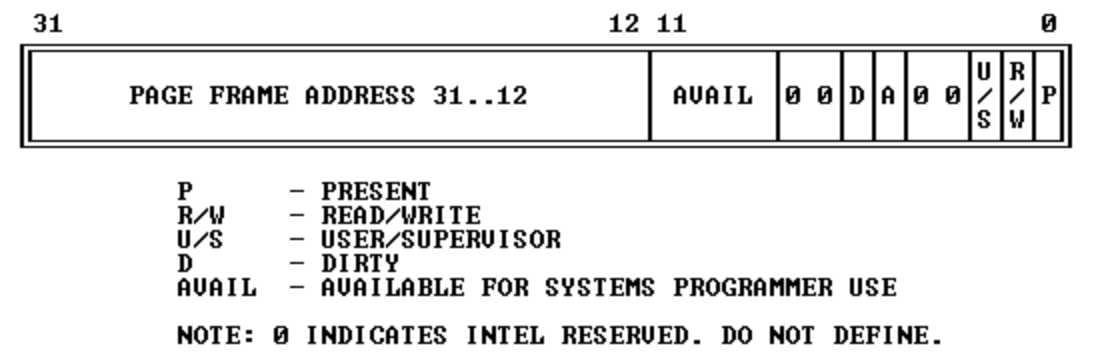
\includegraphics[scale=0.6]{images/page_entry.png}
  \caption{Structure d'une \textit{Page Entry}}
  \label{page_entry}
\end{figure}

Quand une adresse linéaire est lue, le \textit{directory index} permet
de lire la bonne entrée dans le \textit{Page Directory}. Il faut ensuite utiliser
le \textit{page index} pour récupérer la bonne entrée dans la table des pages.
De la même manière que l'entrée dans le répertoire de pages pointait sur une table
des pages, l'entrée dans une table des pages pointe sur une \textit{Page Frame}.
Cette page contient finalement la donnée pointée par l'adresse linéaire, il faut
utiliser l'\textit{offset} pour trouver cette donnée dans la page. La figure \ref{paging3}
résume bien ce mécanisme \cite{ref66}. A noter que le \textit{Page Directory} est
pointé par le registre CR3. A chaque fois qu'un changement de tâche a lieu, le
registre CR3 doit être mis à jour avec le \textit{Page Directory} de la nouvelle
tâche \cite{ref15}.

\begin{figure}[!h]
  \centering
  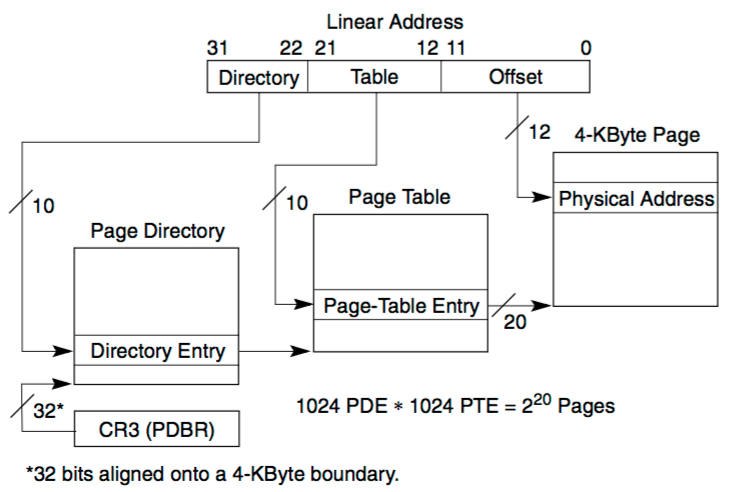
\includegraphics[scale=0.85]{images/paging3.png}
  \caption{Exemple de pagination à 3 niveaux}
  \label{paging3}
\end{figure}

%%%%%%%%%%%%%%%%%%%%%%%%%%%%%%%%%%%%%%%%%%%%%%%%%%%%%%%%%%%%%%%%%%

\subsubsection{Activation de la pagination}
\label{activate_paging}
Pour initialiser la pagination sur architecture x86, il faut d'abord construire
un répertoire de pages valide contenant les entrées vers les pages du \textit{kernel}.
Il est obligatoire de commencer par cela car si la pagination est activée et que
le \textit{kernel} n'est pas \textit{mappé} dans le répertoire chargé, une exception
sera levée (\textit{Page Fault}). Par soucis de simplicité pour la suite du développement
de l'\acrshort{os}, le \textit{kernel} va être déplacé au dernier Go de la \acrshort{ram}.
Grace à la pagination, ceci peut se faire assez simplement, il suffit de compléter
le répertoire de pages ainsi que ses tables de pages correctement. Pour rappel,
le \textit{kernel} commence à l'adresse 0x100000 (1Mo) mais il faut aussi rendre
accessible le premier Mo de \acrshort{ram}. Il faut donc déplacer les adresses physiques
allant de 0x0 à la fin du kernel (qui n'est pas fixe). Dans un premier temps, le
\textit{linker} doit être modifié de cette manière :

\begin{minted}[fontsize=\footnotesize,linenos,frame=single,tabsize=4]{c}
SECTIONS {
    /* Low memory Kernel */
    . = 0x00100000;
    .boot ALIGN(4) :        { *(.multiboot) }
    .low_text ALIGN (4K) :  { *(.low_text) }
    .low_data ALIGN (4K) :  { *(.low_data) }
    .low_bss ALIGN (4K) :   { *(.low_bss) }
    /* Higher-half Kernel */
    . += 0xC0000000;
    .stack ALIGN(4) : AT(ADDR(.stack) - 0xC0000000)     { *(.stack) }
    .text ALIGN(4K) : AT(ADDR(.text) - 0xC0000000)      { *(.text*) }
    .rodata ALIGN(4K) : AT(ADDR(.rodata) - 0xC0000000)  { *(.rodata*) }
    .data ALIGN(4K) : AT(ADDR(.data) - 0xC0000000)      { *(.data*) }
    .bss ALIGN(4K) : AT(ADDR(.bss) - 0xC0000000)        { *(COMMON) *(.bss*) }
}
\end{minted}

Ici, le \textit{kernel} est divisé en deux parties. La première est celle qui va
être appelée au démarrage du système et qui va initialiser la pagination. Une fois
la pagination active, le \textit{kernel} va continuer son exécution dans la deuxième
partie qui est située dans le dernier Go de \acrshort{ram}. Nous sommes obligés de
démarrer le \textit{kernel} au début de la mémoire physique car toutes les adresses
sont virtuelles. En réalité, le \textit{kernel} dispose de beaucoup moins (variable
selon la configuration de l'émulateur, ici QEMU). Il n'existe donc pas d'adresse
physique située à 3Go dans la mémoire physique du \textit{kernel} et il est donc
impossible de démarrer le système à cette adresse. Regardons plus en détail de quelle
manière la première partie du \textit{kernel} initialise la pagination. Comme dit
précedemment, un répertoire de pages initial doit être construit. Etant donné que
nous allons exécuter du code dans le premier Go et aussi dans le dernier, le \textit{kernel}
doit être \textit{mappé} dans ces deux zones mémoire en même temps. La première
partie va être adressée linéairement, ce qui veut dire que l'adresse physique
0x0 correspondra à l'adresse virtuelle 0x0 et ainsi de suite jusqu'à la fin du
\textit{kernel}. Cet adressage donne le répertoire de pages shématisé dans la figure
\ref{low_kern_pd}.

\begin{figure}[!h]
  \centering
  \includegraphics[scale=0.65]{images/low_kern_pd.png}
  \caption{Répertoire de pages adressant le \textit{kernel} au début de la \acrshort{ram}}
  \label{low_kern_pd}
\end{figure}

On peut voir ici que la première entrée du répertoire de pages pointe sur une
table de pages adressant le début de la \acrshort{ram}. Chaque entrée est incrémentée
de 4096 (0x1000 en hexadécimal) car une page fait 4096 octets. De plus, les deux
premiers bits de poids faible de chaque page sont à 1 pour indiquer que la page est
active et que l'on peut écrire et lire dedans (voir figure \ref{page_entry}). L'entrée
dans le répertoire de page correspondant au dernier Go (soit 0xC0000000 en hexadécimal)
doit pointer sur une table des pages identique. Pour trouver une entrée dans le
répertoire de pages depuis une adresse il faut faire un décallage à droite de 22
bits sur cette adresse (ce qui est équivalent à diviser par 4096, soit la taille
d'une page, puis de nouveau diviser par 1024, soit le nombre de pages adressées par
une table). Ici, 0xC0000000 $>>$ 22 = 0x300 (768 en décimal). Il faut donc faire
pointer l'entrée 768 du répertoire de pages à une table des pages identique à
celle pointée par l'entrée 0 ce qui donne finalement le répertoire suivant.

\begin{figure}[!h]
  \centering
  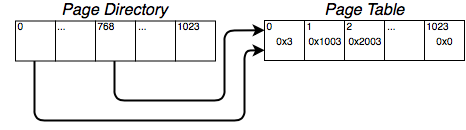
\includegraphics[scale=0.65]{images/high_kern_pd.png}
  \caption{Répertoire de pages adressant le \textit{kernel} à la fin de la \acrshort{ram}}
  \label{high_kern_pd}
\end{figure}

Une fois le répertoire de pages initialisé de cette manière, il ne reste plus
qu'à faire pointer le registre CR3 dessus et activer la pagination en mettant
le bit 31 du registre CR0 à 1. Le code peut ensuite sauter à la partie haute de
la \acrshort{ram} où nous avons déplacé le \textit{kernel}. A partir de là,
tout le code qui sera exécuté sera dans le dernier Go de \acrshort{ram}, il n'y
a donc plus besoin de faire pointer la première entrée du répertoire de pages
sur le table des pages du \textit{kernel} ce qui peut être fait en écrivant 0
dans cette entrée. Le code rust peut finalement être appelé avec la pagination
active.

%%%%%%%%%%%%%%%%%%%%%%%%%%%%%%%%%%%%%%%%%%%%%%%%%%%%%%%%%%%%%%%%%%

\subsection{Allocation dynamique en mode \textit{kernel}}
Le dernier élément de gestion mémoire implémenté dans RustOS est l'allocation de
mémoire dynamique. L'allocation dynamique consiste à réserver des blocs de mémoire
pendant l'exécution du \textit{kernel} ou bien d'un programme utilisateur. Jusqu'à
maintenant, toutes les structures utilisées était déclarées statiquement se retrouvant
donc dans la zone mémoire du \textit{kernel}, plus précisément dans le segment
bss (voir \ref{linking}). Déclarer des variables statiquement est pratique mais fait
augmenter la taille du \textit{kernel} et ce n'est pas une solution viable
pour allouer de plus grandes régions mémoire comme par exemple du code utilisateur
qui peut faire plusieurs kilooctets. Pour implémenter l'allocation de mémoire
dynamique, il faut dans un premier temps définir quelle zone mémoire peut être
utilisée dans ce but. Actuellement, la totalité du code et des données est contenu
dans le \textit{kernel}. Des zone mémoire peuvent donc commencer à être allouées
à la fin de ce dernier. Le \textit{linker} a été légèrement modifié afin d'obtenir
l'adresse de la fin du \textit{kernel}. Ceci peut se faire en ajoutant une expression
au \textit{linker} et en la rendant accessible depuis le code assembleur. \\

Modification apportée au \textit{linker} :
\begin{minted}[fontsize=\footnotesize,linenos,frame=single,tabsize=4]{c}
. += 0xC0000000;
...
kernel_end = .;
\end{minted}

Code assembleur permettant de rendre accessible l'expression \mintinline{c}{kernel_end} :
\begin{minted}[fontsize=\footnotesize,linenos,frame=single,tabsize=4]{text}
extern kernel_end
get_kernel_end:
    mov eax, kernel_end
    ret
\end{minted}

A partir de là, on peut définir la zone d'allocation mémoire aussi appelée tas
(ou \textit{heap} en anglais). Dans notre \acrshort{os}, le tas commence à la
fin du \textit{kernel} allignée avec la taille d'une page (4096 octets). Ce choix
a été fait car le \textit{kernel} n'aura besoin d'allouer que des nouvelles
pages. La fin du tas dépend de la fin de la mémoire physique qui dépend de la
configuration de QEMU. Quand le \textit{kernel} aura besoin d'allouer une nouvelle
page, il ira chercher le prochain bloc libre dans le tas situé donc entre la fin
du \textit{kernel} et la fin de la mémoire physique. La recherche de bloc libre
se complexifie rapidement si des blocs sont libérés. De nombreuses méthodes sont
possibles pour la recherche de bloc libre et la gestion des blocs libérés. Le
\textit{kernel} développé utilisé une liste doublement chaînée pour gérer la
mémoire dynamique. Chaque bloc mémoire alloué est précédé d'un entête contenant
l'adresse du bloc précédent sur 32 bits, l'adresse du bloc suivant sur 32 bits,
sa taille en octets sur 32 bits et un booléen indiquant si le bloc est libre ou
non sur 8 bits. De plus, l'entête est aligné sur 16 octets.

\begin{figure}[!h]
  \centering
  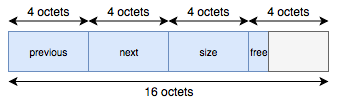
\includegraphics[scale=0.7]{images/heap_header.png}
  \caption{Entête d'un bloc de mémoire dans le tas}
  \label{heap_header}
\end{figure}

Le tas ainsi construit, avec chaque entête lié à ses voisins par des pointeurs,
permet de rechercher aisément un bloc libre. Un nouvel entête est créé quand le
dernier bloc de la liste chaînée est alloué. Un algorithme a aussi été implémenter
pour la gestion de mémoire libérée. Si un bloc est libéré au milieu de blocs
alloués ce blocs est simplement marqué comme libre (en utilisant le booléen \textit{free}
de l'entête). Si deux blocs libres sont contiguës, ils sont fusionnés pour n'en
former qu'un seul. Dans le \textit{kernel}, la fonction pour l'allocation est
\mintinline{rust}{kmalloc} et la fonction pour la libération est \mintinline{rust}{kfree}.
La fonction \mintinline{rust}{kmalloc} va allouer de nouvelles pages et tables
de pages automatiquement s'il y a besoin (comme le montre la figure \ref{kmalloc}).
De la même manière, la fonction \mintinline{rust}{kfree} va libérer les pages et
les tables de pages automatiquement. Ces deux fonctions permettent donc beaucoup
d'abstraction au niveau de la pagination mais aussi de l'allocation car l'utilisation
des entêtes est complètement transparent. La fonction \mintinline{rust}{kmalloc}
va simplement renvoyer une adresse sur 32 bits et \mintinline{rust}{kfree} prend
comme argument cette adresse pour libérer la mémoire.

\begin{figure}[!h]
  \centering
  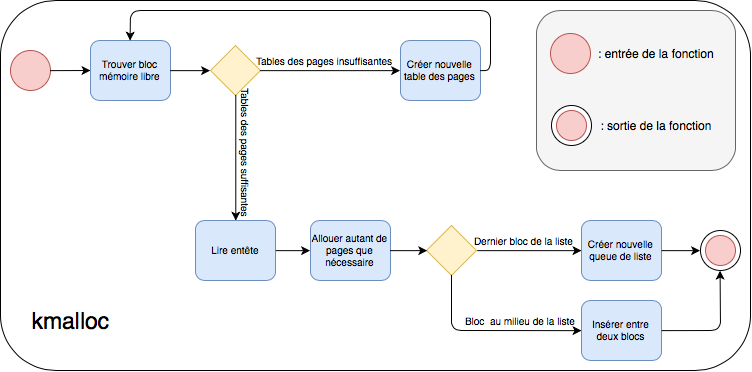
\includegraphics[scale=0.6]{images/kmalloc.png}
  \caption{Algorithme utilisé pour l'allocation dynamique dans le \textit{kernel}}
  \label{kmalloc}
\end{figure}

Voyons maintenant un exemple d'allocation et de libération mémoire utilisant les
deux algorithmes décrits ci-dessus. Dans cet exemple, nous allons allouer plusieurs
blocs mémoire puis les libérer afin de voir plus en détail le comportement
de ces fonctions. Nous allons supposé que la fin du \textit{kernel} se situe
à l'adresse 0x3FC000 et que la fin de la \acrshort{ram} se situe à l'adresse
0x1000000. A l'initialisation du \textit{kernel}, un premier entête est créé au
début de la zone d'allocation dynamique. Ce premier entête est donc situé à
l'adresse 0x3FC000 et a pour taille 0x1000000 $-$ 0x3FC000 $=$ 0xC04000. C'est cette
information qui permet de trouver la premier entrée de la liste et par la suite
de la parcourir.

\begin{figure}[!h]
  \centering
  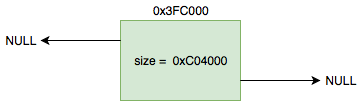
\includegraphics[scale=0.7]{images/alloc0.png}
  \caption{Etat initial de la chaîne d'entêtes}
  \label{alloc0}
\end{figure}

Si le \textit{kernel} a besoin d'allouer une nouvelle page maintenant, la fonction
\ref{kmalloc} va être appelée qui va parcourir les blocs libre. Dans ce cas précis,
l'intégralité du tas est disponible donc la fonction va simplement créer un nouveau
bloc. Dans la figure \ref{alloc1}, les blocs libre sont en vert et les blocs alloués
sont en rouge. A noter que que les blocs aloués sont alignés avec la taille d'une
page (4096Ko ou 0x1000 en hexadécimal). Etant donné qu'il faut compté l'entête
de 16 octets, il faudra toujours allouer une page de plus.

\begin{figure}[!h]
  \centering
  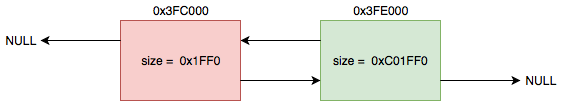
\includegraphics[scale=0.6]{images/alloc1.png}
  \caption{Allocation d'une page}
  \label{alloc1}
\end{figure}

Si le \textit{kernel} a de nouveau besoin d'une page, on va se retrouver dans la
situation où il n'y a plus assez de place dans la table des pages. Pour rappel,
une table des pages a une taille de 4Mo (0x400000 en hexadécimal). Comme expliqué
avec la figure \ref{kmalloc}, la fonction d'allocation va se charge toute seule
de créer une nouvelle table des pages et de l'ajouter au répertoire de pages.
La page demandée par le \textit{kernel} sera ensuite allouée. On obtient donc
la liste de la figure \ref{alloc2}, avec deux blocs alloués au lieu d'un seul.
Le bloc à l'adresse 0x3FE000 contient alors la table des pages sur laquelle pointe
la deuxième entrée du répertoire des pages. La page demandée par le \textit{kernel}
sera finalement à l'adresse 0x400000.

\begin{figure}[!h]
  \centering
  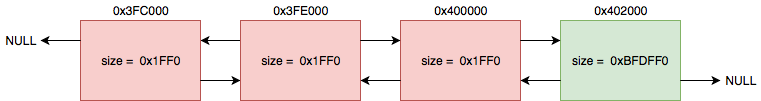
\includegraphics[scale=0.6]{images/alloc2.png}
  \caption{Allocation d'une page et d'une table des pages}
  \label{alloc2}
\end{figure}

Libérer la page à l'adresse 0x400000 aura pour conséquence directe de libérer aussi
la table des pages nouvellement créée (la fonction \mintinline{rust}{kfree} libère
automatiquement les tables des pages vides). On se retrouverait alors avec le même
schéma que dans la figure \ref{alloc1} car les blocs aux adresses 0x3FE000 et
0x400000 seraient fusionnés au reste de la mémoire libre.

%%%%%%%%%%%%%%%%%%%%%%%%%%%%%%%%%%%%%%%%%%%%%%%%%%%%%%%%%%%%%%%%%%
%%%%%%%%%%%%%%%%%%%%%%%%%%%%%%%%%%%%%%%%%%%%%%%%%%%%%%%%%%%%%%%%%%

\newpage
\section{Périphériques}
%%%%%%%%%%%%%%%%%%%%%%%%%%%%%%%%%%%%%%%%%%%%%%%%%%%%%%%%%%%%%%%%%%
%%%%%%%%%%%%%%%%%%%%%%%%%%%%%%%%%%%%%%%%%%%%%%%%%%%%%%%%%%%%%%%%%%

\subsection{Ports}
Un processeur \acrshort{IA-32} a la possibilité de transférer des données en utilisant
les ports d'entrée/sortie. Ces ports sont utilisés par le processeurs pour communiquer
avec des périphériques. Il peuvent être utilisés pour envoyer et recevoir des données
(par exemple un \textit{timer} va utiliser les ports d'entrée/sortie pour envoyer
son état). Les ports peuvent aussi être utilisés pour contrôler un péripéhrique
à partir de registres de contrôle (par exemple avec un controlleur de disque).\cite{ref64}
Etant donné que nous ne sommes pas sur du vrai \textit{hardware}, QEMU va se charger
d'émuler les différents périphériques utilisés par un processeur Intel 32-bits. \\

Les ports d'entrées/sorties sur architecture x86 se situent dans un espace d'adresses
séparé de la mémoire physique. Cet espace permet d'adresser 64000 (soit $2^{16}$)
ports de 8 bits. Les ports sont donc adressés sur 16 bits mais  il n'est pas possible
d'écrire dans un \acrshort{pio} de la même manière que l'on écrirait dans la mémoire
(avec une instruction  \mintinline{text}{MOV}) car nous sommes dans deux
espaces d'adresses différents. Ainsi, le \acrshort{cpu} utilise des instructions speciales
pour accéder aux \acrshort{pio}. Ces instructions sont les instructions
\mintinline{text}{IN} et \mintinline{text}{OUT}. \mintinline{text}{IN} permet de lire
tandis que \mintinline{text}{OUT} permet d'écrire. A noter que l'adresse du port
doit toujours être spécifiée dans le registre \mintinline{text}{dx} et la lecture
et l'écriture se font toujours avec les registres \mintinline{text}{ax/al}.\cite{ref42} \\

\begin{multicols}{2}
    [
    Exemple de lecture et d'écriture dans un port d'entrée/sortie :
    ]
    Ecrire 4 dans le port 0x2A :
    \begin{minted}[fontsize=\footnotesize,tabsize=4]{text}
        mov dx, 0x2A
        mov al, 4
        out dx, al
    \end{minted}
    \columnbreak
    Lire un octet depuis le port 0x2A :
    \begin{minted}[fontsize=\footnotesize,tabsize=4]{text}
        mov dx, 0x2A
        in  byte al, dx
    \end{minted}
\end{multicols}

Il existe une autre méthode pour écrire dans les ports utilisant le même bus d'adresse
pour la mémoire physique et pour les périphériques. Cette méthode consiste à
\textit{mapper} les ports d'entrées/sorties dans la mémoire physique (\acrshort{mmio}).
En écrivant dans la zone reservée aux ports, on écrirait alors directement dans
les ports et pas dans la mémoire physique. Le \textit{kernel} développé utilise
la première méthode (\acrshort{pio}).

%%%%%%%%%%%%%%%%%%%%%%%%%%%%%%%%%%%%%%%%%%%%%%%%%%%%%%%%%%%%%%%%%%
%%%%%%%%%%%%%%%%%%%%%%%%%%%%%%%%%%%%%%%%%%%%%%%%%%%%%%%%%%%%%%%%%%

\subsection{Interruptions et Exceptions}
\subsubsection{Principe général}
Les interruptions et les exceptions sont des évenements qui indiquent que l'attention
du processeur est demandée quelque part soit dans le code, soit par un périphérique.
Il existe deux types d'interruptions, les interruptions logicielles et les interruptions
matérielles. Les exceptions sont générées par le processeur mais diffèrent des
interruptions logicielles. Une interruption peut arriver à n'importe quel moment
en réponse au signal d'un périphérique ou bien si le processeur le demande
avec l'instruction \mintinline{text}{INT} (interruption logicielle). Une exception
est levée lorsque le processeur détecte une erreur à l'exécution d'une instruction
(par exemple une division par 0). Quand une interruption ou une exception
a lieu, une routine logicielle est appelée (\acrshort{isr}). Les processeurs \acrshort{IA-32}
supportent jusqu'à 256 interruptions dont les 32 premières sont reservées aux exceptions
processeur (voir figure \ref{table_int_exc}).\cite{ref42,ref66} \\

\begin{figure}[!h]
  \centering
  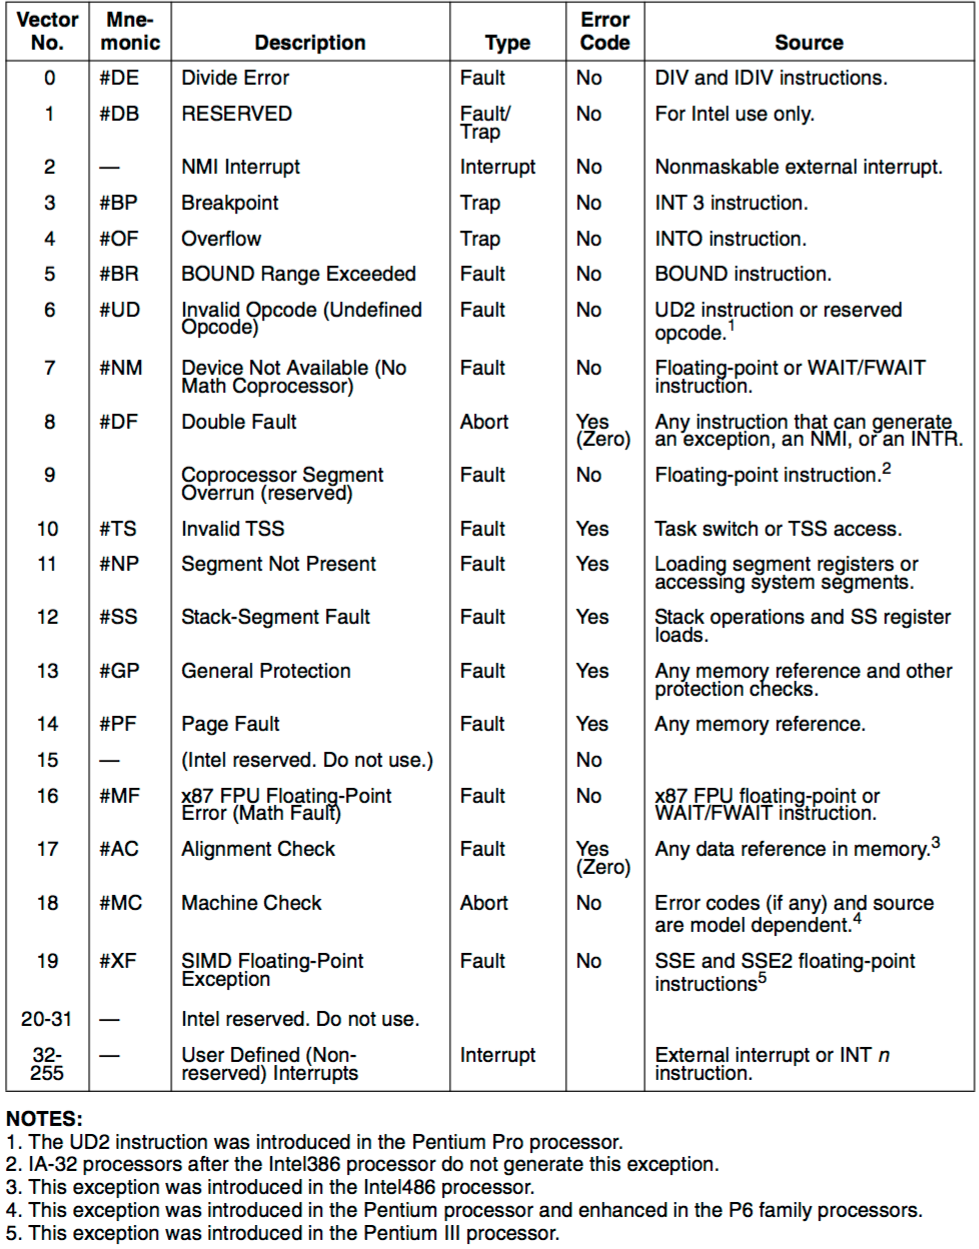
\includegraphics[scale=0.39]{images/table_int_exc.png}
  \caption{Table des interruptions et exceptions sur \acrshort{IA-32}}
  \label{table_int_exc}
\end{figure}

Comme vu précedemment, une interruption logicielle peut être exécutée par le
processeur avec l'instruction \mintinline{text}{INT}. L'instruction \mintinline{text}{INT}
suivie du numéro d'interruption sur 8 bits déclenchera l'interruption en question.
Par exemple, l'instruction \mintinline{text}{INT 0x30} déclenchera l'interruption
48. Au moment de l'appel à l'instruction \mintinline{text}{INT}, le pointeur
d'instruction va sauter à l'adresse du code contennant la routine d'interruption
correspondant au numéro d'interruption logicielle specifiée. C'est la table des
descripteurs d'interruption (\acrshort{idt}) qui permet de définir l'adresse du
code à exécuter pour chaque numéro d'interruption (que ce soit une interruption
logicielle, matérielle ou une exception). A noter aussi que les interruptions
logicielles sont synchrone étant donné qu'elles sont exécutées par le processeur,
contrairement aux interruptions matérielles qui sont asynchrones (exécutées par
les périphériques, elle peuvent arriver à n'importe quel moment). \\

Nous avons vu que les interruptions matérielles étaient générées par le \textit{hardware}.
Il existe deux types d'interruptions matérielles, les \acrshort{nmi} (\textit{Non Maskable
Interrupt}) et les \acrshort{irq} (Interrupt Request). Une \acrshort{nmi} indique
qu'un problème est survenu au niveau matériel (mémoire défectueuse, erreur de bus, ...).
Comme son nom l'indique, une \acrshort{nmi} ne peut pas être ignorée (ou masquée),
l'interruption doit donc dans tous les cas être servie. Le but ici est d'arrêter
le processeur afin d'éviter toute perte de données.\cite{ref42} Une \acrshort{irq}
quant à elle peut être masquée. L'instruction \mintinline{text}{CLI} permet de masquer
les interruptions et l'instruction \mintinline{text}{STI} permet de les démasquer.
En général, un périphérique génère une \acrshort{irq} lorsque des données sont
prêtes à être lues, qu'une commande est terminée ou qu'un évenement particulier
a lieu (par exemple la pression d'une touche du clavier ou l'écriture de données
sur le disque). Quand une interruption est générée, l'\acrshort{isr} correspondant
à l'\acrshort{irq} doit être appelée. C'est là qu'entre en jeu le controlleur
d'interruption (\acrshort{pic}). Le \acrshort{pic} va faire correspondre une
\acrshort{irq} à un numéro d'interruption (voir figure \ref{irqs}). A la manière des
interruptions logicielles l'\acrshort{idt} va être utilisée pour appeler la bonne
routine d'interruption. Le \acrshort{pic} permet donc de faire le lien entre le
matériel et le logiciel. \\

\begin{figure}[!h]
  \centering
  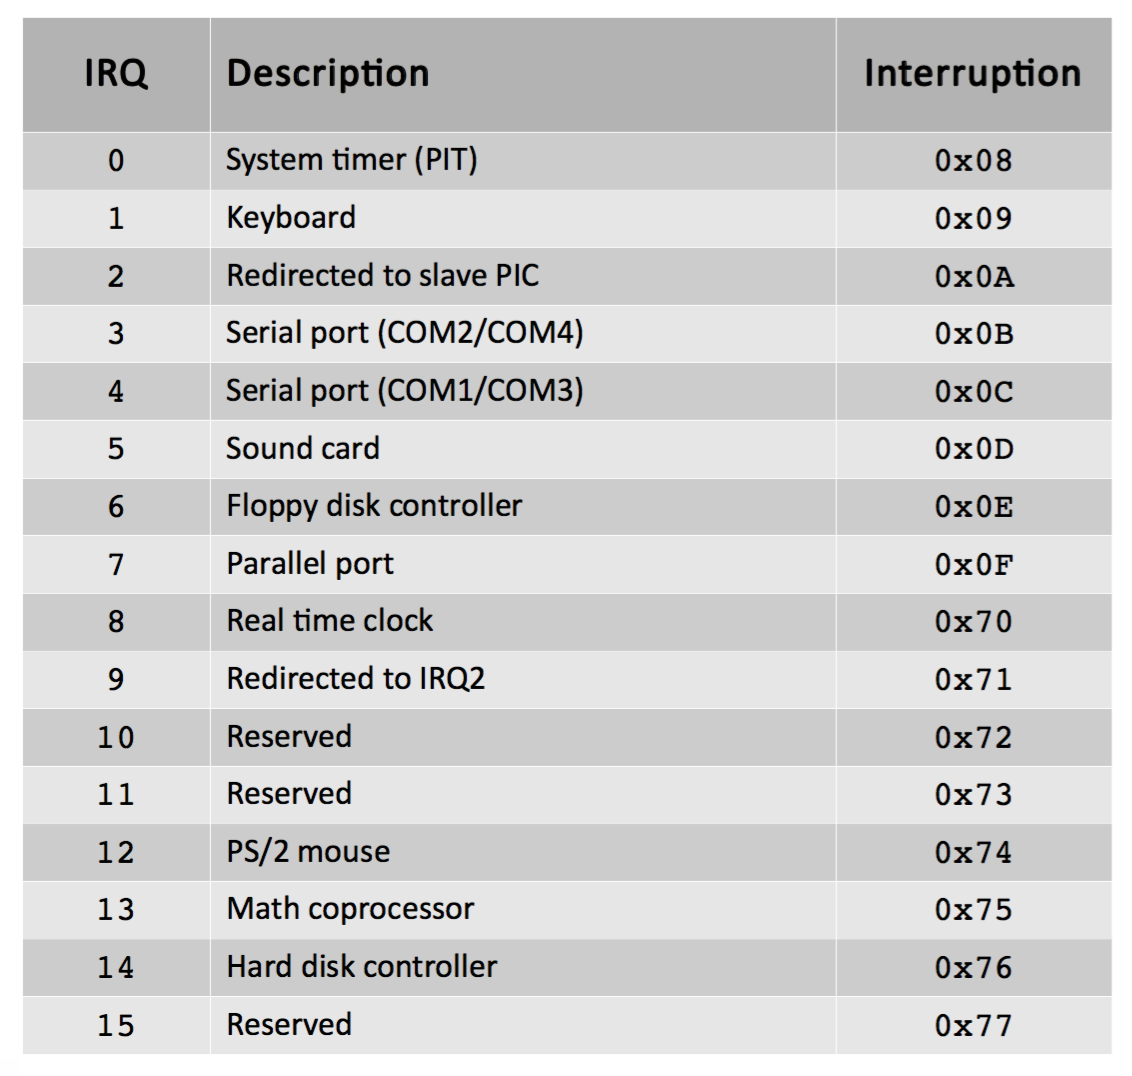
\includegraphics[scale=0.5]{images/irqs.png}
  \caption{Table de correspondance des \acrshort{irq}s}
  \label{irqs}
\end{figure}

En comparant la figure \ref{table_int_exc} avec la figure \ref{irqs}, on constate
que certaines \acrshort{irq}s partagent le même numéro d'interruption que des
exceptions. L'interruption du \textit{timer} par exemple a le même numéro d'interruption
que l'exception \textit{Double Fault} (0x8). Si on laisse le \textit{mapping} par
défaut, une interruption du \textit{timer} va déclencher une \textit{Double Fault}
ce qui n'est pas souhaitable. Il a donc été nécessaire de changer cette table
de correspondance. Les \acrshort{irq}s 0 à 7 ont été associées aux interruptions
32 à 39 et les \acrshort{irq}s 8 à 15 ont été associées aux interruptions 40 à 47.
Ce changement de \textit{mapping} peut se faire assez simplement en assembleur en
utilisant les ports des deux \acrshort{pic}s utilisés par les \acrshort{irq}s.
Un code d'exemple est donné sur le site OSDev.\cite{ref22}

%%%%%%%%%%%%%%%%%%%%%%%%%%%%%%%%%%%%%%%%%%%%%%%%%%%%%%%%%%%%%%%%%%

\subsubsection{\acrshort{idt}}
La table des descripteurs d'interruption (ou \acrshort{idt}) est similaire à la
\acrshort{gdt} (la table des descripteurs globaux). Elle est aussi composée de
descripteurs de 64-bits permettant chacun de référencer une interruption. Un
descripteur est composé d'un offset indiquant l'adresse de l'\acrshort{isr} (la
routine d'interruption), un selecteur de segment indiquant le segment où se trouve
le code de l'\acrshort{isr} et un niveau de privilège indiquant le niveau de privilège
requis pour exécuter l'\acrshort{isr}. Dans le cas d'un adressage de type \textit{FLAT}
comme celui utilisé, le selecteur de segment sera forcément le selecteur de segment
de code. Il existe aussi plusieurs types de descripteurs d'interruptions\cite{ref66}
décrits dans la figure \ref{idt_entry}. Dans le cas de notre \textit{kernel} seulement
deux types ont été utilisés, le type \textit{Interrupt Gate} et le type \textit{Trap Gate}.
La différence entre un \textit{Interrupt Gate} et un \textit{Trap Gate} est uniquement
le comportement du \acrshort{cpu} lors de l'exécution de l'\acrshort{isr}\cite{ref42}.
Dans le cas du \textit{Interrupt Gate}, le \acrshort{cpu} masquera les interruptions
lors de l'exécution de l'\acrshort{isr} alors que dans un \textit{Trap Gate} ce
ne sera pas le cas. \\

\begin{figure}[!h]
  \centering
  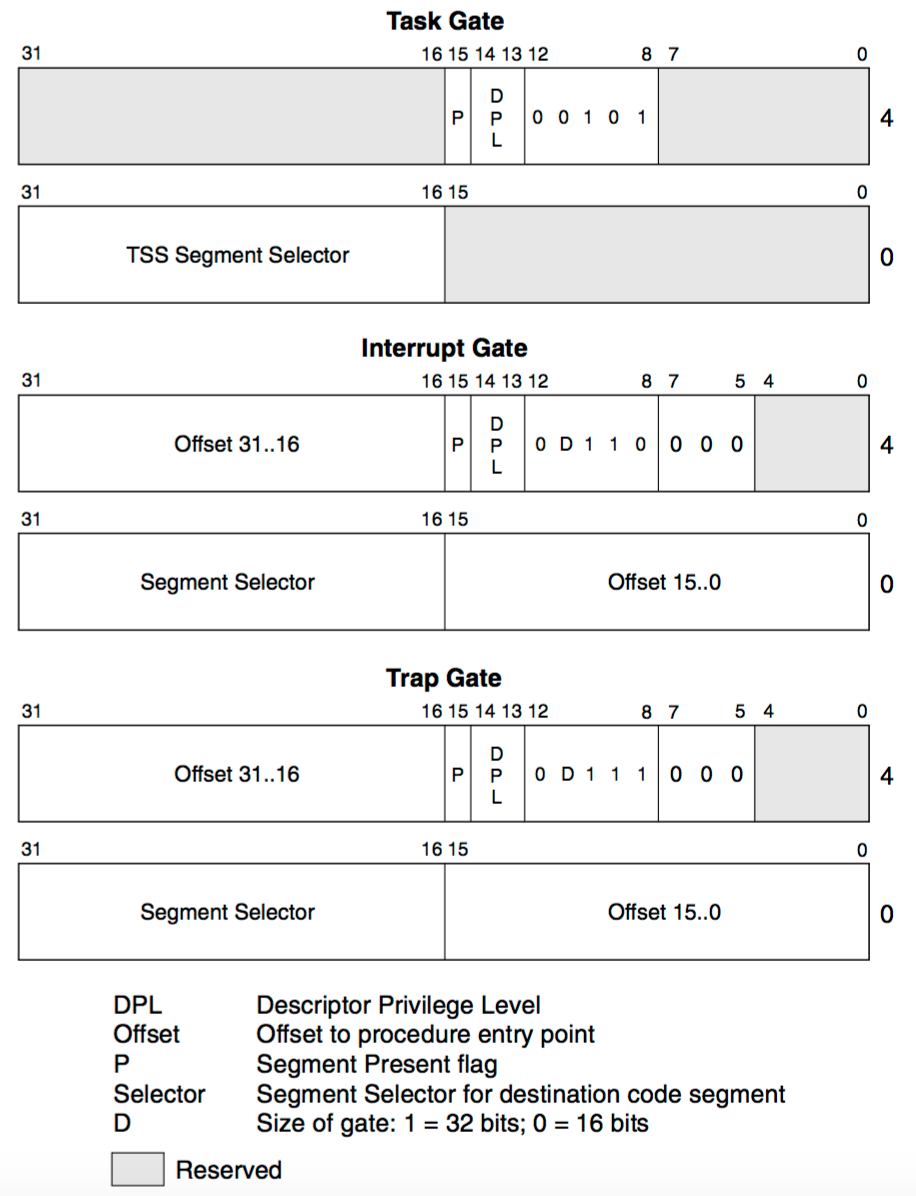
\includegraphics[scale=0.75]{images/idt_entry.png}
  \caption{Différents types de descripteur d'interruption}
  \label{idt_entry}
\end{figure}

Comme pour la \acrshort{gdt}, l'\acrshort{idt} est stockée en \acrshort{ram}
et doit donc être initialisée et gérée par l'\acrshort{os}. De la même manière
que l'instruction \mintinline{text}{LGDT} permet de charger la \acrshort{gdt},
l'instruction \mintinline{text}{LIDT} permet de charger l'\acrshort{idt} dans le
registre IDTR. Pour se faire il faut donner comme argument à l'instruction 
\mintinline{text}{LIDT} l'adresse du descripteur d'\acrshort{idt} sur 48 bits.
Ce descripteur est composé de l'adresse de l'\acrshort{idt} sur 32 bits et de sa
limite (sa taille en bytes - 1) sur 16 bits. Une fois la table des descripteurs
d'interruption chargée avec l'instruction \mintinline{text}{LIDT}, les interruptions
peuvent être activées en utilisant l'instruction \mintinline{text}{STI}. La figure
\ref{idtr} permet de résumer la relation entre le registre IDTR et l'\acrshort{idt}.

\begin{figure}[!h]
  \centering
  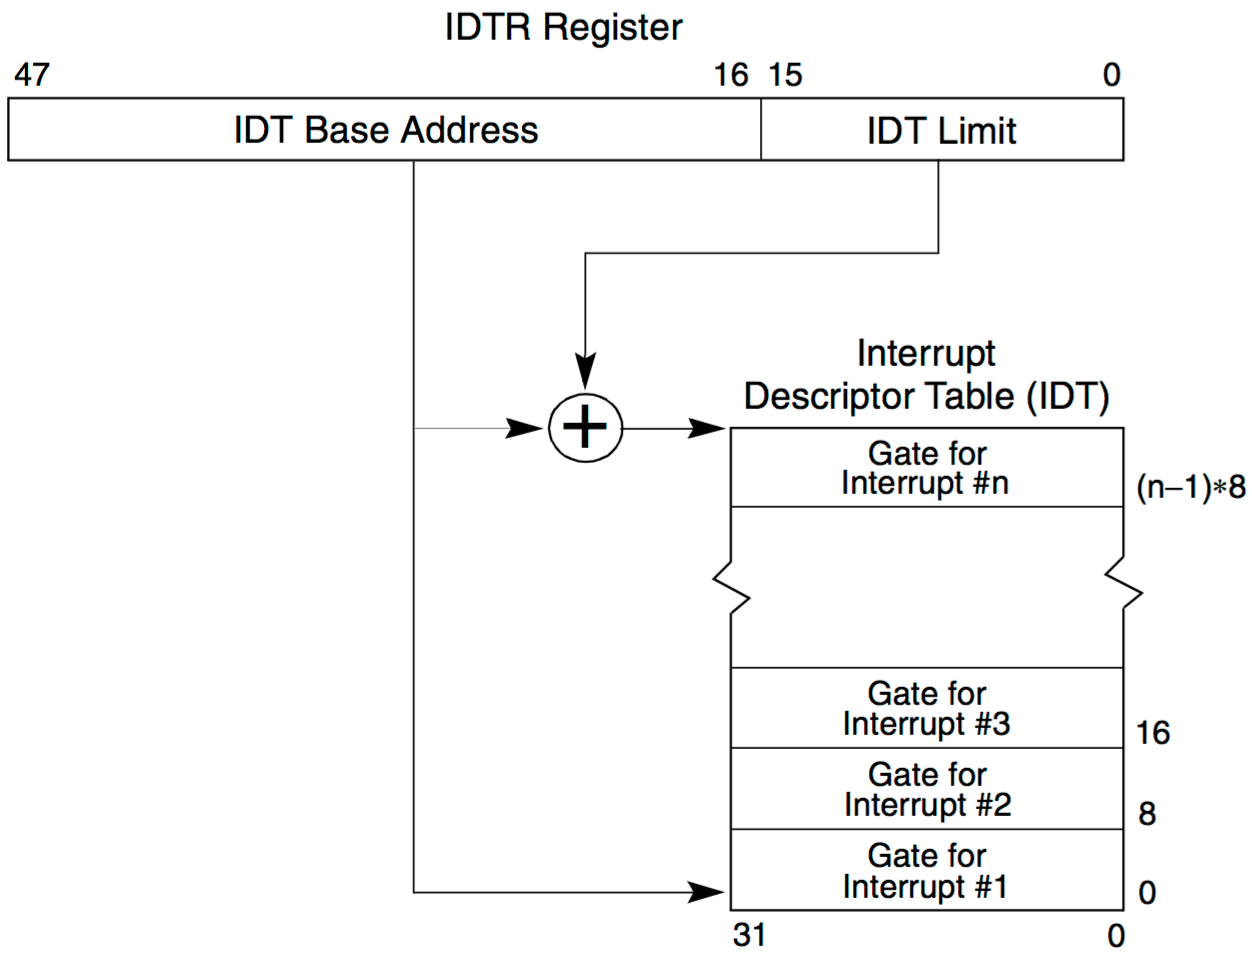
\includegraphics[scale=0.6]{images/idtr.png}
  \caption{Relation entre le registre IDTR et l'\acrshort{idt}}
  \label{idtr}
\end{figure}

Dans le \textit{kernel} développé, l'\acrshort{idt} est une structure statique
en mémoire. Une fonction assembleur est donc appelée afin de charger cette
structure dans le registre IDTR. En plus du chargement de l'\acrshort{idt}, une
partie des routines d'interruptions est faite en assembleur. En effet, il a été
nécéssaire de passer par du code bas niveau car avant de rentrer dans une
routine d'interruption, il faut sauvegarder le contexte. Il est obligatoire
de sauvegarder le contexte car, comme déjà dit plus haut, une interruption
peut avoir lieu à n'importe quel moment. La partie bas niveau de la routine
d'interruption s'occupe donc de sauvegarder le contexte puis d'appeler un
gestionnaire d'interruption haut niveau en rust. Ce gestionnaire prend comme argument
le numéro d'interruption et appelle la routine d'interruption liée à cette interruption.
Par exemple, la routine d'interruption du \textit{timer} va simplement incrémenter
un compteur. Lorsque une exception est levée le même mécanisme est employé sauf
qu'ici le \textit{kernel} va afficher un message d'erreur en fonction du numéro
de l'exception.

%%%%%%%%%%%%%%%%%%%%%%%%%%%%%%%%%%%%%%%%%%%%%%%%%%%%%%%%%%%%%%%%%%
%%%%%%%%%%%%%%%%%%%%%%%%%%%%%%%%%%%%%%%%%%%%%%%%%%%%%%%%%%%%%%%%%%

\subsection{\acrshort{vga}}
Un \acrshort{pc} possède généralement une carte graphique permettant de gérer
l'affichage. Une grande majorité des carte graphiques, même modernes sont compatibles
avec le standard d'affichage \acrshort{vga}. Dans notre cas, nous utilisons un
émulateur (QEMU) qui va émuler l'affichage \acrshort{vga}. Pour écrire sur l'écran
il faut écrire dans la mémoire vidéo (\acrshort{vram}) qui commence à l'adresse
0xA0000 et finit à l'adresse 0xBFFFF. Différents modes d'écriture existent pour
l'affichage mais nous allons nous concentrer sur un seul en particulier. \\

Le mode texte \acrshort{vga} a été utilisé pour l'affichage dans l'\acrshort{os}
développé. En mode texte, l'écran est divisé en caractères plutôt qu'en pixels ce
qui permet d'afficher simplement et rapidement quelque chose sur l'écran. La mémoire
vidéo reservée au mode texte commence à l'adresse 0xB8000 et a une taille de
$80 \times 25$ caractères. Un caractère est représenté par 2 octets (16 bits) ce
qui fait une taille de 4000 octets ($80 \times 25 \times 2$). L'octet de poids
faible d'un caractère représente la valeur ASCII de ce caractère et l'octet de poids
fort représente l'attribut qui contient lui même la couleur du caractère et la
couleur du fond (voir figure \ref{vga_char}) \cite{ref42}. La couleur en mode texte
est donc codée sur 4 bits ce qui fait 16 couleurs différentes. Ces 16 couleurs sont
décrites dans la figure \ref{colors} \cite{ref19}. \\

\begin{figure}[!h]
  \centering
  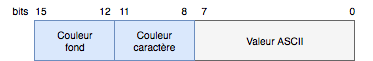
\includegraphics[scale=0.8]{images/vga_char.png}
  \caption{Structure d'un caractère en mode texte \acrshort{vga}}
  \label{vga_char}
\end{figure}

\begin{figure}[!h]
  \centering
  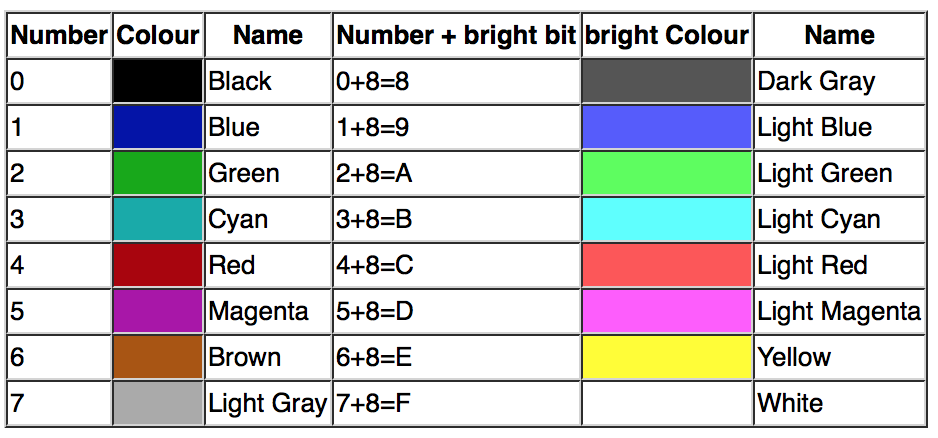
\includegraphics[scale=0.7]{images/colors.png}
  \caption{Couleurs disponibles en mode texte \acrshort{vga}}
  \label{colors}
\end{figure}

Le mode texte \acrshort{vga} permet aussi d'afficher un curseur. Le curseur ne
se déplace pas automatiquement quand un caractère est écrit à l'écran, c'est
simplement une zone de l'écran mise en évidence par un clignotement et dont
la taille, la position et la visibilité peuvent être modifiés \cite{ref23}. L'accès
au curseur se fait en utilisant les registres du \acrshort{crtc} (\textit{Cathode Ray
Tube Controller}). Les registres du \acrshort{crtc} peuvent être accédés avec la
paire registre d'adresse et registre de données. Ces regsitres se trouvent respectivement
aux ports 0x3D4 et 0x3D5. L'écriture dans un registre du \acrshort{crtc} se fait
donc en deux temps. Tout d'abord, l'adresse du registre doit être specifiée
en écrivant dans le port 0x3D4 puis la donnée doit être écrite dans le port 0x3D5
\cite{ref42}.

%%%%%%%%%%%%%%%%%%%%%%%%%%%%%%%%%%%%%%%%%%%%%%%%%%%%%%%%%%%%%%%%%%
%%%%%%%%%%%%%%%%%%%%%%%%%%%%%%%%%%%%%%%%%%%%%%%%%%%%%%%%%%%%%%%%%%

\subsection{\textit{Timer}}

%%%%%%%%%%%%%%%%%%%%%%%%%%%%%%%%%%%%%%%%%%%%%%%%%%%%%%%%%%%%%%%%%%
%%%%%%%%%%%%%%%%%%%%%%%%%%%%%%%%%%%%%%%%%%%%%%%%%%%%%%%%%%%%%%%%%%

\subsection{Clavier}

%%%%%%%%%%%%%%%%%%%%%%%%%%%%%%%%%%%%%%%%%%%%%%%%%%%%%%%%%%%%%%%%%%
%%%%%%%%%%%%%%%%%%%%%%%%%%%%%%%%%%%%%%%%%%%%%%%%%%%%%%%%%%%%%%%%%%

\newpage
\section{Système de fichiers}
%%%%%%%%%%%%%%%%%%%%%%%%%%%%%%%%%%%%%%%%%%%%%%%%%%%%%%%%%%%%%%%%%%
%%%%%%%%%%%%%%%%%%%%%%%%%%%%%%%%%%%%%%%%%%%%%%%%%%%%%%%%%%%%%%%%%%

\subsection{Introduction}

%%%%%%%%%%%%%%%%%%%%%%%%%%%%%%%%%%%%%%%%%%%%%%%%%%%%%%%%%%%%%%%%%%
%%%%%%%%%%%%%%%%%%%%%%%%%%%%%%%%%%%%%%%%%%%%%%%%%%%%%%%%%%%%%%%%%%

\subsection{Structure}


%%%%%%%%%%%%%%%%%%%%%%%%%%%%%%%%%%%%%%%%%%%%%%%%%%%%%%%%%%%%%%%%%%
%%%%%%%%%%%%%%%%%%%%%%%%%%%%%%%%%%%%%%%%%%%%%%%%%%%%%%%%%%%%%%%%%%

\newpage
\section{Tâches utilisateurs}
\label{user}
%%%%%%%%%%%%%%%%%%%%%%%%%%%%%%%%%%%%%%%%%%%%%%%%%%%%%%%%%%%%%%%%%%
%%%%%%%%%%%%%%%%%%%%%%%%%%%%%%%%%%%%%%%%%%%%%%%%%%%%%%%%%%%%%%%%%%

\subsection{Introduction}
En mode protégé (architecture Intel 32 bits, \acrshort{IA-32}), quatre niveaux
de privilèges existent.
Nous avons déjà fait référence aux niveaux de privilèges (ou \textit{ring})
dans ce document quand les différentes tables de descripteurs ont été décrites
(chapitres \ref{gdt_ldt} sur la \acrshort{gdt} et la \acrshort{ldt} et \ref{idt}
sur l'\acrshort{idt}). Les niveaux de privilèges vont de 0 à 3. Le \textit{ring}
0 (\textit{kernel}) a le plus de privilèges et peut accéder à tout le jeu d'instructions
du processeur alors que le \textit{ring} 3 (\textit{user}) en a le moins et a accès
à un jeu d'instructions restreint \cite{ref42}.

\begin{figure}[!h]
  \centering
  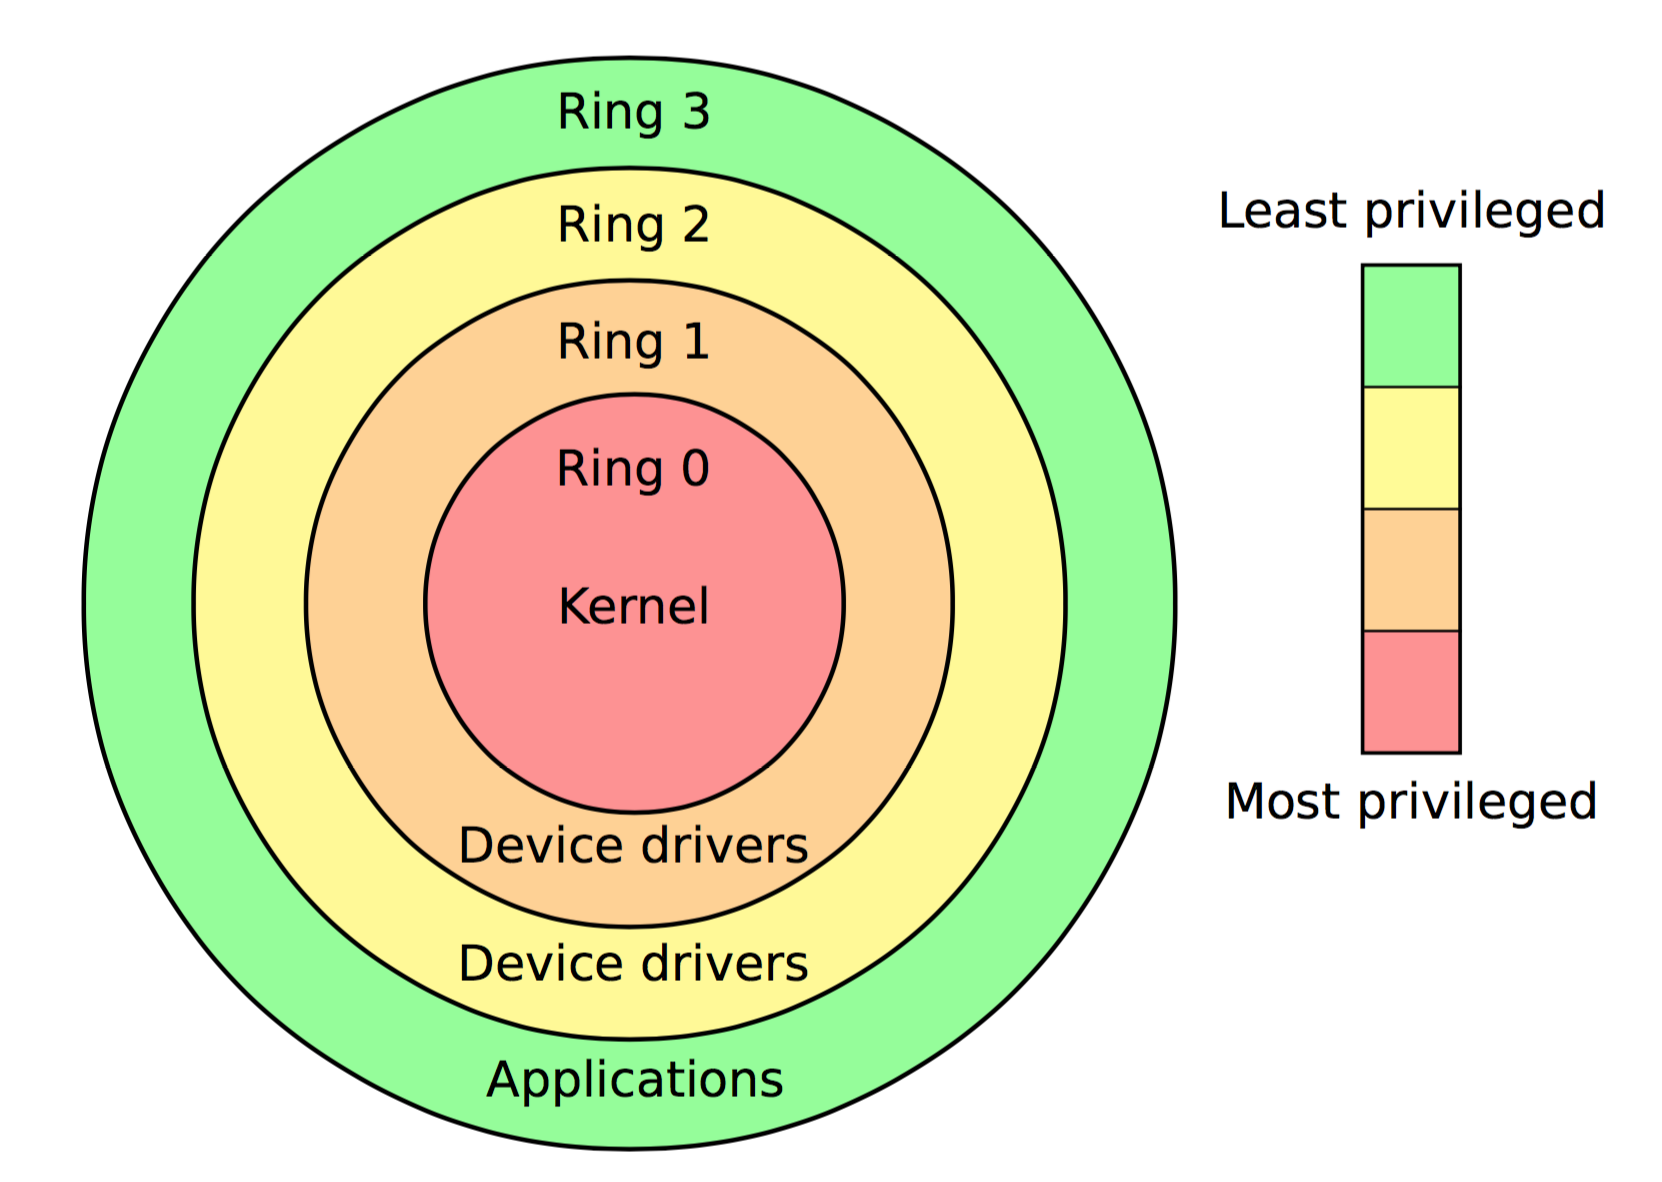
\includegraphics[scale=.4]{images/rings.png}
  \caption{Niveaux de privilèges sur architecture \acrshort{IA-32}}
  \label{rings}
\end{figure}

Le \textit{ring} 0 est aussi appelé mode privilégié. Ce mode peut accéder aux régions
privilégiées de la mémoire (définies lors de l'initialisation de la \acrshort{gdt}
ou de la pagination). Seulement ce mode peut contrôler le \acrshort{mmu}, accéder
aux périphériques, définir les vecteurs d'interruptions ou encore arrêter le
processeur. L'\acrshort{os} démarre en mode privilégié car le \textit{kernel} doit
pouvoir accéder au matériel sans aucune restriction. Si ce n'était pas le cas toutes
les configurations de la mémoire et des périphériques décrites dans ce document
auraient été impossibles. En revanche, Les applications utilisateurs s'exécutent
en mode utilisateur (\textit{ring} 3). Si une application utilisateur démarrait
avec le niveau de privilèges maximal, elle pourrait écrire dans les régions mémoires
du \textit{kernel}, modifier la configuration de la mémoire (\acrshort{gdt} ou 
répertoire de pages) ou encore changer l'\acrshort{idt}. Il est donc impératif
d'exécuter les applications en \textit{ring} 3. Grâce à ce mécanisme de protection,
le \textit{kernel} peut être complètement isolé des applications. Le rôle du \textit{kernel}
est d'abord d'attribuer et de gérer l'espace mémoire de chaque application.
Il doit ensuite programmer correctement le processeur pour isoler les tâches exécutées
et assurer le bon fonctionnement du système.

%%%%%%%%%%%%%%%%%%%%%%%%%%%%%%%%%%%%%%%%%%%%%%%%%%%%%%%%%%%%%%%%%%
%%%%%%%%%%%%%%%%%%%%%%%%%%%%%%%%%%%%%%%%%%%%%%%%%%%%%%%%%%%%%%%%%%

\subsection{Exécution d'une tâche}
\subsubsection{Structure d'une tâche}
L'architecture \acrshort{IA-32} implémente la gestion des tâches au niveau matériel.
Une tâche doit être constituée d'un espace d'exécution et d'une structure \acrshort{tss}.
L'espace d'exécution est constitué d'un segment de code, d'un segment de données
et d'un segment de pile. La manière dont ces segments sont définis dépend de la
méthode de gestion mémoire utilisée. Si la pagination n'est pas utilisée, ces segments
seront définis par une \acrshort{ldt}. Avant d'implémenter la pagination, cette
méthode était utilisée par notre \textit{kernel} pour gérer l'espace d'adressage
d'une tâche. Avec la pagination, deux segments en \textit{ring} 3 sur tout l'espace
d'adressage suffisent (un segment de code et un segment de données). Ces segments
sont identiques à ceux déjà construits pour le \textit{kernel} et décrits dans
la partie \ref{gdt_ldt} à la différence qu'ils n'ont pas le même niveau de privilèges.
Ainsi, une tâche a théoriquement un espace d'exécution de 4Go (taille de la \acrshort{ram}).
En réalité, l'espace d'exécution de la tâche est défini par un répertoire de pages
(différent de celui du \textit{kernel}) où seront allouées autant de pages qu'il faut
pour contenir l'application utilisateur. C'est la structure \acrshort{tss} qui spécifie
les segments définissant l'espace d'exécution. Si la pagination n'est pas utilisée,
c'est dans cette structure que le sélecteur vers la \acrshort{ldt} doit être spécifié.
Dans le cas contraire, le \acrshort{tss} contient aussi un champs \mintinline{rust}{cr3}
pour définir le répertoire de pages de la tâche (voir figure \ref{task_exec_space})
\cite{ref66}.

\begin{figure}[!h]
  \centering
  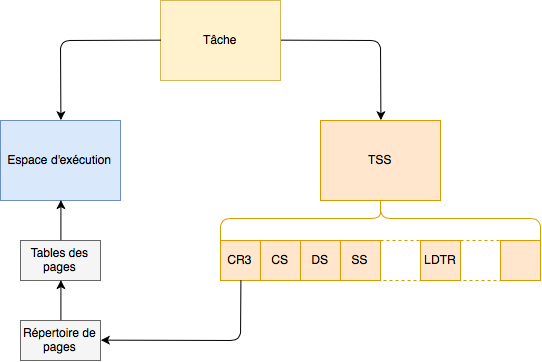
\includegraphics[scale=.7]{images/task_exec_space.png}
  \caption{Structure d'une tâche avec la pagination}
  \label{task_exec_space}
\end{figure}

La structure \acrshort{tss} permet aussi de sauvegarder le contexte de la tâche
dans le cas où une tâche en appelle une autre. Chaque \acrshort{tss} a un descripteur
dans la \acrshort{gdt}. Il y a donc autant de descripteurs de \acrshort{tss} dans
la \acrshort{gdt} que de tâches. Une tâche est alors identifiée par le sélecteur
de segment référençant son \acrshort{tss} dans la \acrshort{gdt} \cite{ref42}. Etant
donné que la pagination est utilisée dans la version finale de notre \acrshort{os},
nous allons nous concentrer sur la gestion des tâches utilisant un répertoire de
pages.

%%%%%%%%%%%%%%%%%%%%%%%%%%%%%%%%%%%%%%%%%%%%%%%%%%%%%%%%%%%%%%%%%%

\subsubsection{Commutation de tâches}
Nous avons vu dans la partie précédente qu'une tâche est divisée en deux parties,
son espace d'exécution et sa structure \acrshort{tss}. Le processeur fourni un
mécanisme permettant de sauvegarder le contexte de la tâche courante et de commuter
vers une nouvelle tâche. La sauvegarde du contexte se fait en utilisant le \acrshort{tss}
lié à la tâche à exécuter et plus particulièrement le sélecteur de ce \acrshort{tss}
dans la \acrshort{gdt}. Ce dernier doit être donné comme argument à l'instruction
\mintinline{text}{ltr}. Cette instruction permet de charger le sélecteur de \acrshort{tss}
dans un registre spécial, le \textit{task register}. Ce registre indique au processeur
quelle est la tâche courante. Lorsqu'une commutation de tâche a lieu, l'état
courant du processeur est automatiquement sauvegardé dans le \acrshort{tss} pointé
par le \textit{task register}. Il est donc nécessaire de créer un \acrshort{tss}
initial avant d'exécuter la première tâche car l'état du processeur doit être
sauvegardé \cite{ref42}. Ci-dessous, la structure \acrshort{tss} en rust.

\begin{code}
\begin{minted}[fontsize=\footnotesize,tabsize=4,frame=single,linenos]{rust}
pub struct Tss {
    previous_task_link : u16, reserved0    : u16,
    esp0               : u32,
    ss0                : u16, reserved1    : u16,
    esp1               : u32,
    ss1                : u16, reserved2    : u16,
    esp2               : u32,
    ss2                : u16, reserved3    : u16,
    cr3                : u32,
    eip                : u32, eflags       : u32, eax: u32, ecx: u32, edx: u32,
    ebx                : u32, esp          : u32, ebp: u32, esi: u32, edi: u32,
    es                 : u16, reserved4    : u16,
    cs                 : u16, reserved5    : u16,
    ss                 : u16, reserved6    : u16,
    ds                 : u16, reserved7    : u16,
    fs                 : u16, reserved8    : u16,
    gs                 : u16, reserved9    : u16,
    ldt_selector       : u16, reserved10   : u16,
    reserved11         : u16,
    iomap_base_addr    : u16
}
\end{minted}
\caption{Champs de la structure \acrshort{tss}}
\label{lst:tasks:tss}
\end{code} \bigbreak

Dans le \acrshort{tss} initial, seuls les champs \mintinline{rust}{esp0},
\mintinline{rust}{ss0} et \mintinline{rust}{cr3} sont utilisés. Les champs
\mintinline{rust}{esp0} et \mintinline{rust}{ss0} sont utilisés pour stocker
la pile pour le niveau de privilèges 0 et \mintinline{rust}{cr3} doit pointer
sur le répertoire de pages du \textit{kernel}. Ce \acrshort{tss} est ensuite chargé
dans le \textit{task register} avec l'instruction \mintinline{text}{ltr}. Le
\textit{kernel} peut maintenant exécuter une tâche utilisateur. L'architecture
\acrshort{IA-32} offre de nombreux mécanismes pour commuter vers une nouvelle
tâche. La méthode utilisée est un appel explicite à la tâche avec l'instruction
\mintinline{text}{call far}. Cette instruction prend comme argument le sélecteur
du \acrshort{tss} de la tâche à exécuter (comme l'instruction \mintinline{text}{ltr}).
L'initialisation du \acrshort{tss} d'une tâche est légèrement plus complexe que
celle du \acrshort{tss} initial. Les sélecteurs de segment doivent pointer sur les
bons segments dans la \acrshort{gdt}. De plus, le pointeur d'exécution doit
pointer là où commence le code du programme utilisateur et les champs \mintinline{rust}{ss},
\mintinline{rust}{esp} et \mintinline{rust}{ebp} sont utilisés pour stocker la pile
pour le niveau de privilèges 3. L'adresse du début du programme utilisateur dépend
de la manière dont le répertoire de pages de la tâche a été initialisé. Dans notre
cas, le programme utilisateur commence toujours à l'adresse 0x0. Un programme
utilisateur contenu par exemple dans le disque dur peut ainsi être exécuté en
\textit{ring} 3.

%%%%%%%%%%%%%%%%%%%%%%%%%%%%%%%%%%%%%%%%%%%%%%%%%%%%%%%%%%%%%%%%%%
%%%%%%%%%%%%%%%%%%%%%%%%%%%%%%%%%%%%%%%%%%%%%%%%%%%%%%%%%%%%%%%%%%

\subsection{Appels systèmes}
Les appels systèmes sont des fonctions exposées aux applications utilisateurs par
le \textit{kernel}. Lors d'un appel système, un changement de privilèges a lieu
car du code du \textit{kernel} est appelé. Il est important d'avoir des appels
systèmes dans un \textit{kernel} appelant des applications utilisateurs.
Un programme utilisateur ne pourrait que modifier des variables et appeler des
fonctions s'il ne pouvait pas appeler du code au niveau du \textit{kernel}. Prenons
par exemple un simple affichage texte. Le programme utilisateur étant isolé du reste
de la mémoire, il ne peut pas accéder à la \acrshort{vram} et par conséquent ne
peut rien afficher à l'écran. Les appels systèmes se présentent donc comme une
\acrshort{api} de l'\acrshort{os}. Le mécanisme permettant au code exécuté en
mode utilisateur d'appeler du code en mode \textit{kernel}
est réalisé grâce à une interruption logicielle choisie et configurée par le \textit{kernel}.
Cette interruption est configurée afin d'être exécutable en \textit{ring} 3.
Dans le cas de notre \textit{kernel}, l'interruption utilisée est la première libre
après les interruptions matérielles. C'est l'interruption 48. Sa configuration se
fait avec le code rust ci-dessous.

\begin{code}
\begin{minted}[fontsize=\footnotesize,tabsize=4,frame=single,linenos]{rust}
IDT[48] = IdtEntry::new(GDT_KERNEL_CODE_SELECTOR as u16,
                        _syscall_handler as *const () as u32,
                        TYPE_TRAP_GATE, DPL_USER);
\end{minted}
\caption{Entrée dans l'\acrshort{idt} pour les appels systèmes}
\label{lst:tasks:syscalls:idtentry}
\end{code} \medbreak

La structure des entrées de l'\acrshort{idt} est décrite dans la figure \ref{idt_entry}.
Dans ce code, le constructeur d'une entrée prend comme arguments : le sélecteur de
segment pour accéder à l'\acrshort{isr} (ici le sélecteur de segment de code du
\textit{kernel}), le pointeur vers l'\acrshort{isr} en question, le type d'entrée
(ici c'est une \textit{trap gate}) et enfin le niveau de privilèges pour appeler
cette interruption. Ainsi, cette interruption peut être appelée avec l'instruction
\mintinline{text}{INT 48}. A noter qu'une seule interruption logicielle gère tous
les appels systèmes. Ceci est possible car un numéro d'appel système est passé en
argument à la routine d'interruption qui s'occupe d'appeler la bonne fonction.
En général, d'autres paramètres doivent être passés à l'appel système dépendamment
de l'action faite par ce dernier. Par exemple une chaîne de caractères à afficher
à l'écran. Tous ces paramètres sont envoyés à la routine d'interruption dans les
registres du processeur (\mintinline{text}{eax}, \mintinline{text}{ebx}, \mintinline{text}{ecx},
\mintinline{text}{edx} et \mintinline{text}{esi}).

\begin{figure}[!h]
  \centering
  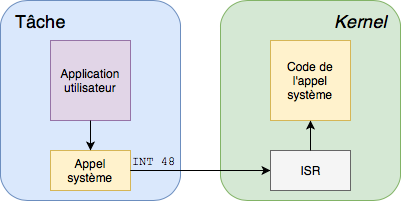
\includegraphics[scale=.7]{images/syscall.png}
  \caption{Fonctionnement des appels systèmes}
  \label{syscall}
\end{figure}

Avec la pagination active, il est important de copier les tables des pages et les
pages du \textit{kernel} dans le répertoire de pages de la tâche. C'est pour cette
raison que nous avons déplacé le \textit{kernel} dans le dernier gigaoctet de
\acrshort{ram} (chapitre \ref{activate_paging}). De cette façon, les trois premiers
gigaoctets de \acrshort{ram} peuvent être utilisés par une application utilisateur
et le reste par le \textit{kernel}.

%%%%%%%%%%%%%%%%%%%%%%%%%%%%%%%%%%%%%%%%%%%%%%%%%%%%%%%%%%%%%%%%%%
%%%%%%%%%%%%%%%%%%%%%%%%%%%%%%%%%%%%%%%%%%%%%%%%%%%%%%%%%%%%%%%%%%

\subsection{Allocation dynamique en mode utilisateur}
\label{alloc_user}
Le concept d'allocation dynamique a été expliqué dans le chapitre \ref{alloc_kernel}.
Les fonction décrites dans ce chapitre permettent seulement d'allouer de la mémoire
en mode \textit{kernel}. Les tâches utilisateurs pourraient très bien se passer
d'allocation dynamique et utiliser des structures statiques à la place. C'est
d'ailleurs de cette manière qu'avaient été implémentées les tâches dans une version
précédente de l'\acrshort{os}. Le problème avec l'utilisation de structures
statiques est que la même quantité de mémoire va être utilisée pour une application
faisant 200 octets et une application faisant 200'000 octets. De plus, toute la
mémoire dédiée aux tâches doit alors être réservée dès la compilation du \textit{kernel}
ce qui augmente très rapidement sa taille. Un autre avantage à allouer la mémoire
dynamiquement en \textit{ring} 3 est que des fonctions d'allocation dynamique 
peuvent alors être implémentées au niveau utilisateur (comme \mintinline{c}{malloc}
et \mintinline{c}{free}). \\

Dans le chapitre \ref{alloc_kernel}, nous avons vu les structures et mécanismes
mis en place pour allouer de la mémoire dynamiquement en mode \textit{kernel}.
Des fonctions supplémentaires ont été implémentées pour gérer la mémoire dynamique en
mode \textit{user}. Ces fonctions sont \mintinline{rust}{umalloc} et
\mintinline{rust}{ufree}. La fonction \mintinline{rust}{umalloc} alloue d'abord
de la mémoire en \textit{ring} 0 puis \textit{map} ces blocs mémoire
dans le répertoire de pages de la tâche utilisateur en commençant à l'adresse 0x0.
Le code du programme utilisateur est donc situé physiquement dans le \textit{heap}
du \textit{kernel} mais est placé virtuellement au début de l'espace d'adressage
de la tâche. Ce mécanisme est expliqué par la figure \ref{mem_view_user}.
Dans cet exemple, on peut voir que le code du programme utilisateur se situe
dans le tas du \textit{kernel} mais qu'il est \textit{mappé} à l'adresse 0x0
dans l'espace d'adressage de la tâche. A noter que le \textit{kernel} et son tas
sont encore présents dans la mémoire en mode \textit{user} pour rendre possibles
les appels systèmes.

\begin{figure}[!h]
  \centering
  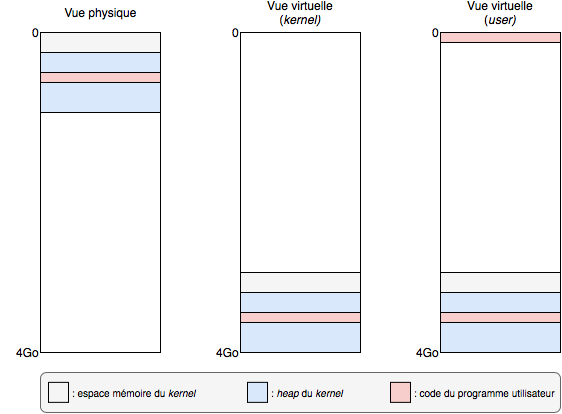
\includegraphics[scale=.7]{images/alloc_user.png}
  \caption{Vues de la mémoire après allocation d'un code utilisateur}
  \label{mem_view_user}
\end{figure}

%%%%%%%%%%%%%%%%%%%%%%%%%%%%%%%%%%%%%%%%%%%%%%%%%%%%%%%%%%%%%%%%%%
%%%%%%%%%%%%%%%%%%%%%%%%%%%%%%%%%%%%%%%%%%%%%%%%%%%%%%%%%%%%%%%%%%

\subsection{Librairie système et applications}
\subsubsection{Compilation d'une application utilisateur}
\label{sec:user:compil}
Le \textit{kernel} pouvant charger et exécuter des programmes, les appels systèmes
étant mis en place et l'allocation dynamique fonctionnelle en mode \textit{user},
des programmes utilisateurs peuvent maintenant être écrits. Ces applications
sont compilées séparément du \textit{kernel} avec un \textit{linker} qui leur
est propre. D'ailleurs, une application peut être codée dans le langage voulu
tant que le \textit{linker} fourni est utilisé. Un programme utilisateur est
compilé en format binaire. Sous ce format, le code du programme commence directement
à l'adresse 0x0. Il n'y a pas d'entête comme avec le format \acrshort{elf}.
Ci-dessous, les lignes importantes du \textit{linker} pour compiler en format
binaire. Ce \textit{linker} appelle une fonction assembleur très simple qui
appelle la fonction \mintinline{rust}{main} du programme \cite{ref42}.

\begin{code}
\begin{minted}[fontsize=\footnotesize,tabsize=4,frame=single,linenos]{text}
OUTPUT_FORMAT("binary")
SECTIONS {
    . = 0x0;
    ...
}
\end{minted}
\caption{\textit{Linker} pour un exécutable en format binaire}
\label{lst:tasks:app:linker}
\end{code} \bigbreak

Le langage Rust a été utilisé pour développer une librairie système et quelques
applications. La compilation de Rust est légèrement différente que pour le
\textit{kernel}. D'une part nous sommes dans un format binaire, et ensuite
il faut se défaire de tous les mécanismes de protection de Rust qui prennent
une place considérable dans l'exécutable. Pour compiler un programme Rust
en fichier objet destiné à un format binaire, le \textit{flag}
\mintinline{text}{-C relocation-model=static} doit être passé au compilateur.
Par défaut, le compilateur cherche la \mintinline{text}{GLOBAL_OFFSET_TABLE}
qui n'existe pas lorsque le format de l'exécutable est un format binaire.
Ce \textit{flag} va dire au compilateur d'ignorer ce mécanisme \cite{ref25}.
De cette façon, un programme utilisateur peut être compilé mais sa taille sera
excessivement grande (de l'ordre des 100'000 octets). Ceci est dû à plusieurs
raisons. Tout d'abord, Rust est compilé par défaut sans aucune option d'optimisation.
Le \textit{flag} \mintinline{text}{-C opt-level=3} fixe un niveau d'optimisation
de 3 (plus haut niveau d'optimisation). Un peu plus d'optimisation peut être
fait en demandant à Xargo de compiler en mode \textit{release} et non \textit{debug}
avec l'option \mintinline{text}{--release}. Le niveau d'optimisation a un impact
sur le code écrit mais ce sont les librairies qui prennent le plus de place dans
un exécutable. Pour rappel, nous compilons sans librairie standard mais la librairie
\mintinline{text}{core} est tout de même utilisée. Quand on compile un code Rust,
l'intégralité de cette librairie est également compilée, même si certaines parties
sont inutiles. Pour résoudre ce problème il faut cette fois-ci modifier le fichier
\mintinline{text}{cargo.toml} et lui rajouter les lignes suivantes \cite{ref26}.

\begin{code}
\begin{minted}[fontsize=\footnotesize,tabsize=4,frame=single,linenos]{text}
[profile.release]
lto = true
panic = 'abort'
\end{minted}
\caption{Options ajoutées au fichier \mintinline{text}{cargo.toml}}
\label{lst:tasks:app:cargotoml}
\end{code} \bigbreak

A noter que les \textit{flags} passés au compilateur de Rust (avec l'option
\mintinline{text}{-C}), sont appliqués au compilateur rustc et non à Xargo. Pour
dire à Xargo (ou Cargo) de rajouter des options lors de la compilation, il faut
mettre ces options dans la variable d'environnement \mintinline{text}{RUSTFLAGS}.
Comme pour le \textit{kernel}, \acrshort{gcc} est utilisé pour \textit{linker}
les fichier objets en un exécutable.

\subsubsection{Librairie système}
Pour faciliter le développement d'applications pour l'\acrshort{os}, une librairie
système a été développée. Cette dernière agit comme une mini librairie C offrant
les fonctionnalités de base à un programme utilisateur. Cette librairie offre
un niveau d'abstraction plus élevé cachant l'utilisation d'appels systèmes
à l'utilisateur. Ainsi, aucune application n'a besoin de faire appel des appels
systèmes. C'est la librairie système qui s'en charge. La librairie développée
offre les fonctionnalités suivantes.

\begin{center}
	\scalebox{1}{
		\begin{tabular}{| l | l |}
			\hline
			Fonction & Description \\ \hline
			\mintinline{rust}{print}/\mintinline{rust}{println} & Macros permettant
            d'afficher une chaîne de caractères formatée \\ \hline
			\mintinline{rust}{clear} & Efface l'écran \\ \hline
			\mintinline{rust}{puts} & Affiche une chaîne de caractères \\ \hline
			\mintinline{rust}{putc} & Affiche un caractère \\ \hline
			\mintinline{rust}{exec} & Exécute un programme utilisateur contenu
            dans le disque dur \\ \hline
            \mintinline{rust}{keypressed} & Indique si une touche du clavier a
            été appuyée \\ \hline
            \mintinline{rust}{getc} & Fonction bloquante. Retourne la touche
            appuyée par l'utilisateur \\ \hline
            \mintinline{rust}{file_stat} & Retourne les métadonnées d'un fichier \\ \hline
            \mintinline{rust}{file_open} & Ouvre un fichier donné en paramètre
            et retourne son descripteur \\ \hline
            \mintinline{rust}{file_close} & Ferme un fichier à partir de son
            descripteur \\ \hline
            \mintinline{rust}{file_read} & Lit les octets d'un fichier depuis son
            descripteur \\ \hline
            \mintinline{rust}{file_seek} & Avance le curseur d'un fichier depuis
            son descripteur \\ \hline
            \mintinline{rust}{file_iterator} & Retourne un itérateur des fichiers
            du disque dur \\ \hline
            \mintinline{rust}{file_next} & Itère sur le prochain fichier du disque \\ \hline
            \mintinline{rust}{get_ticks} & Retourne l'état actuel du \textit{timer} \\ \hline
            \mintinline{rust}{sleep} & Arrête l'exécution pendant un temps donné \\ \hline
            \mintinline{rust}{set_cursor} & Fixe la position du curseur sur l'écran \\ \hline
            \mintinline{rust}{get_cursor} & Retourne la position du curseur sur
            l'écran \\ \hline
            \mintinline{rust}{cursor_disable} & Active ou désactive le curseur \\ \hline
            \mintinline{rust}{copy_scr} & Copie un \textit{frame buffer} sur
            l'écran \\ \hline
            \mintinline{rust}{malloc} & Alloue de la mémoire \\ \hline
            \mintinline{rust}{free} & Libère de la mémoire \\ \hline
		\end{tabular}
	}
    \captionof{table}{Fonctions proposées par la librairie système}
    \label{tab:tasks:ulibc}
\end{center}

La fonction \mintinline{rust}{malloc} utilise un appel système allouant une nouvelle
page dans le répertoire de pages de la tâche. Cet appel système appelle lui même
la fonction \mintinline{rust}{umalloc} décrite dans la partie \ref{alloc_user}.
la fonction \mintinline{rust}{malloc} gère la mémoire de la même manière que le
\textit{kernel}. Un tas est utilisé au niveau utilisateur. Quand un utilisateur
alloue de la mémoire, \mintinline{rust}{malloc} regarde s'il y a assez de
place dans la dernière page allouée. Si c'est le cas, aucun appel système n'est
appelé, une partie de la dernière page va être reservée. Dans le cas contraire,
l'appel système pour allouer une page est appelé autant de fois que nécessaire.
Cette gestion utilise des entêtes qui fonctionnent exactement comme ceux du
\textit{heap} du \textit{kernel} décrits en \ref{alloc_kernel}. La seule différence
est que l'espace alloué n'est pas aligné sur 4096 octets (la taille d'une page)
car l'utilisateur aura tendance à allouer des espaces plus petits et cela produirait
une trop grande perte de mémoire. De plus, si l'espace alloué était aligné sur
la taille d'une page, un appel système aurait lieu à chaque allocation ce qui n'est
pas souhaitable.

\subsubsection{Applications développées}
\paragraph{Shell} \mbox{} \\
Actuellement, les applications utilisateurs ne peuvent être appélées que depuis
le \textit{kernel}. Ceci n'est pas pratique d'un point de vue utilisateur.
Afin d'avoir un système d'exploitation un peu plus interactif, un shell très
simple a été développé. Ce shell permet de lire les fichiers du disque dur et
d'exécuter d'autres applications utilisateurs. Le shell implémenté propose
les fonctionallités suivantes.

\begin{itemize}[label=\textbullet]
	\item \mintinline{text}{ls}         : liste les fichiers du disque dur
	\item \mintinline{text}{cat <file>} : affiche le contenu d'un fichier
	\item \mintinline{text}{clear}      : efface l'écran
	\item \mintinline{text}{<prog>}     : exécute un programme
    \item \mintinline{text}{sleep <ms>} : attend pendant un temps donné 
    \item \mintinline{text}{exit}       : sort du shell
    \item \mintinline{text}{help}       : affiche la liste des commandes disponibles
\end{itemize}

\begin{figure}[!h]
  \centering
  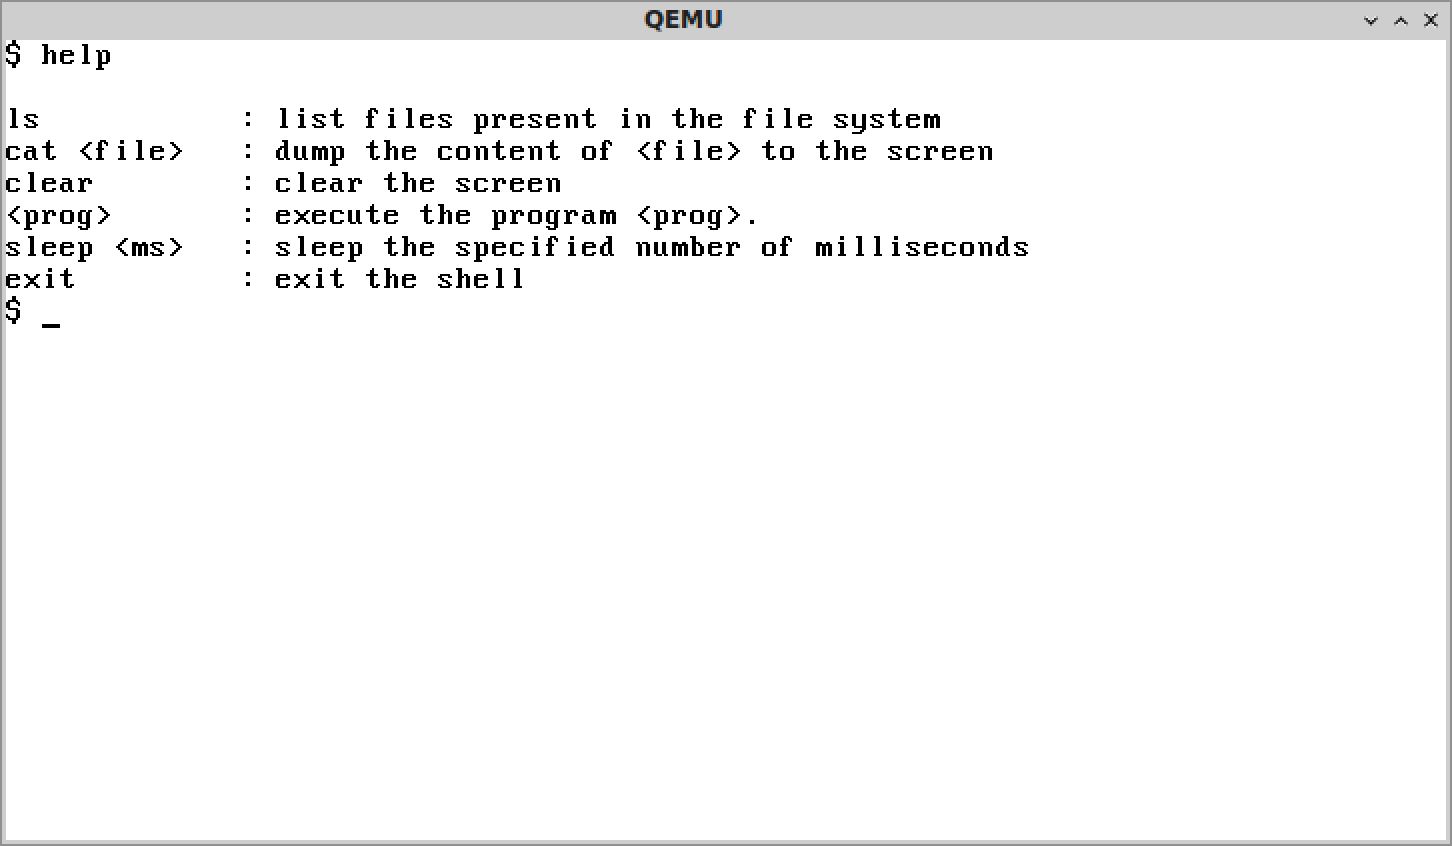
\includegraphics[scale=.6]{images/shell.png}
  \caption{Shell développé}
  \label{mem_view_user}
\end{figure}

\paragraph{Démo} \mbox{} \\
En plus du shell, une démo a été développée afin de valider toutes les fonctionnalités
de l'\acrshort{os}. Cette démo appelle toute les fonctions de la librairie système
et teste l'allocation mémoire dynamique.

%%%%%%%%%%%%%%%%%%%%%%%%%%%%%%%%%%%%%%%%%%%%%%%%%%%%%%%%%%%%%%%%%%
%%%%%%%%%%%%%%%%%%%%%%%%%%%%%%%%%%%%%%%%%%%%%%%%%%%%%%%%%%%%%%%%%%

\newpage
\section{Discussions}
\subsection{Comparaison entre C et Rust}
\subsubsection{Avantages du langage Rust}
\paragraph{Sécurité} :
un avantage principal du langage Rust par rapport au langage C est son compilateur.
Beaucoup d'erreurs dans les programmes en C viennent du programmeur et du laxisme
du compilateur C. Toutes les erreurs liées à la manipulation de la mémoire sont
traitées directement à la compilation d'un programme Rust. Les variable immutables
par défaut ainsi que le concept d'\textit{ownership} oblige le programmeur à faire
un programme sécurisé au niveau de la manipulation de la mémoire.

\paragraph{Langage moderne} :
Rust étant un langage moderne, il emprunte de nombreux concepts à d'autres langages.
Les structures et les traits permettent de faire de la programmation orientée objet.
Par exemple dans notre \acrshort{os}, l'implémentation de la macro \mintinline{rust}{print!}
permettant d'afficher une chaîne de caractères formatée a été extrêment simple et
rapide. Ceci a été permis grâce au concept de trait et à la manipulation de chaînes
de caractères native à Rust.

\paragraph{Flexibilité} :
Rust est aussi beaucoup plus flexible que C. Des librairies peuvent être ajoutées
au projet directement avec Cargo et \href{https://crates.io}{Crates.io}. De plus,
Cargo permet aisément de faire des tests unitaires, de générer de la documentation
pour le code et d'exécuter un projet avec de nombreuses dépendances.

\paragraph{Rapidité} :
un dernier avantage de Rust sont ses performances. D'après le site
\href{https://benchmarksgame-team.pages.debian.net/benchmarksgame/}{Benchmarks Game},
Rust est presque aussi performant que le C \cite{ref30}. Le langage Rust arrive
donc a avoir presque les mêmes performances que le C tout en étant plus sécurisé,
plus moderne et plus flexible.

\subsubsection{Inconvénients du langage Rust}
\paragraph{Documentation} :
actuellement, un des gros inconvénients de Rust est sa documentation. Le langage
étant récent, il est difficile de trouver des exemples sur internet. Il est vrai
que l'équipe de Rust fournit des documents (livre de Rust, de Cargo, exemples, etc)
mais ceux-ci restent légèrement incomplets au sujet des fonctionnalités avancées
de Rust.

\paragraph{Taille des exécutables} :
le langage Rust offre de nombreux mécanismes de sécurité. Il est moderne et possède
beaucoup de fonctionnalités. Le problème ici est que toutes ces fonctionnalités
et mécanismes viennent augmenter la taille de l'exécutable généré par le compilateur.
Un simple programme affichant une chaîne de caractères sur la sortie standard peut
faire jusqu'à 500'000 octets alors qu'en C le même programme aurait une taille de
8000 octets. Dans le chapitre \ref{sec:user:compil}, des méthodes ont été
données pour diminuer la taille d'un exécutable. Cependant, ces méthodes suppriment
certains mécanismes de Rust. Ces problèmes font qu'il est difficile d'utiliser
Rust dans des systèmes embarqués là où C est indispensable.

%%%%%%%%%%%%%%%%%%%%%%%%%%%%%%%%%%%%%%%%%%%%%%%%%%%%%%%%%%%%%%%%%%

\newpage
\subsection{Problèmes rencontrés}
\subsubsection{Compilation de Rust}
Les plus grandes difficultés du projet ont été rencontrées pour la compilation
du Rust. Le langage et le compilateur sont bien documentés tant qu'on reste
dans de la programmation haut niveau. Il n'y a pas contre que très peu d'informations
sur les options avancées du compilateur. Un premier exemple est le contenu d'un
fichier \textit{target triple}. Toutes les options de ce fichier sont énumérées
dans la documentation de Rust mais il n'y a qu'une simple description, aucun exemple.
De plus, les systèmes d'exploitation en Rust existants sont en général pour une
architecture 64 bits. Il a donc aussi été compliqué de trouver des exemples pour
l'architecture utilisée (\acrshort{IA-32}). Un autre exemple est la compilation
d'un programme Rust en format binaire (expliquée dans la partie \ref{sec:user:compil}).
Pour rappel, afin de compiler le code Rust en fichier objet destiné à un format
binaire, il faut utiliser l'option \mintinline{text}{-C relocation_model=static}.
D'après la documentation de la structure \mintinline{text}{Target}, l'option
\mintinline{text}{relocation_model} peut être mise directement dans le
\textit{target triple} sans passer par les options du compilateur \cite{ref29}.
En réalité, l'option ne marche pas lorsqu'elle est mise dans le fichier \textit{target},
il est impératif de spécifier l'option à Xargo.

\subsubsection{Librairie \mintinline{text}{core}}
La librairie \mintinline{text}{core}, bien que très pratique pour la réalisation
de ce travail, a été la source de quelques problèmes. Cette librairie constitue
la base de Rust. Sans cette librairie il ne serait même pas possible de faire une
addition avec l'opérateur '\mintinline{text}{+}'. L'ennui est qu'elle offre aussi
de nombreux mécansimes de protection tel que la macro \mintinline{text}{panic!}.
Tous ces mécanismes réprésentent une place considérable dans un programme Rust
compilé statiquement. Une solution a finalement été trouvé et détaillée dans le
chapitre \ref{sec:user:compil} mais avant de comprendre que les programmes utilisateurs
ne marchaient pas pour cette raison, il a fallu énormément investiguer.

\subsubsection{Passage à la pagination}
Le passage de la gestion mémoire par segmentation à la pagination a été l'origine
de quelques difficultés. Peu de documentation est disponible à ce sujet sur internet.
Des exemple peuvent être trouvés mais aucun n'a fonctionné dans le cas de notre
\acrshort{os}. Le plus compliqué a été de déplacer le \textit{kernel} à la fin
de la \acrshort{ram}. Ensuite il a fallu refaire la gestion des applications
utilisateurs en utilisant la pagination. Il n'y a aucune information implicite
sur l'utilisation du champ \mintinline{text}{cr3} du \acrshort{tss} dans la documentation
d'Intel. Tout a été trouvé de manière empirique en regardant le comportement
du \textit{kernel} lorsque des paramètres sont changés. De plus, quand il y a
un problème au niveau de la pagination, le processeur lève en général l'exception
\textit{Triple Fault} qui a pour conséquence de faire redémarrer QEMU. Il est
donc plus compliqué de corriger les erreurs car il n'y a plus l'information de
la ligne de code qui a provoqué l'exception.

%%%%%%%%%%%%%%%%%%%%%%%%%%%%%%%%%%%%%%%%%%%%%%%%%%%%%%%%%%%%%%%%%%

\newpage
\subsection{Améliorations possibles}
Actuellement, toutes les fonctionnalités décrites dans ce document marchent
parfaitement. Il n'a malheureusement pas été possible (faute de temps), de démontrer
ces fonctionnalités avec une application utilisateur plus poussée. Une démo a
été développée utilisant l'intégralité des appels systèmes du \textit{kernel}
mais elle ne fait qu'afficher du texte à l'écran. Par exemple, il pourrait être
intéressant de développer un jeu. Ce jeu pourrait avoir un affichage en mode texte
avec l'implémentation d'une librairie comme \mintinline{text}{curses} en C ou bien
un affichage pixel par pixel en changeant le mode de l'écran \acrshort{vga}. \\

Plusieurs améliorations sont aussi possibles au niveau de l'implémentation des
tâches utilisateurs. Une première amélioration pourrait être de gérer les
librairies dans le système. Dans le cas de notre \acrshort{os}, on pourrait
ainsi avoir la librairie système stockée dans le système de fichiers et les
applications utilisateurs feraient appel à cette dernière plutôt que d'être
chacun compilé statiquement. Cela implique d'avoir des pages partagées entre plusieurs
tâches. Une autre amélioration possible pourrait être la gestion de la concurrence
afin d'exécuter plusieurs tâches en parallèle. A l'heure actuelle, quand plusieurs
tâches sont exécutées en même temps, elles sont impriquées. Une tâche en appelle
une autre et elle reprend son exécution quand la nouvelle tâche a fini la sienne. \\

Il pourrait aussi être intéressant d'améliorer le système de fichiers. Pour le
moment le système de fichiers est très basique. Tous les fichiers sont ajoutés
à la racine, il n'est pas possible d'écrire, il y a une limite de stockage
de fichiers très basse. Toutes ces fonctionnalités actuellement non disponibles
pourraient être rajoutées. On pourrait même imaginer un autre système de fichiers
que \acrshort{fat} qui serait plus moderne.

%%%%%%%%%%%%%%%%%%%%%%%%%%%%%%%%%%%%%%%%%%%%%%%%%%%%%%%%%%%%%%%%%%
%%%%%%%%%%%%%%%%%%%%%%%%%%%%%%%%%%%%%%%%%%%%%%%%%%%%%%%%%%%%%%%%%%

\newpage
\section{Conclusion}
Ce projet avait plusieurs objectifs. Il fallait dans un premier temps prendre
en main le langage de programmation Rust afin de développer un système d'exploitation
\textit{bare metal}. Ce projet reposait beaucoup sur le cours de programmation
système avancée de l'orientation logiciels et systèmes complexes à hepia. Etant
en orientation matérielle, il a fallu étudier ce sujet en plus du langage Rust.
Ce projet a donc été pour une grande partie un travail de recherche sur le Rust
et sur la conception d'un système d'exploitation pour processeurs Intel 32 bits. \\

Un système d'exploitation simple a finalement été développé. Il est intégralement
en Rust (à l'exception de certaines fonctions en assembleur). Beaucoup
de code a du être mis en \mintinline{text}{unsafe}. Il n'a pas été possible de faire
autrement car nous sommes obligés de faire des manipulations mémoires considérées
\mintinline{text}{unsafe} par le compilateur de Rust. Le mot-clé \mintinline{text}{unsafe}
a tout de même été utilisé avec parcimonie car un des plus gros avantages de Rust
est son compilateur. Mettre l'intégralité du code \mintinline{text}{unsafe} reviendrait
à coder en C. Les objectifs internes à l'implémentation du système d'exploitation
ont aussi été atteints. La gestion de la mémoire par pagination est fonctionnelle. 
Il est aussi possible d'allouer de la mémoire dynamiquement en tant qu'utilisateur
avec les fonctions \mintinline{rust}{malloc} et \mintinline{rust}{free} de la
librairie système implémentée. Des périphériques sont utilisés (affichage \acrshort{vga},
\textit{timer} et clavier). Ils sont gérés grâce aux ports d'entrées/sorties
et aux interruptions. Un mécanisme de commutation de tâches a été implémenté
permettant d'exécuter des applications utilisateurs. Par ailleurs, un shell
a été développé rendant l'\acrshort{os} plus intéractif. \\

Ce projet a aussi permis d'examiner le langage Rust. Il est vrai que c'est un
langage très performant et sécurisé. Il a beaucoup d'avantages par rapport
au C et ses inconvénients sont présents surtout car il est encore jeune. Il est
fort possible que ce langage remplace un jour le C pour la programmation système
et même pour la conception d'\acrshort{os}. Le système d'exploitation Redox est
d'ailleurs entièrement fait en Rust \cite{ref31}. Il est tout de même difficile
de voir un jour Rust remplacer complètement le C. En effet, il semble encore trop
haut niveau pour les systèmes embarqués. \\

En conclusion, je dirais que ce projet a été très instructif. N'ayant pas fait le
cours de programmation système avancée, j'étais très motivé à l'idée de réaliser
ce travail. La programmation système est un domaine qui m'intéresse beaucoup
car il fait le lien entre le matériel et le logiciel. De plus, j'ai eu l'occasion
d'apprendre un nouveau langage : le Rust. Je pense que ce langage a de l'avenir
et que connaitre ses spécificités pourra être bénéfique pour plus tard. Je serais
aussi curieux de voir ce qu'il pourrait donner dans la programmation pour systèmes
embarqués.


%%%%%%%%%%%%%%%%%%%%%%%%%%%%%%%%%%%%%%%%%%%%%%%%%%%%%%%%%%%%%%%%%%
%%%%%%%%%%%%%%%%%%%%%%%%%%%%%%%%%%%%%%%%%%%%%%%%%%%%%%%%%%%%%%%%%%

\newpage
\section*{Références}
\addcontentsline{toc}{section}{Références}
\nocite{*}
\bibliographystyle{unsrt}
\bibliography{biblio}

%%%%%%%%%%%%%%%%%%%%%%%%%%%%%%%%%%%%%%%%%%%%%%%%%%%%%%%%%%%%%%%%%%
%%%%%%%%%%%%%%%%%%%%%%%%%%%%%%%%%%%%%%%%%%%%%%%%%%%%%%%%%%%%%%%%%%

\newpage
\section*{Annexe A : Code source}
\addcontentsline{toc}{section}{Annexe A : Code source}
Le code source du projet est disponible en annexe au format papier ou au format
électronique à l'adresse \url{https://github.com/orpheeantoniadis/RustOS}.

\newpage
\section*{Annexe B : Installation}
\addcontentsline{toc}{section}{Annexe B : Installation}
Ci dessous, les étapes d'installation du système d'exploitation. Toutes les
commandes sont à exécuter dans un shell d'une distribution Linux. \\

\paragraph{Configuration de Linux} \mbox{} \\
\begin{minted}[tabsize=4,frame=single,bgcolor=bg]{shell}
sudo apt-get install git curl nasm qemu
\end{minted}

\paragraph{Configuration de Rust} \mbox{} \\
\begin{minted}[tabsize=4,frame=single,bgcolor=bg]{shell}
curl https://sh.rustup.rs -sSf | sh
echo source $HOME/.cargo/env >> ~/.bashrc
rustup override add nightly
cargo install xargo
rustup component add rust-src
\end{minted}

\paragraph{Compilation} \mbox{} \\
\begin{minted}[tabsize=4,frame=single,bgcolor=bg]{shell}
git clone git@github.com:orpheeantoniadis/RustOS.git
cd RustOS
make build
\end{minted}

\paragraph{Exécution} \mbox{} \\
\begin{minted}[tabsize=4,frame=single,bgcolor=bg]{shell}
make run
\end{minted}

\paragraph{Documentation} \mbox{} \\
\begin{minted}[tabsize=4,frame=single,bgcolor=bg]{shell}
make doc
\end{minted}

\end{document}
